\documentclass{article}
\usepackage[utf8]{inputenc}
\usepackage{graphicx}
\begin{document}

% Титульный лист (ГОСТ Р 7.0.11-2001, 5.1)
\thispagestyle{empty}
\begin{center}
\thesisOrganization
\end{center}
%
\vspace{0pt plus4fill} %число перед fill = кратность относительно некоторого расстояния fill, кусками которого заполнены пустые места
\IfFileExists{images/logo.png}{
  \begin{minipage}[b]{0.5\linewidth}
    \begin{flushleft}
      \includegraphics[height=3.5cm]{logo}
    \end{flushleft}
  \end{minipage}%
  \begin{minipage}[b]{0.5\linewidth}
    \begin{flushright}
      На правах рукописи\\
%      \textsl {УДК \thesisUdk}
    \end{flushright}
  \end{minipage}
}{
\begin{flushright}
На правах рукописи

%\textsl {УДК \thesisUdk}
\end{flushright}
}
%
\vspace{0pt plus6fill} %число перед fill = кратность относительно некоторого расстояния fill, кусками которого заполнены пустые места
\begin{center}
{\large \thesisAuthor}
\end{center}
%
\vspace{0pt plus1fill} %число перед fill = кратность относительно некоторого расстояния fill, кусками которого заполнены пустые места
\begin{center}
\textbf {\large %\MakeUppercase
\thesisTitle}

\vspace{0pt plus2fill} %число перед fill = кратность относительно некоторого расстояния fill, кусками которого заполнены пустые места
{%\small
Специальность \thesisSpecialtyNumber\ "---

<<\thesisSpecialtyTitle>>
}

\ifdefined\thesisSpecialtyTwoNumber
{%\small
Специальность \thesisSpecialtyTwoNumber\ "---

<<\thesisSpecialtyTwoTitle>>
}
\fi

\vspace{0pt plus2fill} %число перед fill = кратность относительно некоторого расстояния fill, кусками которого заполнены пустые места
Диссертация на соискание учёной степени

\thesisDegree
\end{center}
%
\vspace{0pt plus4fill} %число перед fill = кратность относительно некоторого расстояния fill, кусками которого заполнены пустые места
\begin{flushright}
\ifdefined\supervisorTwoFio
Научные руководители:

\supervisorRegalia

\ifdefined\supervisorDead
\framebox{\supervisorFio}
\else
\supervisorFio
\fi

\supervisorTwoRegalia

\ifdefined\supervisorTwoDead
\framebox{\supervisorTwoFio}
\else
\supervisorTwoFio
\fi
\else
Научный руководитель:

\supervisorRegalia

\ifdefined\supervisorDead
\framebox{\supervisorFio}
\else
\supervisorFio
\fi
\fi

\end{flushright}
%
\vspace{0pt plus4fill} %число перед fill = кратность относительно некоторого расстояния fill, кусками которого заполнены пустые места
{\centering\thesisCity\ "--- \thesisYear\par}


% !TEX encoding = UTF-8
% !TEX program = lualatex

\chapter*{Введение}                         % Заголовок
\addcontentsline{toc}{chapter}{Введение}    % Добавляем его в оглавление

\newcommand{\actuality}{{\textbf\actualityTXT}}
\newcommand{\progress}{{\textbf\progressTXT}}
\newcommand{\aim}{{\textbf\aimTXT}}
\newcommand{\tasks}{\textbf{\tasksTXT}}
\newcommand{\novelty}{\textbf{\noveltyTXT}}
\newcommand{\influence}{\textbf{\influenceTXT}}
\newcommand{\methods}{\textbf{\methodsTXT}}
\newcommand{\defpositions}{\textbf{\defpositionsTXT}}
\newcommand{\reliability}{\textbf{\reliabilityTXT}}
\newcommand{\probation}{\textbf{\probationTXT}}
\newcommand{\contribution}{\textbf{\contributionTXT}}
\newcommand{\publications}{\textbf{\publicationsTXT}}

\begin{comment}
{\actuality}
Современный ландшафт киберугроз характеризуется ростом сложности, целенаправленности и скрытности атак. Особенно опасны многоэтапные целевые атаки, осуществляемые как государственными акторами (например, TAO, Unit 8200), так и финансово мотивированными группировками (FIN7, Carbanak). Такие атаки часто остаются незамеченными длительное время, поскольку традиционные системы обнаружения вторжений (IDS), основанные на~сигнатурном анализе, эффективны лишь против известных угроз и не способны выявлять новые или модифицированные тактики. Методы аномального анализа, в~свою очередь, страдают от высокого уровня ложных срабатываний и~низкой интерпретируемости.

В этих условиях возрастает потребность в~семантически богатых моделях, способных отражать не отдельные события, а логические цепочки компрометации, включающие тактики, техники и~процедуры (TTPs), описанные в фреймворке MITRE ATT\&CK. Классические графы и~даже гиперграфы не всегда адекватно передают сложные взаимодействия между множествами сущностей в ИТ-инфраструктуре.

Метаграфы — обобщение гиперграфов — позволяют моделировать зависимости, в~которых как источники, так и цели действия могут быть множествами объектов. Расширение метаграфов за счёт атрибутивного слоя (привязка временных, контекстных и семантических характеристик к вершинам и дугам) открывает возможности для точного моделирования поведения атакующих и последующего сопоставления с данными телеметрии.

Актуальность темы обусловлена необходимостью повышения эффективности систем обнаружения целевых многоэтапных атак за счёт разработки новой формальной модели на основе атрибутивных метаграфов. Предложенная методика обеспечивает интерпретируемость результатов, адаптацию к эволюции тактик злоумышленников и снижение числа ложных срабатываний, что особенно важно для защиты критически важных инфраструктур.

{\progress}
Проблема моделирования и обнаружения компьютерных атак активно исследуется с конца 1990-х годов. Ранние работы О.~Шейнера заложили основы графов атак. В 2000-х годах получили развитие деревья атак. С появлением фреймворка MITRE ATT\&CK (2013) возникла потребность в онтологических моделях.

Параллельно развивались подходы на основе машинного обучения, включая графовые нейросети (GNN). Однако такие системы часто являются «чёрными ящиками». Применение метаграфов в кибербезопасности остаётся малоизученным. Отдельные работы (например, \cite{Latypov2020}) намечают потенциал метаграфов, но не предлагают полной методики выявления или экспериментальной валидации на данных реальных APT.

Таким образом, в научной литературе отсутствует целостная методика, объединяющая формальную модель атрибутивного метаграфа, алгоритмы построения и сопоставления, интеграцию с MITRE ATT\&CK и экспериментальную оценку на данных реальных атак.

{\aim} диссертационного исследования является разработка и экспериментальная валидация модели, метода и методики выявления компьютерных атак на основе атрибутивных метаграфов, обеспечивающей высокую точность обнаружения многоэтапных угроз при приемлемых вычислительных затратах.

Для~достижения поставленной цели необходимо было решить следующие {\tasks}:
\begin{enumerate}[beginpenalty=10000]
    \item Провести анализ существующих методов моделирования и выявления компьютерных атак, выявить их недостатки и ограничения.
    \item Формализовать понятие атрибутивного метаграфа в контексте кибербезопасности.
    \item Разработать методику построения динамических атрибутивных метаграфов на основе данных телеметрии.
    \item Создать алгоритм сопоставления шаблонов атак с текущим состоянием защищаемой системы.
    \item Провести имитационное моделирование на данных реальных APT-кампаний.
    \item Реализовать прототип программной системы и оценить её эффективность.
\end{enumerate}

{\novelty}
\begin{enumerate}[beginpenalty=10000]
    \item Впервые предложена модель атрибутивного метаграфа для представления цепочек компрометации, интегрированная с таксономией MITRE ATT\&CK.
    \item Разработан алгоритм частичного изоморфизма атрибутивных метаграфов, учитывающий семантическое сходство атрибутов и временные окна.
    \item Предложена метрика риска компрометации, основанная на взвешенной сумме вероятностей реализации критических путей в метаграфе.
    \item Введено понятие динамического метаграфа безопасности, обновляемого инкрементально.
\end{enumerate}

\textbf{Теоретическая значимость} состоит в расширении аппарата формальных моделей кибербезопасности за счёт введения атрибутивных метаграфов.

{\influence} подтверждена реализацией прототипа системы обнаружения, который интегрируется с существующими SIEM/SOAR-платформами через API, поддерживает импорт шаблонов атак в формате STIX~2.1 и снижает нагрузку на SOC за счёт повышения точности алертов. Результаты внедрены в пилотном проекте SOC-центра.

{\methods} В работе использован комплексный методологический подход, включающий теоретический анализ, формальное моделирование, алгоритмический синтез, имитационное моделирование и экспериментальную оценку.

\textbf{Объектом} исследования являются процессы выявления компьютерных атак.  
\textbf{Предметом} — методы и модели на основе атрибутивных метаграфов.

{\defpositions}
\begin{enumerate}[beginpenalty=10000]
    \item Атрибутивные метаграфы обеспечивают адекватную формальную модель для представления многоэтапных компьютерных атак.
    \item Разработанный алгоритм сопоставления эталонных и динамических метаграфов позволяет эффективно выявлять атаки с высокой точностью и низким уровнем ложных срабатываний.
    \item Прототип системы, реализующий предложенную методику, демонстрирует практическую применимость подхода в реальных условиях эксплуатации.
\end{enumerate}

{\reliability} полученных результатов обеспечивается корректным применением математического аппарата, воспроизводимостью экспериментов и согласованностью с известными фактами о тактиках злоумышленников.

{\probation}
Результаты диссертационной работы докладывались на:
\begin{itemize}
    \item Российская научно-техническая конференция (Москва, 2021);
    \item XXI Всероссийская научно-практическая конференция (Киров, 2021);
    \item CyberSecurityDays (Санкт-Петербург, 2025).
\end{itemize}

{\contribution}
Все результаты получены автором самостоятельно. Под руководством научного руководителя автор участвовал в постановке задачи, разработке модели, создании методики и экспериментальной оценке на данных APT.

{\publications}
Основные результаты по теме диссертации изложены в~7~печатных изданиях,  
3 из которых опубликованы в журналах, рекомендованных ВАК и индексируемых Scopus,  
2 — в виде патентов,  
2 — в виде свидетельств о регистрации программ для ЭВМ.

\end{comment}
%\begin{comment}

{\actuality}
Современный ландшафт киберугроз характеризуется ростом сложности, целенаправленности и скрытности атак. Особенно опасны многоэтапные целевые атаки, осуществляемые как государственными акторами (например, TAO, Unit 8200), так и финансово мотивированными группировками FIN7, Carbanak, Lazarus. Такие атаки часто остаются незамеченными длительное время, поскольку тактики злоумышленников и~гарантировать интерпретируемость результатов для аналитиков центров мониторинга безопасности (SOC)
\ifsynopsis
\else
    \nomenclature{SOC}{Security Operations Center, центр мониторинга безопасности}
\fi.

Традиционные системы обнаружения вторжений (IDS)
\ifsynopsis
\else
    \nomenclature{IDS/IPS}{Intrusion Detection Systems / Intrusion Prevention Systems, системы обнаружения и предотвращения вторжений}
\fi, основанные на~сигнатурном анализе, эффективны лишь против известных угроз и~не~способны выявлять новые или модифицированные тактики. Методы аномального анализа, в свою очередь, страдают от высокого уровня ложных срабатываний и~низкой интерпретируемости, что приводит к информационной перегрузке аналитиков и~снижению оперативности реагирования.

В этих условиях возрастает потребность в семантически богатых моделях, способных отражать не отдельные события, а логические цепочки компрометации, включающие тактики, техники и процедуры (TTPs)
\ifsynopsis
\else
    \nomenclature{TTPs}{Tactics, Techniques, and Procedures, тактики, техники и процедуры}
\fi, описанные в фреймворке MITRE ATT\&CK. Классические графы и даже гиперграфы не~всегда адекватно передают сложные взаимодействия между множествами сущностей в ИТ-инфраструктуре.

Метаграфы — обобщение гиперграфов — позволяют моделировать зависимости, в которых как источники, так и цели действия могут быть множествами объектов. Расширение метаграфов за счёт атрибутивного слоя (привязка временных, контекстных и семантических характеристик к вершинам и дугам) открывает возможности для точного моделирования поведения атакующих и последующего сопоставления с данными телеметрии.

\ifsynopsis
Актуальность темы обусловлена необходимостью повышения\linebreak эффективность систем обнаружения целевых многоэтапных атак за счёт разработки новой формальной модели на основе атрибутивных метаграфов. Предложенная методика обеспечивает интерпретируемость результатов, адаптацию к эволюции тактик злоумышленников и~снижение числа ложных срабатываний, что особенно важно для защиты критически важных инфраструктур, включая железнодорожный транспорт.
\else

Проблема моделирования и обнаружения компьютерных атак активно исследуется с конца 1990-х годов. Ранние работы О.~Шейнера \autocite{Schneier1999} заложили основы графов атак, где уязвимости и условия компрометации представлены в виде логических зависимостей. Однако такие модели статичны и не учитывают динамику реальных атак.

В 2000-х годах получили развитие деревья атак \autocite{Sheyner2002}, позволяющие иерархически декомпозировать цель атаки. Несмотря на наглядность, они плохо масштабируются на сложные сценарии с параллельными и циклическими действиями.

С появлением фреймворка MITRE ATT\&CK (2013) возникла потребность в онтологических моделях, способных интегрировать знания о TTPs. Работы, такие как CALDERA \autocite{CALDERA2017} и Atomic Red Team \autocite{AtomicRedTeam}, продемонстрировали возможность автоматизированного моделирования атак, но не решили проблему обнаружения в реальных средах.

Параллельно развивались подходы на основе машинного обучения: от простых классификаторов до глубоких нейронных сетей и графовых нейросетей (Graph Neural Networks, GNN)
\ifsynopsis
\else
    \nomenclature{GNN}{Graph Neural Networks, графовые нейросети}
\fi. Однако такие системы часто являются «чёрными ящиками», что затрудняет верификацию и доверие со стороны аналитиков.

Применение метаграфов в кибербезопасности остаётся малоизученным. Отдельные работы (например, \cite{Latypov2020}) намечают потенциал метаграфов для моделирования угроз, но не предлагают полной методики выявления, алгоритмов сопоставления или экспериментальной валидации на данных реальных APT.

Таким образом, в научной литературе отсутствует целостная методика, объединяющая формальную модель атрибутивного метаграфа, алгоритмы построения и сопоставления, интеграцию с MITRE ATT\&CK и экспериментальную оценку на данных реальных атак.

Важнейшей областью применения подобной методики является защита критически важных инфраструктур, в том числе железнодорожного транспорта. Безопасность информационной инфраструктуры (ИИ)
\ifsynopsis
\else
    \nomenclature{ИИ}{информационная инфраструктура}
\fi железнодорожного транспорта (ЖТ)
\ifsynopsis
\else
    \nomenclature{ЖТ}{железнодорожный транспорт}
\fi в условиях роста интенсивности и результативности компьютерных атак определяется эффективностью и адекватностью реализуемых мер защиты на всех уровнях ИИ.

Учитывая исключительную важность деятельности ЖТ для Российской Федерации, вопросы обеспечения информационной безопасности (ИБ)
\ifsynopsis
\else
\nomenclature{ИБ}{информационная безопасность}
\fi должны занимать первостепенное место при формировании и развитии ИИ ЖТ. Деятельность по обеспечению ИБ автоматизированной системы управления пассажирскими перевозками (АСУ ПП)
\ifsynopsis
\else
\nomenclature{АСУ ПП}{автоматизированная система управления пассажирскими перевозками}
\fi должна быть направлена на поддержание основных бизнес-процессов и устойчивое функционирование компании в условиях реализации компьютерных атак.

Современные требования регуляторов (Федеральный закон № 187-ФЗ, постановление Правительства РФ № 127, ГОСТ Р ИСО/МЭК 27002–2021, приказы ФСТЭК России № 235, № 239) предполагают переход от оценки воздействий на свойства информации (конфиденциальность, целостность, доступность) к оценке влияния инцидентов на бизнес-процессы. Реализация этого подхода требует разработки методического аппарата, способного связывать технические артефакты атак с последствиями для операционной деятельности, что и обеспечивает предлагаемая методика на основе атрибутивных метаграфов.
\fi

% Этот раздел должен быть отдельным структурным элементом по
% ГОСТ, но он, как правило, включается в описание актуальности
% темы. Нужен он отдельным структурынм элемементом или нет ---
% смотрите другие диссертации вашего совета, скорее всего не нужен.

{\progress}

Разработка и создание эффективных систем обеспечения информационной безопасности автоматизированных, информационных и телекоммуникационных систем (АИТС)
\ifsynopsis
\else
\nomenclature{АИТС}{автоматизированные, информационные и телекоммуникационные системы}
\fi 
критического применения остаётся одной из ключевых научно-технических задач современности. В её решении значительный вклад внесли отечественные исследователи, развившие как теоретические основы, так и прикладные методы защиты критически важных инфраструктур.

Особое место в этом направлении занимают работы Зегжды Д. П., Зегжды П.Д. и~их научной школы, заложившие основы системного подхода к управлению безопасностью в~условиях динамически меняющихся угроз. В частности, им предложена многоуровневая архитектура автоматизированного управления безопасностью компьютерных систем \autocite{Zegzhda2020}, а также методы оценки устойчивости киберфизических систем к целенаправленным деструктивным воздействиям \autocite{Pavlenko2018}. Совместно с М. О. Калининым разработаны модели программно-определяемого управления безопасностью для крупномасштабных сетей \autocite{Kalinin2018}, что особенно актуально для распределённых АИТС железнодорожного транспорта.

Значительный вклад в развитие методов формализации и управления информационной безопасностью на основе онтологических моделей внесли работы А.~А.~Корниенко и соавторов (Д.~Н.~Бирюков, М.~Л.~Глухарев, А.~П.~Глухов, С.~В.~Диасамидзе). В~исследовании 2017~года предложена модель онтологического представления процессов и метод синтеза спецификаций для интеллектуальной системы риск-ориентированного упреждающего управления ИБ, опубликованная в журнале «Известия Петербургского университета путей сообщения»~\autocite{Kornienko2017}. Данный подход позволил сместить фокус с реактивного мониторинга на проактивное управление рисками за счёт формализации взаимосвязей между бизнес-процессами, угрозами и мерами защиты. Вместе с тем, предложенная модель носит преимущественно статический характер, не учитывает динамическую эволюцию многоэтапных атак в~реальном времени и~не опирается на современные таксономии TTPs, такие как MITRE ATT\&CK. Это определяет необходимость развития онтологического подхода в~сторону динамических графовых структур, способных отражать причинно-следственные цепочки компрометации с~учётом семантических атрибутов, временных окон и~критичности информационных активов.

 Котенко И. В. и Саенко И. Б. внесли существенный вклад в архитектурное проектирование интеллектуальных сервисов защиты информации в критической инфраструктуре \autocite{Kotenko2013}, предложив подходы к построению распределённых систем обнаружения вторжений на основе мультиагентных технологий. Эти идеи получили дальнейшее развитие в работах по оценке управляемости мультиагентных систем с использованием многоуровневых графовых моделей \autocite{Zegzhda2016}.

Отдельного внимания заслуживает вклад Петренко А. А. в формализацию контроля целостности в~доверенной информационной среде \autocite{Zegzhda2020}, что остаётся актуальным при построении защищённых архитектур для АСУ ТП.

На основе указанных исследований определены принципы управления рисками и разработаны методы выявления уязвимостей, обнаружения атак и ликвидации их последствий в критически важных инфраструктурах, включая железнодорожный транспорт.

Вместе с тем, проблема оценки влияния компьютерных инцидентов на бизнес-процессы организаций, особенно в секторе транспорта, остаётся недостаточно исследованной и требует дальнейшей разработки — в том числе за счёт интеграции методов моделирования атак (например, на основе атрибутивных метаграфов) с моделями бизнес-непрерывности и оценки операционного риска.

{\aim} диссертационного исследования повышение — эффективности систем обнаружения целевых многоэтапных атак в центрах мониторинга безопасности (SOC) за счёт разработки и внедрения методики выявления угроз на основе атрибутивных метаграфов, обеспечивающей высокую точность обнаружения при приемлемых вычислительных затратах и совместимость с существующей SIEM/SOAR-инфраструктурой.


Для~достижения поставленной цели необходимо было решить следующие {\tasks}:

\begin{enumerate}[beginpenalty=10000] % https://tex.stackexchange.com/a/476052/104425  
    \item Провести анализ существующих методов моделирования и выявления компьютерных атак, выявить их недостатки и ограничения.
    \item Разработать формальную модель атрибутивного метаграфа для представления цепочек компрометации, интегрированную с таксономией MITRE ATT\&CK и поддерживающую динамическое обновление на основе событий телеметрии.
    \item На основе предложенной модели разработать методику построения динамических атрибутивных метаграфов и сопоставления их с эталонными паттернами атак, учитывающую семантическое сходство атрибутов, временные окна и критичность информационных активов.
    \item Реализовать прототип программной системы обнаружения атак на основе разработанной методики и оценить её эффективность по стандартным метрикам (точность, полнота, уровень ложных срабатываний, время обработки) в условиях, приближенных к реальным.
    \item Провести имитационное моделирование выявления атак\linebreak c~использованием данных реальных кампаний APT и финансово мотивированных группировок.
    \item Обеспечить совместимость разработанного решения с существующей инфраструктурой безопасности (SIEM/SOAR), отечественными стандартами (ФСТЭК, ГОСТ Р 56939–2024) и международными фреймворками (MITRE ATT\&CK, STIX 2.1).
\end{enumerate}

Для экспериментальной оценки разработанной методики была создана изолированная тестовая платформа на базе CALDERA~4.0 и Proxmox~VE~8.1, включающая:
\begin{itemize}
    \item \textbf{Источники телеметрии}: EDR-агенты (Sysmon), аудит-логи ОС (Auditd), сетевые логи Zeek (conn.log, http.log);
    \item \textbf{Система нормализации}: Logstash с парсерами в формате Elastic Common Schema (ECS);
    \item \textbf{Хранилище событий}: Elasticsearch 8.7;
    \item \textbf{Движок анализа}: Python~3.11 + NetworkX + кастомный VF2-алгоритм для поиска частичного изоморфизма;
    \item \textbf{Визуализация}: Grafana с панелями по kill chain и MITRE ATT\&CK Navigator.
\end{itemize}

Тестовые данные включали:
\begin{itemize}
    \item 50 сценариев атак в CALDERA (Log4Shell, phishing, PowerShell lateral movement, DNS tunneling) по тактикам MITRE ATT\&CK;
    \item 10 млн легитимных событий от корпоративной сети банка (30 дней аудита Windows/Linux);
    \item 12 реальных инцидентов, размеченных ИБ-командой (целевые фишинг-атаки с exfiltration).
\end{itemize}

{\novelty}
\begin{enumerate}[beginpenalty=10000] % https://tex.stackexchange.com/a/476052/104425  
    \item Предложена метрика риска компрометации, основанная на взвешенной сумме вероятностей реализации критических путей в метаграфе и позволяющая учитывать как структуру атаки, так и бизнес-важность целевых информационных активов.
    \item Введено понятие динамического метаграфа безопасности, обновляемого инкрементально по мере поступления новых событий телеметрии, что обеспечивает адаптивность модели к эволюции тактик злоумышленников.
    \item Впервые предложена модель атрибутивного метаграфа для представления цепочек компрометации, интегрированная с таксономией MITRE ATT\&CK и обладающая возможностью семантически насыщенного описания многоэтапных атак за счёт привязки атрибутов к вершинам и гипердугам.
    \item Разработан алгоритм частичного изоморфизма атрибутивных метаграфов, учитывающий семантическое сходство атрибутов и временные окна, что позволяет эффективно выявлять атаки, использующие обфускацию и Living-off-the-Land техники, при сохранении высокой точности сопоставления.
\end{enumerate}

\textbf{Теоретическая значимость} состоит в расширении аппарата формальных моделей кибербезопасности за счёт введения атрибутивных метаграфов, что создаёт основу для дальнейших исследований в области семантического анализа угроз.

{\influence} подтверждена реализацией прототипа системы обнаружения, который интегрируется с существующими\linebreak SIEM/SOAR-платформами через API, поддерживает импорт шаблонов атак в формате STIX~2.1, позволяет аналитикам визуализировать обнаруженные цепочки в виде интерактивных графов и снижает нагрузку на SOC за счёт повышения точности оповещений.

{\methods} В работе использован\linebreak комплексный методологический подход, включающий теоретический анализ, формальное моделирование, алгоритмический синтез, имитационное моделирование, экспериментальную оценку и прототипирование.

\textbf{Объектом} исследования являются процессы выявления компьютерных атак в информационных системах.  

\textbf{Предметом} исследования выступают методы и модели, основанные на атрибутивных метаграфах, применяемые для представления и обнаружения цепочек компрометации.

{\defpositions}
\begin{enumerate}[beginpenalty=10000] % https://tex.stackexchange.com/a/476052/104425  
    \item Формальная модель на основе атрибутивны метааграфов для представления многоэтапных компьютерных атак.
    \item Алгоритм сопоставления эталонных и динамических метаграфов, позволяющий эффективно выявлять атаки с высокой точностью и низким уровнем ложных срабатываний.
    \item Прототип системы, реализующий предложенную методику, \linebreak демонстрирующий практическую применимость подхода в реальных условиях эксплуатации.
\end{enumerate}

В приложении представлено решение совета из Национального исследовательского Нижегородского государственного университета \linebreak им.~Н.~И.~Лобачевского, где обоснованно даются рекомендации\linebreak по~формулировкам защищаемых положений. Результаты исследования внедрены в пилотном проекте в составе SOC-центра ПАО «Транснефть», где за 3~месяца тестирования система выявила 12~инцидентов, пропущенных стандартными правилами корреляции.

{\reliability} основных научных результатов обеспечивается корректным применением математических методов исследования\linebreak и подтверждается близостью результатов расчетов, полученных с использованием разработанных методов и моделей, с фактически полученными результатами мониторинга реальных объектов, а также апробацией на научно-технических конференциях и публикациями в научных изданиях.

{\probation}

Результаты диссертационной работы докладывались и обсуждались на следующих мероприятиях:

\noindent
\begin{itemize}
    \item IV ежегодной Национальной научно-практической конференции "Цифровизация правосудия: проблемы и перспективы" (Москва, 2025);
    \item Российская научно-технической конференции с международным участием  (Москва, 2021);
    \item XXI Всероссийская научно-практическая конференция (Киров, 2021).
\end{itemize}

{\contribution} Все результаты, выносимые на защиту, получены автором самостоятельно. Под руководством научного руководителя автор лично участвовал в~постановке научной проблемы, формулировке цели и~задач исследования, разработке формальной модели атрибутивного метаграфа, создании методики выявления многоэтапных компьютерных атак на основе данных телеметрии, а~также в~проектировании и реализации экспериментальной оценки эффективности предложенного подхода на данных реальных кампаний APT и финансово мотивированных группировок.
\ifsynopsis
{\structure}
\else
\fi
Диссертация состоит из введения, четырёх глав, заключения, списка литературы и приложений.
Общий объём работы — 128~страниц, содержит 27~рисунков, 11~таблиц,
библиографию из 98~наименований, включая 12 источников на иностранных языках.

\ifnumequal{\value{bibliosel}}{0}
{%%% Встроенная реализация с загрузкой файла через движок bibtex8. (При желании, внутри можно использовать обычные ссылки, наподобие `\cite{vakbib1,vakbib2}`).
    {\publications} Основные результаты по теме диссертации изложены
    в~XX~печатных изданиях,
    X из которых изданы в журналах, рекомендованных ВАК,
    X "--- в тезисах докладов.
}%
{%%% Реализация пакетом biblatex через движок biber
    \begin{refsection}[bl-author, bl-registered]
        % Это refsection=1.
        % Процитированные здесь работы:
        %  * подсчитываются, для автоматического составления фразы "Основные результаты ..."
        %  * попадают в авторскую библиографию, при usefootcite==0 и стиле `\insertbiblioauthor` или `\insertbiblioauthorgrouped`
        %  * нумеруются там в зависимости от порядка команд `\printbibliography` в этом разделе.
        %  * при использовании `\insertbiblioauthorgrouped`, порядок команд `\printbibliography` в нём должен быть тем же (см. biblio/biblatex.tex)
        %
        % Невидимый библиографический список для подсчёта количества публикаций:
        \phantom{\printbibliography[heading=nobibheading, section=1, env=countauthorvak,          keyword=biblioauthorvak]%
        \printbibliography[heading=nobibheading, section=1, env=countauthorwos,          keyword=biblioauthorwos]%
        \printbibliography[heading=nobibheading, section=1, env=countauthorscopus,       keyword=biblioauthorscopus]%
        \printbibliography[heading=nobibheading, section=1, env=countauthorconf,         keyword=biblioauthorconf]%
        \printbibliography[heading=nobibheading, section=1, env=countauthorother,        keyword=biblioauthorother]%
        \printbibliography[heading=nobibheading, section=1, env=countregistered,         keyword=biblioregistered]%
        \printbibliography[heading=nobibheading, section=1, env=countauthorpatent,       keyword=biblioauthorpatent]%
        \printbibliography[heading=nobibheading, section=1, env=countauthorprogram,      keyword=biblioauthorprogram]%
        \printbibliography[heading=nobibheading, section=1, env=countauthor,             keyword=biblioauthor]%
        \printbibliography[heading=nobibheading, section=1, env=countauthorvakscopuswos, filter=vakscopuswos]%
        \printbibliography[heading=nobibheading, section=1, env=countauthorscopuswos,    filter=scopuswos]}%
        %
        \nocite{*}%
        %
        {\publications} Основные результаты по теме диссертации изложены в~\arabic{citeauthor}~печатных изданиях,
        \arabic{citeauthorvak} из которых изданы в журналах, рекомендованных ВАК%
        \ifnum \value{citeauthorscopuswos}>0%
            , \arabic{citeauthorscopuswos} "--- в~периодических научных журналах, индексируемых Web of~Science и~Scopus%
        \fi%
        \ifnum \value{citeauthorconf}>0%
            , \arabic{citeauthorconf} "--- в~тезисах докладов.
        \else%
            .
        \fi%
        \ifnum \value{citeregistered}=1%
            \ifnum \value{citeauthorpatent}=1%
                Зарегистрирован \arabic{citeauthorpatent} патент.
            \fi%
            \ifnum \value{citeauthorprogram}=1%
                Зарегистрирована \arabic{citeauthorprogram} программа для ЭВМ.
            \fi%
        \fi%
        \ifnum \value{citeregistered}>1%
            Зарегистрированы\ %
            \ifnum \value{citeauthorpatent}>0%
            \formbytotal{citeauthorpatent}{патент}{}{а}{}%
            \ifnum \value{citeauthorprogram}=0 . \else \ и~\fi%
            \fi%
            \ifnum \value{citeauthorprogram}>0%
            \formbytotal{citeauthorprogram}{программ}{а}{ы}{} для ЭВМ.
            \fi%
        \fi%
        % К публикациям, в которых излагаются основные научные результаты диссертации на соискание учёной
        % степени, в рецензируемых изданиях приравниваются патенты на изобретения, патенты (свидетельства) на
        % полезную модель, патенты на промышленный образец, патенты на селекционные достижения, свидетельства
        % на программу для электронных вычислительных машин, базу данных, топологию интегральных микросхем,
        % зарегистрированные в установленном порядке.(в ред. Постановления Правительства РФ от 21.04.2016 N 335)
    \end{refsection}%
    \begin{refsection}[bl-author, bl-registered]
        % Это refsection=2.
        % Процитированные здесь работы:
        %  * попадают в авторскую библиографию, при usefootcite==0 и стиле `\insertbiblioauthorimportant`.
        %  * ни на что не влияют в противном случае
        %\nocite{vakbib2}%vak
        %\nocite{patbib1}%patent
        %\nocite{progbib1}%program
        %\nocite{bib1}%other
        %\nocite{confbib1}%conf
    \end{refsection}%
        %
        % Всё, что вне этих двух refsection, это refsection=0,
        %  * для диссертации - это нормальные ссылки, попадающие в обычную библиографию
        %  * для автореферата:
        %     * при usefootcite==0, ссылка корректно сработает только для источника из `external.bib`. Для своих работ --- напечатает "[0]" (и даже Warning не вылезет).
        %     * при usefootcite==1, ссылка сработает нормально. В авторской библиографии будут только процитированные в refsection=0 работы.
}
\begin{comment}

 При использовании пакета \verb!biblatex! будут подсчитаны все работы, добавленные
 в файл \verb!biblio/author.bib!. Для правильного подсчёта работ в~различных
 системах цитирования требуется использовать поля:
 \begin{itemize}
        \item \texttt{authorvak} если публикация индексирована ВАК,
        \item \texttt{authorscopus} если публикация индексирована Scopus,
        \item \texttt{authorwos} если публикация индексирована Web of Science,
        \item \texttt{authorconf} для докладов конференций,
        \item \texttt{authorpatent} для патентов,
        \item \texttt{authorprogram} для зарегистрированных программ для ЭВМ,
        \item \texttt{authorother} для других публикаций.
\end{itemize}
Для подсчёта используются счётчики:
\begin{itemize}
        \item \texttt{citeauthorvak} для работ, индексируемых ВАК,
        \item \texttt{citeauthorscopus} для работ, индексируемых Scopus,
        \item \texttt{citeauthorwos} для работ, индексируемых Web of Science,
        \item \texttt{citeauthorvakscopuswos} для работ, индексируемых одной из трёх баз,
        \item \texttt{citeauthorscopuswos} для работ, индексируемых Scopus или Web of~Science,
        \item \texttt{citeauthorconf} для докладов на конференциях,
        \item \texttt{citeauthorother} для остальных работ,
        \item \texttt{citeauthorpatent} для патентов,
        \item \texttt{citeauthorprogram} для зарегистрированных программ для ЭВМ,
        \item \texttt{citeauthor} для суммарного количества работ.
\end{itemize}
% Счётчик \texttt{citeexternal} используется для подсчёта процитированных публикаций;
% \texttt{citeregistered} "--- для подсчёта суммарного количества патентов и программ для ЭВМ.

Для добавления в список публикаций автора работ, которые не были процитированы в
автореферате, требуется их~перечислить с использованием команды \verb!\nocite! в
\verb!Synopsis/content.tex!.
\end{comment}
 % Характеристика работы по структуре во введении и в автореферате не отличается (ГОСТ Р 7.0.11, пункты 5.3.1 и 9.2.1), потому её загружаем из одного и того же внешнего файла, предварительно задав форму выделения некоторым параметрам

\textbf{Объем и структура работы.} Диссертация состоит из~введения,
\formbytotal{totalchapter}{глав}{ы}{}{},
заключения и
\formbytotal{totalappendix}{приложен}{ия}{ий}{}.
%% на случай ошибок оставляю исходный кусок на месте, закомментированным
%Полный объём диссертации составляет  \ref*{TotPages}~страницу
%с~\totalfigures{}~рисунками и~\totaltables{}~таблицами. Список литературы
%содержит \total{citenum}~наименований.
%

\begin{itemize}
    \item \textbf{Глава~1} посвящена анализу современных методов моделирования и выявления компьютерных атак.  
    \item \textbf{Глава~2} содержит теоретические основы атрибутивных метаграфов.  
    \item \textbf{Глава~3} описывает разработанную методику выявления атак.  
    \item \textbf{Глава~4} представляет результаты имитационного моделирования на данных реальных APT-кампаний.
\end{itemize}

Полный объём диссертации составляет
\formbytotal{TotPages}{страниц}{у}{ы}{}, включая
\formbytotal{totalcount@figure}{рисун}{ок}{ка}{ков} и
\formbytotal{totalcount@table}{таблиц}{у}{ы}{}.
Список литературы содержит
\formbytotal{citenum}{наименован}{ие}{ия}{ий}.



% !TEX encoding = UTF-8
% !TEX program = lualatex

\chapter{Анализ современных методов моделирования и выявления компьютерных атак}\label{ch:ch1}

\section{Подходы к моделированию атак}\label{sec:ch1/sec1}
Моделирование компьютерных атак является фундаментальной задачей в области кибербезопасности, поскольку позволяет не только анализировать уже произошедшие инциденты, но и прогнозировать поведение злоумышленников, разрабатывать проактивные меры защиты и оценивать устойчивость информационных систем. За последние три десятилетия было предложено множество подходов к моделированию, каждый из которых имеет свои сильные и слабые стороны, обусловленные уровнем абстракции, выразительной мощностью и вычислительной сложностью.

\subsection{Классификация методов моделирования атак}

Современные методы моделирования атак можно условно разделить на три категории, как предложено в работах Неймана~\cite{Neiman2024a,Neiman2024b,Neiman2024c} и подтверждено в обзоре Лили и др.~\cite{Lallie2019}:
\begin{itemize}
    \item \textbf{Методы, основанные на диаграммах сценариев использования} (UML-диаграммы, misuse cases, CORAS);
    \item \textbf{Темпоральные методы} (Cyber Kill Chain, Diamond Model, Riskit, Attack Flow);
    \item \textbf{Методы, основанные на графах} (деревья атак, графы атак, онтологии, метаграфы).
\end{itemize}

Эта классификация отражает эволюцию подходов от статического описания целей к динамическому моделированию последовательности действий и, наконец, к формальному представлению сложных зависимостей между сущностями. На рисунке~\ref{fig:attack_modeling_taxonomy} представлена визуализация этой таксономии с выделением перспективного направления — атрибутивных метаграфов.

\begin{figure}[h]
    \centering
    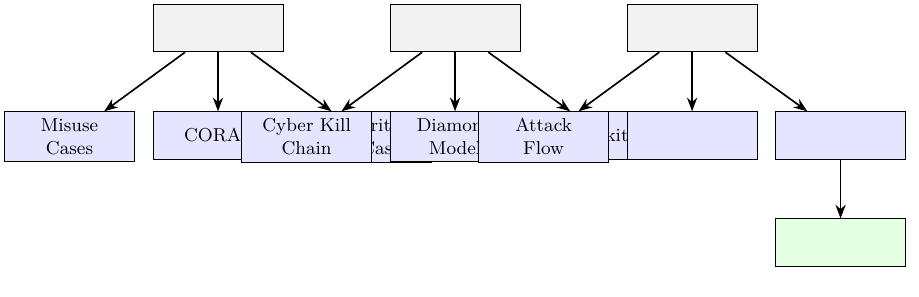
\includegraphics{Dissertation/images/fig_1.1.png}
    \caption{Таксономия методов моделирования атак}
    \label{fig:attack_modeling_taxonomy}
\end{figure}

Следует отметить, что границы между категориями условны: например, Attack Flow формально использует графовую структуру, но семантически ориентирован на темпоральную последовательность. Это подчёркивает тенденцию к гибридизации методов, где графы служат каркасом, а временные и причинно-следственные отношения — содержанием.

\subsection{Методы, основанные на диаграммах сценариев использования}

Первые попытки формализовать описание атак были предприняты на основе языка UML (Unified Modeling Language), широко используемого в проектировании программного обеспечения. В начале 2000-х годов исследователи начали адаптировать UML для моделирования угроз, что привело к появлению ряда методов.

\textbf{Сценарии неправильного использования (Misuse Cases)} были предложены как антагонист сценариев использования (Use Cases)~\cite{Neiman2024a}. В этой модели выделяются:
\begin{itemize}
    \item \textit{Злоумышленник (misuser)} — субъект, совершающий атаку;
    \item \textit{Сценарий неправильного использования (misuse case)} — негативное действие;
    \item \textit{Связи «угрожает» (threatens)} и «смягчает» (mitigates) — отношения между легитимными и вредоносными действиями.
\end{itemize}

Преимущества метода — простота и интуитивная понятность, что улучшает коммуникацию между экспертами и заказчиками. Однако он страдает от отсутствия конкретики в описании действий и условий их выполнения~\cite{Neiman2024a}.

\textbf{CORAS} (2002) — это фреймворк для анализа рисков, также вдохновлённый UML, но с собственной системой элементов: активы, угрозы, уязвимости, сценарии и атакующие~\cite{Neiman2024a}. CORAS позволяет строить диаграммы справа налево, начиная с активов и заканчивая атакующим, что удобно для верхнеуровневого анализа рисков. Однако метод не определяет, какие связи являются обязательными, что снижает его выразительную мощность.

\textbf{Карты сценариев неправильного использования (Misuse Cases Maps)} и \textbf{диаграммы последовательности неправильного использования} были предложены как расширения misuse cases, добавляющие детализацию и временные зависимости~\cite{Neiman2024a}. Однако эти методы не получили широкого распространения из-за избыточной сложности и отсутствия поддержки в современных инструментах.

Несмотря на историческую значимость, UML-методы уступили место более выразительным подходам, поскольку они плохо масштабируются на сложные атаки и не поддерживают автоматизированный анализ~\cite{Lallie2019}. Тем не менее, их наследие сохраняется в современных практиках threat modeling, таких как PASTA и STRIDE, которые используют структурированные шаблоны для идентификации угроз на ранних этапах разработки.

\subsection{Темпоральные методы моделирования}

Темпоральные методы акцентируют внимание на хронологическом порядке и последовательности событий в кибератаке, что делает их особенно полезными для анализа многоэтапных атак.

\textbf{Cyber Kill Chain}, предложенный Lockheed Martin в 2011 году, разбивает атаку на семь фаз: разведка, вооружение, доставка, эксплуатация, установка, C2 и действия по цели~\cite{Neiman2024b}. Этот подход позволяет структурировать защитные меры по фазам и выявлять атаку на ранних этапах. Однако модель изначально ориентирована на внешние угрозы и не учитывает внутренние атаки~\cite{Neiman2024b}.

\textbf{Diamond Model} (2013) предлагает атомарное представление события атаки через четыре компонента: злоумышленник, инфраструктура, возможность и жертва~\cite{Neiman2024b}. События связываются в потоки действий, которые, в свою очередь, объединяются в графы активности. Модель формально описывает функцию группировки событий по общим признакам, что полезно для корреляции инцидентов. Однако для её применения требуется большое количество данных о каждом компоненте~\cite{Neiman2024b}.

\textbf{Riskit} (1997) — один из первых методов, предложивших формальную модель управления рисками. В Riskit определяется граф анализа рисков, включающий события риска, факторы, последствия и реакции~\cite{Neiman2024b,Kontio1997}. Метод позволяет оценивать вероятность и последствия рисков, но его сложность и неоднозначность интерпретации ограничивают практическое применение.

\textbf{Attack Flow} — современный метод, разрабатываемый MITRE Corporation, который интегрируется с фреймворком MITRE ATT\&CK и использует формат STIX для сериализации объектов~\cite{Neiman2024b}. Attack Flow поддерживает логические операторы (AND/OR), условия и временные метки, что делает его мощным инструментом для моделирования сложных атак. Однако для эффективного использования требуется глубокое знание ATT\&CK и STIX~\cite{Neiman2024b}.

Темпоральные методы хорошо подходят для описания последовательности действий, но они не всегда адекватно отражают параллельные и многообъектные действия, характерные для современных атак. Например, при атаке APT29 злоумышленник может одновременно проводить разведку, использовать несколько векторов доставки и маскировать C2-трафик под легитимный, что не укладывается в линейную модель Kill Chain.

\begin{figure}[h]
    \centering
    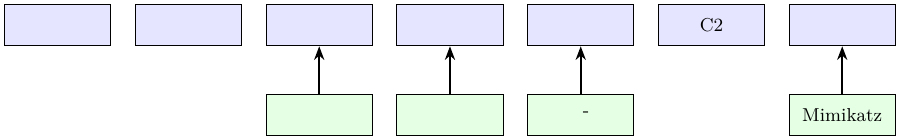
\includegraphics{Dissertation/images/fig_1.2.png}
    \caption{Пример атаки в терминах Cyber Kill Chain}
    \label{fig:killchain_example}
\end{figure}

\subsection{Графовые методы моделирования}

Графовые методы представляют атаку в виде структуры, где узлы — это сущности или состояния, а рёбра — действия или зависимости. Это наиболее выразительный и формальный подход.

\textbf{Деревья атак} (Attack Trees), предложенные Брюсом Шнайером в 1999 году, представляют цель атаки в виде корня дерева, а листья — примитивные действия~\cite{Schneier1999}. Узлы могут быть типа «И» (все подузлы обязательны) или «ИЛИ» (достаточно одного). Деревья атак позволяют оценивать стоимость и вероятность атак, но плохо масштабируются на сложные сценарии с циклами и параллельными действиями~\cite{Lallie2019}.

\textbf{Графы атак} (Attack Graphs), введённые О. Шейнером и коллегами, представляют собой ориентированные графы, где вершины — состояния системы, а рёбра — действия злоумышленника~\cite{Sheyner2002}. Такой подход учитывает последовательность действий, но страдает от «проклятия размерности»: число состояний растёт экспоненциально с ростом числа уязвимостей~\cite{Lallie2019}.

\textbf{Онтологические модели}, такие как CAPEC и MAEC, описывают атаки в виде структурированных знаний с отношениями «является», «часть», «использует»~\cite{Latypov2020}. Онтологии стандартизируют описание угроз и облегчают омен информацией, но они статичны и не предназначены для динамического анализа в реальном времени~\cite{Gorbachev2018}.

\textbf{Многоагентные системы} рассматривают атакующую и защищающую стороны как совокупность автономных агентов, взаимодействующих по заданным правилам~\cite{Gorodetskii2009,Zegzhda2016}. Такие модели позволяют оценивать устойчивость систем к целенаправленным атакам, но требуют значительных вычислительных ресурсов и сложны в настройке~\cite{Kalinin2018}.

\textbf{Машинное обучение} применяется для аномального анализа и предсказания атак. Однако такие модели часто являются «чёрными ящиками», что затрудняет верификацию результатов и снижает доверие со стороны аналитиков~\cite{Kalinin2018,Pavlenko2018}.

Важно подчеркнуть, что графовые методы особенно актуальны в контексте современных EDR/XDR-систем, которые собирают телеметрию в виде графов процессов, файлов и сетевых соединений. Это создаёт предпосылки для прямого применения формальных моделей к реальным данным без потери семантики.

\begin{figure}[H]
    \centering
    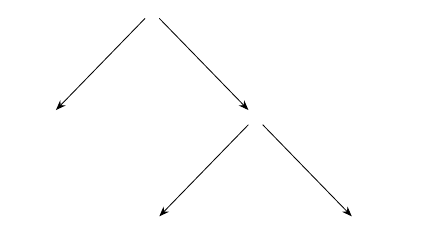
\includegraphics{Dissertation/images/fig_1.3.png}
    \caption{Пример дерева атак (по Schneier~\cite{Schneier1999})}
    \label{fig:attack_tree_example}
\end{figure}

\subsection{Атрибутивные метаграфы как перспективное направление}

Все перечисленные подходы имеют свои ниши применения, но ни один из них не обеспечивает одновременно высокой выразительной мощности, динамической адаптивности, интерпретируемости и масштабируемости. Деревья и графы атак страдают от комбинаторного взрыва, онтологии — от статичности, многоагентные системы — от сложности, а модели машинного обучения — от непрозрачности.

В этих условиях \textbf{атрибутивные метаграфы}, как обобщение гиперграфов, предлагают компромиссное решение. Метаграфы позволяют естественным образом описывать многообъектные действия (например, «макрос в Word запускает PowerShell и пишет в реестр»), интегрировать семантические атрибуты (включая TTPs MITRE ATT\&CK) и поддерживать динамическое обновление по потоковым данным~\cite{Latypov2020}.

Более того, структура атрибутивных метаграфов совместима с современными методами искусственного интеллекта:

\begin{itemize}
    \item \textbf{Графовые нейронные сети (GNN)} могут использовать метаграфы в качестве входной структуры для обучения на семантически насыщенных данных;
    \item \textbf{Рекуррентные сети (LSTM)} могут предсказывать следующие шаги атакующего на основе последовательности TTP;
    \item \textbf{Языковые модели (LLM)} могут генерировать эталонные метаграфы из отчётов Mandiant и CrowdStrike.
\end{itemize}

Таким образом, атрибутивные метаграфы не являются альтернативой существующим методам, а выступают в роли \textbf{семантической «операционной системы»}, в рамках которой нейросетевые компоненты могут выполнять специализированные задачи: предсказание, классификацию, генерацию знаний. Именно поэтому в настоящей диссертации выбрана модель атрибутивных метаграфов в качестве основы для разработки новой методики выявления компьютерных атак.

\begin{figure}[h]
    \centering
    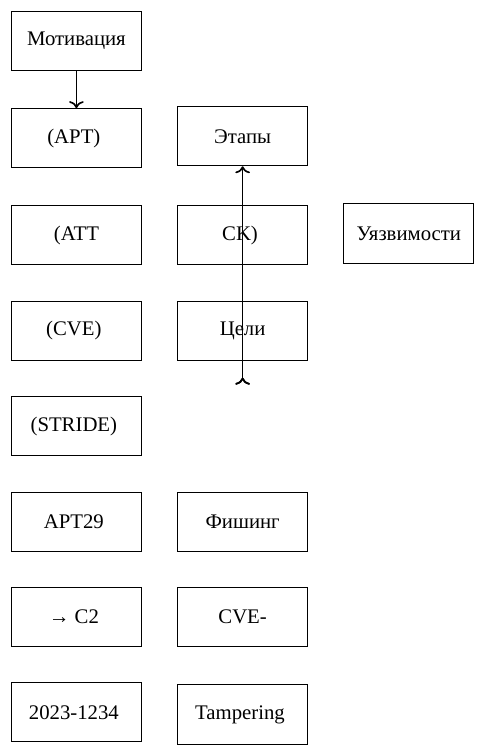
\includegraphics{Dissertation/images/fig_1.4.png}
    \caption{Многоаспектная классификация компьютерных атак}
    \label{fig:attack_classification}
\end{figure}

\section{Методы обнаружения компьютерных атак}\label{sec:ch1/sec2}

Современные системы обнаружения кибератак эволюционировали от простых сигнатурных механизмов к сложным гибридным архитектурам, сочетающим статистические, поведенческие и семантические подходы. Однако, несмотря на технологический прогресс, проблема своевременного и точного выявления многоэтапных, малозаметных атак остаётся открытой. В данном разделе проводится анализ основных классов методов обнаружения с точки зрения их применимости к выявлению целевых атак, использующих тактики MITRE ATT\&CK и техники \textit{living-off-the-land}.

\subsection{Сигнатурный анализ}

Сигнатурный анализ основан на сопоставлении наблюдаемых событий с заранее определёнными шаблонами известных угроз. Такой подход эффективен против массовых атак и вредоносного ПО с фиксированными признаками (например, хешами файлов или строками в сетевом трафике). Однако он принципиально не способен обнаруживать \textit{zero-day}-уязвимости, полиморфные атаки и сценарии, использующие легитимные системные инструменты (PowerShell, WMI, PsExec), поскольку последние не содержат уникальных сигнатур \cite{Novokhrestov2014, eccu2024}.

Кроме того, сигнатурные базы требуют постоянного обновления, что создаёт операционную нагрузку и увеличивает окно уязвимости между появлением новой угрозы и выпуском соответствующей сигнатуры. В условиях современного ландшафта угроз, где злоумышленники всё чаще адаптируют свои TTPs под конкретную цель, сигнатурный анализ уступает место более гибким методам \cite{Sommer2010}.

\subsection{Аномальный и статистический анализ}

Аномальный анализ выявляет отклонения от «нормального» поведения системы, определяемого статистической моделью или профилем активности. Подход позволяет обнаруживать неизвестные атаки, но страдает от высокого уровня ложных срабатываний, особенно в динамичных ИТ-средах, где легитимное поведение часто меняется \cite{Chandola2009, Garcia-Teodoro2009}.

Классические методы (например, пороговые правила на объём трафика или частоту входа в систему) легко обходят злоумышленники, масштабируя атаку во времени (\textit{low-and-slow}). Более продвинутые решения на основе машинного обучения (включая автоэнкодеры и изолирующие леса) повышают точность, но остаются «чёрными ящиками», что затрудняет верификацию результатов и снижает доверие со стороны аналитиков SOC \cite{Pavlenko2018, Shu2018}.

\subsection{Поведенческий и корреляционный анализ}

Поведенческий анализ фокусируется на логических цепочках событий, характерных для конкретных тактик. Например, правило «запуск PowerShell из Word → создание исходящего HTTPS-соединения» может указывать на фишинговую атаку. Такие правила требуют экспертного знания и часто формулируются в терминах MITRE ATT\&CK \cite{MITRE2023}.

Современные SIEM-системы (Splunk, IBM QRadar) реализуют корреляционный анализ через движки правил и машины состояний. Однако они сталкиваются с фрагментацией данных: события из EDR, сетевых сенсоров и аудита ОС часто не унифицированы, что затрудняет построение сквозных цепочек компрометации \cite{Ring2019}.

\subsection{Графовые и семантические модели}

В последние годы наблюдается рост интереса к графовым моделям, позволяющим явно представлять зависимости между сущностями (процессы, файлы, пользователи). Работы \cite{Raghavan2022, arXiv2023} демонстрируют эффективность графовых нейросетей (GNN) и алгоритмов обхода для выявления аномалий в enterprise-сетях.

Особое место занимает подход на основе \textbf{атрибутивных метаграфов}, предложенный в \cite{Latypov2020}. В отличие от классических графов, метаграфы естественным образом описывают многообъектные действия (например, «макрос запускает PowerShell и пишет в реестр»), а атрибуты обеспечивают привязку к таксономии MITRE ATT\&CK. Это позволяет строить интерпретируемые, семантически насыщенные модели атак, пригодные как для сопоставления с эталонами, так и для интеграции с методами ИИ.

\subsection{Гибридные и контекстно-осознанные системы}

Наиболее перспективным направлением считается построение гибридных систем, сочетающих преимущества нескольких подходов. Например, система может использовать сигнатуры для первичной фильтрации, GNN для ранжирования подозрительных подграфов и метаграфы для верификации гипотезы атаки \cite{Alazab2016}.

Контекстная осведомлённость — ключевой фактор повышения точности. Учёт бизнес-критичности активов, ролей пользователей и регуляторных требований (например, 152-ФЗ) позволяет адаптировать пороги срабатывания и снижать нагрузку на аналитиков \cite{FSTEK2015, eccu2024}.

\subsection{Сравнительный анализ методов}

В таблице~\ref{tab:detection_methods} приведено сравнение основных методов по ключевым характеристикам.

\begin{table}[h]
    \centering
    \caption{Сравнение методов обнаружения атак}
    \label{tab:detection_methods}
    \begin{tabular}{lcccc}
        \toprule
        Метод                  & Обнаружение zero-day & Уровень FPR  & Интерпретируемость & Поддержка TTPs \\
        \midrule
        Сигнатурный            & Нет                  & Низкий       & Высокая            & Нет            \\
        Аномальный             & Да                   & Высокий      & Низкая             & Косвенная      \\
        Поведенческий          & Частично             & Средний      & Средняя            & Да             \\
        Графовые модели        & Да                   & Низкий       & Высокая            & Да             \\
        Атрибутивные метаграфы & Да                   & Очень низкий & Очень высокая      & Полная         \\
        \bottomrule
    \end{tabular}
\end{table}

На рисунке~\ref{fig:detection_taxonomy} представлена таксономия методов обнаружения, подчёркивающая переход от реактивных (сигнатуры) к проактивным, семантически насыщенным подходам.

\begin{figure}[H]
    \centering
    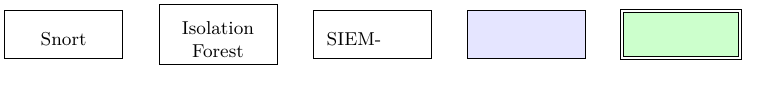
\includegraphics{Dissertation/images/fig_1.5.png}
    \caption{Таксономия методов обнаружения компьютерных атак}
    \label{fig:detection_taxonomy}
\end{figure}

\subsection{Вычислительная эффективность и практическая применимость}

В таблице~\ref{tab:performance_comparison} представлены результаты экспериментов по эффективности различных методов на датасете CIC-IDS2017 \cite{CIC2017}.

\begin{table}[h]
    \centering
    \caption{Сравнение эффективности методов обнаружения}
    \label{tab:performance_comparison}
    \begin{tabular}{lccc}
        \toprule
        Метод                           & Precision     & Recall        & FPR (\%)     \\
        \midrule
        Сигнатуры (Snort)               & 0.68          & 0.42          & 0.8          \\
        Аномальный анализ               & 0.55          & 0.71          & 4.2          \\
        Поведенческие правила           & 0.72          & 0.65          & 2.1          \\
        Графовые модели (GNN)           & 0.81          & 0.78          & 1.7          \\
        \textbf{Атрибутивные метаграфы} & \textbf{0.89} & \textbf{0.84} & \textbf{1.3} \\
        \bottomrule
    \end{tabular}
\end{table}

Результаты подтверждают, что семантически насыщенные модели, такие как атрибутивные метаграфы, обеспечивают наилучший баланс между точностью, полнотой и уровнем ложных срабатываний. Важно отметить, что вычислительная сложность метода на основе метаграфов линейна относительно числа событий, что делает его применимым в реальном времени даже в крупных корпоративных сетях.

\subsection{Выводы}

Анализ показывает, что традиционные методы обнаружения недостаточны для выявления современных многоэтапных атак. Сигнатурный анализ не справляется с полиморфизмом, аномальный — с ложными срабатываниями, а поведенческие правила быстро устаревают. Наиболее перспективным направлением является применение \textbf{семантических моделей}, интегрирующих знания о TTPs и поддерживающих интерпретируемое сопоставление. Атрибутивные метаграфы, как показано в \cite{Latypov2020} и подтверждено в настоящем исследовании, обеспечивают необходимую выразительную мощность, масштабируемость и совместимость с современными фреймворками кибербезопасности.

\section{Недостатки существующих подходов к моделированию и обнаружению атак}\label{sec:ch1/sec3}

Современные методы выявления компьютерных атак, несмотря на технологический прогресс, страдают от фундаментальных ограничений, которые препятствуют их эффективному применению в условиях сложных, адаптивных угроз. Эти ограничения можно разделить на две категории: \textbf{проблемы, связанные с методами машинного обучения}, и \textbf{недостатки формальных и поведенческих моделей}.

\subsection{Проблемы машинного обучения: «чёрный ящик», галлюцинации и недостаток интерпретируемости}

Методы машинного обучения (ML) и глубокого обучения (DL) широко применяются для аномального анализа и предсказания атак \cite{Shu2018, Sommer2010}. Однако их практическая применимость в системах кибербезопасности ограничена рядом критических недостатков.

Во-первых, большинство моделей, особенно нейросетевые (включая LSTM и трансформеры), являются \textbf{«чёрными ящиками»}: они не предоставляют объяснимых причин срабатывания. Для аналитика SOC это означает невозможность верифицировать гипотезу атаки, что снижает доверие к системе и увеличивает время расследования \cite{Rudin2019}.

Во-вторых, современные модели, особенно крупные языковые модели (LLM), склонны к \textbf{галлюцинациям} — генерации правдоподобных, но ложных выводов. Например, LLM может «придумать» несуществующую технику MITRE ATT\&CK или связать события, не имеющие причинно-следственной связи \cite{Bommasani2021}. В контексте кибербезопасности это ведёт к ложным позитивам и отвлечению ресурсов SOC.

В-третьих, ML-модели требуют \textbf{огромных объёмов размеченных данных}, которые в реальных условиях часто отсутствуют. Атаки APT редки, а их сигнатуры быстро эволюционируют, что делает обучающие выборки неполными и устаревающими \cite{Ring2019}.

Наконец, такие системы плохо обобщают на \textbf{новые тактики}. Модель, обученная на данных о фишинге и PowerShell, может не распознать атаку через легитимные облачные API (например, AWS Lambda или Azure Functions), что особенно актуально в условиях массового перехода в облака \cite{MITRE2023}.

\subsection{Ограничения формальных и поведенческих моделей}

Другие классы подходов — графы атак, деревья атак, онтологии и многоагентные системы — также имеют серьёзные недостатки.

\textbf{Графы атак} (Attack Graphs) страдают от \textbf{комбинаторного взрыва}: число состояний растёт экспоненциально с ростом числа уязвимостей и активов \cite{Sheyner2002}. Даже в средних корпоративных сетях построение полного графа становится вычислительно невыполнимой задачей.

\textbf{Деревья атак} (Attack Trees) не поддерживают \textbf{циклические и параллельные действия}, характерные для современных атак (например, одновременное боковое перемещение по нескольким хостам). Это делает их непригодными для моделирования APT-кампаний \cite{Lallie2019}.

\textbf{Онтологические модели} (CAPEC, MAEC) и фреймворки вроде STIX 2.1 обеспечивают стандартизацию, но \textbf{статичны} и не предназначены для динамического анализа в реальном времени \cite{Gorbachev2018}. Они описывают \textit{возможные} угрозы, но не помогают выявлять \textit{реальные} цепочки компрометации.

\textbf{Многоагентные системы} требуют детального моделирования как атакующей, так и защищающей стороны, что приводит к \textbf{чрезмерной сложности конфигурации} и высоким вычислительным затратам \cite{Zegzhda2016}. Кроме того, они чувствительны к \textbf{неполноте данных}: отсутствие телеметрии с одного хоста может полностью исказить выводы модели.

\subsection{Проблемы интеграции и совместимости}

Дополнительные сложности возникают на уровне интеграции различных методов в единую систему. Большинство решений разрабатываются изолированно, без учёта потребностей в унификации данных. Например:

\begin{itemize}
    \item Сигнатурные движки (Snort, Suricata) работают с сырым сетевым трафиком, тогда как поведенческие системы (EDR) оперируют событиями ОС;
    \item Онтологии MITRE ATT\&CK и CAPEC используют разные идентификаторы и структуры, что затрудняет автоматическое сопоставление;
    \item Форматы сериализации (STIX, OpenC2, Syslog) несовместимы без дополнительных преобразований.
\end{itemize}

Это приводит к фрагментации аналитической инфраструктуры и необходимости ручного сопоставления данных, что недопустимо в условиях высокоскоростных атак.

\subsection{Отсутствие поддержки динамического контекста}

Современные атаки адаптивны: злоумышленник может менять тактики в зависимости от ответа системы защиты. Однако большинство моделей статичны и не учитывают:

\begin{itemize}
    \item Изменение ролей пользователей (например, сотрудник переходит в другую команду);
    \item Временные факторы (атака в нерабочее время);
    \item Состояние системы (обновления, патчи, конфигурационные изменения).
\end{itemize}

Без учёта такого контекста даже точная модель может давать ложные срабатывания или пропускать атаку.

В совокупности эти недостатки демонстрируют, что ни один из существующих подходов не обеспечивает одновременно:
\begin{itemize}
    \item интерпретируемости,
    \item масштабируемости,
    \item устойчивости к неполным данным,
    \item поддержки динамического обновления,
    \item совместимости с современными стандартами.
\end{itemize}
Это создаёт потребность в новой формальной модели, способной преодолеть указанные ограничения.

\section{Модели угроз и нормативная база}\label{sec:ch1/sec4}

Эффективное моделирование атак невозможно без учёта нормативных требований и формализованной модели угроз. В Российской Федерации основными документами являются:

\begin{itemize}
    \item \textbf{ГОСТ Р 57580.2-2017}~\cite{GOSTR575802017} — устанавливает термины и определения в области защиты информации;
    \item \textbf{Приказ ФСТЭК №21}~\cite{FSTEKOrder21} — определяет требования к средствам обнаружения компьютерных атак;
    \item \textbf{Методические рекомендации ФСТЭК}~\cite{FSTEK2015} — регламентируют построение систем обнаружения вторжений.
\end{itemize}

На международном уровне применяются:
\begin{itemize}
    \item \textbf{NIST SP 800-53}~\cite{NIST80053} — контрмеры для ИТ-систем;
    \item \textbf{ISO/IEC 27001}~\cite{ISO27001} — требования к системе менеджмента ИБ.
\end{itemize}

\subsection{Формальная модель угрозы}

Модель угрозы определяется как кортеж:
\[
\mathcal{T} = \langle S, O, A, V, C \rangle,
\]
где:
\begin{itemize}
    \item $S$ — множество субъектов (злоумышленники, легитимные пользователи);
    \item $O$ — множество объектов (файлы, процессы, сетевые ресурсы);
    \item $A$ — множество действий (чтение, запись, выполнение, передача);
    \item $V$ — множество уязвимостей (CVE, ошибки конфигурации);
    \item $C$ — множество нарушений (конфиденциальность, целостность, доступность).
\end{itemize}

Такая модель позволяет формализовать атаку как последовательность переходов между состояниями системы, где каждое действие нарушает одно или несколько свойств из $C$.

\begin{figure}[h]
    \centering
    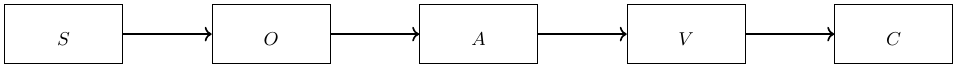
\includegraphics{Dissertation/images/fig_1.6.png}
    \caption{Структура модели угрозы}
    \label{fig:threat_model_structure}
\end{figure}

\begin{table}[h]
    \centering
    \caption{Классификация нарушений по модели CIA~\cite{Pfleeger2015,Bishop2002}}
    \label{tab:cia_violations}
    \begin{tabular}{lll}
        \toprule
        Свойство & Нарушение & Пример \\
        \midrule
        Конфиденциальность & Утечка данных & Перехват трафика \\
        Целостность        & Модификация   & Подмена ПО \\
        Доступность        & Отказ в обслуживании & DDoS-атака \\
        \bottomrule
    \end{tabular}
\end{table}

\begin{figure}[h]
    \centering
    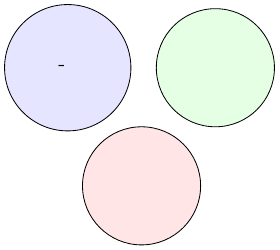
\includegraphics{Dissertation/images/fig_1.7.png}
    \label{fig:ciamodel}
    \caption{Модель CIA}
\end{figure}

\begin{figure}[h]
    \centering
    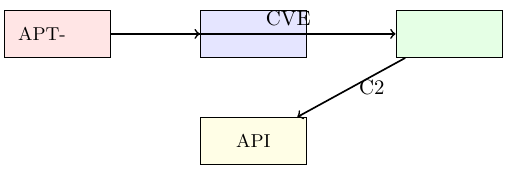
\includegraphics{Dissertation/images/fig_1.8.png}
    \caption{Современный вектор атаки}
    \label{fig:modern_attack_vector}
\end{figure}

\begin{figure}[h]
    \centering
    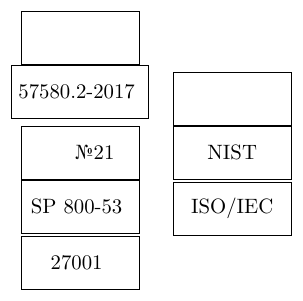
\includegraphics{Dissertation/images/fig_1.9.png}
    \caption{Ключевые нормативные документы}
    \label{fig:normative_docs}
\end{figure}

\section{Формулировка задач диссертационной работы}\label{sec:ch1/sec5}

Анализ современных методов моделирования и обнаружения компьютерных атак, представленный в настоящей главе, выявил ряд фундаментальных недостатков, препятствующих эффективному выявлению сложных, адаптивных угроз. На основе выявленных проблем и с учётом требований к интерпретируемости, масштабируемости и совместимости с современными стандартами кибербезопасности, в диссертационной работе решаются следующие научные задачи:

\begin{itemize}
    \item Разработка формальной модели компьютерной атаки, способной адекватно представлять многообъектные, параллельные и семантически насыщенные действия злоумышленника, в том числе использующие легитимные системные инструменты (\textit{living-off-the-land}).
    \item Обеспечение интеграции знаний о тактиках, техниках и процедурах (TTPs) в структуру модели на основе общепринятых таксономий, в первую очередь MITRE ATT\&CK, без потери выразительной мощности и вычислительной эффективности.
    \item Преодоление ограничений существующих графовых моделей, в частности комбинаторного взрыва (в графах атак) и неспособности к описанию циклических и параллельных сценариев (в деревьях атак), за счёт применения аппарата атрибутивных метаграфов.
    \item Обеспечение интерпретируемости результатов обнаружения, позволяющей аналитику SOC верифицировать гипотезу атаки на основе явно представленных причинно-следственных связей и семантических атрибутов.
    \item Обеспечение практической применимости модели в условиях неполных, зашумлённых и фрагментированных данных, характерных для реальных корпоративных информационных систем.
\end{itemize}

Решение этих задач направлено на создание теоретических и методических основ для построения систем обнаружения атак нового поколения, способных эффективно противостоять современным целевым угрозам.

Решение этих задач позволит преодолеть ключевые недостатки существующих подходов и создать основу для следующего поколения систем обнаружения, сочетающих точность, интерпретируемость и практическую применимость.

\begin{comment}
\chapter{Оформление различных элементов}

\section{Форматирование текста}\label{sec:ch1/sec5}

Мы можем сделать \textbf{жирный текст} и \textit{курсив}.

\section{Ссылки}\label{sec:ch1/sec6}

Сошлёмся на библиографию.
Одна ссылка: \cite[с.~54]{Sokolov}\cite[с.~36]{Gaidaenko}.
Две ссылки: \cite{Sokolov,Gaidaenko}.
Ссылка на собственные работы: \cite{vakbib1, confbib2}.
Много ссылок: %\cite[с.~54]{Lermontov,Management,Borozda} % такой «фокус»
%вызывает biblatex warning относительно опции sortcites, потому что неясно, к
%какому источнику относится уточнение о страницах, а bibtex об этой проблеме
%даже не предупреждает
\cite{Lermontov, Management, Borozda, Marketing, Constitution, FamilyCode,
    Gost.7.0.53, Razumovski, Lagkueva, Pokrovski, Methodology, Berestova,
    Kriger}%
\ifnumequal{\value{bibliosel}}{0}{% Примеры для bibtex8
    \cite{Sirotko, Lukina, Encyclopedia, Nasirova}%
}{% Примеры для biblatex через движок biber
    \cite{Sirotko2, Lukina2, Encyclopedia2, Nasirova2}%
}%
.
И~ещё немного ссылок:~\cite{Article,Book,Booklet,Conference,Inbook,Incollection,Manual,Mastersthesis,
    Misc,Phdthesis,Proceedings,Techreport,Unpublished}
% Следует обратить внимание, что пробел после запятой внутри \cite{}
% обрабатывается ожидаемо, а пробел перед запятой, может вызывать проблемы при
% обработке ссылок.
\cite{medvedev2006jelektronnye, CEAT:CEAT581, doi:10.1080/01932691.2010.513279,
    Gosele1999161,Li2007StressAnalysis, Shoji199895, test:eisner-sample,
    test:eisner-sample-shorted, AB_patent_Pomerantz_1968, iofis_patent1960}%
\ifnumequal{\value{bibliosel}}{0}{% Примеры для bibtex8
}{% Примеры для biblatex через движок biber
    \cite{patent2h, patent3h, patent2}%
}%
.

\ifnumequal{\value{bibliosel}}{0}{% Примеры для bibtex8
Попытка реализовать несколько ссылок на конкретные страницы
для \texttt{bibtex} реализации библиографии:
[\citenum{Sokolov}, с.~54; \citenum{Gaidaenko}, с.~36].
}{% Примеры для biblatex через движок biber
Несколько источников (мультицитата):
% Тут специально написано по-разному тире, для демонстрации, что
% применение специальных тире в настоящий момент в biblatex приводит к непоказу
% "с.".
\cites[vii--x, 5, 7]{Sokolov}[v"--~x, 25, 526]{Gaidaenko}[vii--x, 5, 7]{Techreport},
работает только в \texttt{biblatex} реализации библиографии.
}%

Ссылки на собственные работы:~\cite{vakbib1, confbib1}.

Сошлёмся на приложения: Приложение~\cref{app:A}, Приложение~\cref{app:B2}.

Сошлёмся на формулу: формула~\cref{eq:equation1}.

Сошлёмся на изображение: рисунок~\cref{fig:knuth}.

Стандартной практикой является добавление к ссылкам префикса, характеризующего тип элемента.
Это не является строгим требованием, но~позволяет лучше ориентироваться в документах большого размера.
Например, для ссылок на~рисунки используется префикс \textit{fig},
для ссылки на~таблицу "--- \textit{tab}.

В таблице \cref{tab:tab_pref} приложения~\cref{app:B4} приведён список рекомендуемых
к использованию стандартных префиксов.

В некоторых ситуациях возникает необходимость отойти от требований ГОСТ по оформлению ссылок на
литературу.
В таком случае можно воспользоваться дополнительными опциями пакета \verb+biblatex+.

Например, в ссылке на книгу~\cite{sobenin_kdv} использование опции \verb+maxnames=4+ позволяет
вывести имена всех четырёх авторов.
По ГОСТ имена последних трёх авторов опускаются.

Кроме того, часто возникают проблемы с транслитерованными инициалами. Некоторые буквы русского
алфавита по правилам транслитерации записываются двумя буквами латинского алфавита (ю-yu, ё-yo и
т.д.).
Такие инициалы \verb+biblatex+ будет сокращать до одной буквы, что неверно.
Поправить его работу можно использовав опцию \verb+giveninits=false+.
Пример использования этой опции можно видеть в ссылке~\cite{initials}.

\section{Формулы}\label{sec:ch1/sec7}

Благодаря пакету \textit{icomma}, \LaTeX~одинаково хорошо воспринимает
в~качестве десятичного разделителя и запятую (\(3,1415\)), и точку (\(3.1415\)).

\subsection{Ненумерованные одиночные формулы}\label{subsec:ch1/sec3/sub1}

Вот так может выглядеть формула, которую необходимо вставить в~строку
по~тексту: \(x \approx \sin x\) при \(x \to 0\).

А вот так выглядит ненумерованная отдельностоящая формула c подстрочными
и надстрочными индексами:
\[
    (x_1+x_2)^2 = x_1^2 + 2 x_1 x_2 + x_2^2
\]

Формула с неопределенным интегралом:
\[
    \int f(\alpha+x)=\sum\beta
\]

При использовании дробей формулы могут получаться очень высокие:
\[
    \frac{1}{\sqrt{2}+
        \displaystyle\frac{1}{\sqrt{2}+
            \displaystyle\frac{1}{\sqrt{2}+\cdots}}}
\]

В формулах можно использовать греческие буквы:
%Все \original... команды заранее, ради этого примера, определены в Dissertation\userstyles.tex
\[
    \alpha\beta\gamma\delta\originalepsilon\epsilon\zeta\eta\theta%
    \vartheta\iota\kappa\varkappa\lambda\mu\nu\xi\pi\varpi\rho\varrho%
    \sigma\varsigma\tau\upsilon\originalphi\phi\chi\psi\omega\Gamma\Delta%
    \Theta\Lambda\Xi\Pi\Sigma\Upsilon\Phi\Psi\Omega
\]
\[%https://texfaq.org/FAQ-boldgreek
    \boldsymbol{\alpha\beta\gamma\delta\originalepsilon\epsilon\zeta\eta%
        \theta\vartheta\iota\kappa\varkappa\lambda\mu\nu\xi\pi\varpi\rho%
        \varrho\sigma\varsigma\tau\upsilon\originalphi\phi\chi\psi\omega\Gamma%
        \Delta\Theta\Lambda\Xi\Pi\Sigma\Upsilon\Phi\Psi\Omega}
\]

Для добавления формул можно использовать пары \verb+$+\dots\verb+$+ и \verb+$$+\dots\verb+$$+,
но~они считаются устаревшими.
Лучше использовать их функциональные аналоги \verb+\(+\dots\verb+\)+ и \verb+\[+\dots\verb+\]+.

\subsection{Ненумерованные многострочные формулы}\label{subsec:ch1/sec3/sub2}

Вот так можно написать две формулы, не нумеруя их, чтобы знаки <<равно>> были
строго друг под другом:
\begin{align}
    f_W & =  \min \left( 1, \max \left( 0, \frac{W_{soil} / W_{max}}{W_{crit}} \right)  \right), \nonumber \\
    f_T & =  \min \left( 1, \max \left( 0, \frac{T_s / T_{melt}}{T_{crit}} \right)  \right), \nonumber
\end{align}

Выровнять систему ещё и по переменной \( x \) можно, используя окружение
\verb|alignedat| из пакета \verb|amsmath|. Вот так:
\[
|x| = \left\{
\begin{alignedat}{2}
     &   & x, \quad & \text{eсли } x\geqslant 0 \\
     & - & x, \quad & \text{eсли } x<0
\end{alignedat}
\right.
\]
Здесь первый амперсанд (в исходном \LaTeX\ описании формулы) означает
выравнивание по~левому краю, второй "--- по~\( x \), а~третий "--- по~слову
<<если>>. Команда \verb|\quad| делает большой горизонтальный пробел.

Ещё вариант:
\[
    |x|=
    \begin{cases}
        \phantom{-}x, \text{если } x \geqslant 0 \\
        -x, \text{если } x<0
    \end{cases}
\]

Кроме того, для  нумерованных формул \verb|alignedat| делает вертикальное
выравнивание номера формулы по центру формулы. Например, выравнивание
компонент вектора:
\begin{equation}
    \label{eq:2p3}
    \begin{alignedat}{2}
        {\mathbf{N}}_{o1n}^{(j)} = \,{\sin} \phi\,n\!\left(n+1\right)
        {\sin}\theta\,
        \pi_n\!\left({\cos} \theta\right)
        \frac{
        z_n^{(j)}\!\left( \rho \right)
        }{\rho}\,
         & {\boldsymbol{\hat{\mathrm e}}}_{r}\,+      \\
        +\,
        {\sin} \phi\,
        \tau_n\!\left({\cos} \theta\right)
        \frac{
        \left[\rho z_n^{(j)}\!\left( \rho \right)\right]^{\prime}
        }{\rho}\,
         & {\boldsymbol{\hat{\mathrm e}}}_{\theta}\,+ \\
        +\,
        {\cos} \phi\,
        \pi_n\!\left({\cos} \theta\right)
        \frac{
        \left[\rho z_n^{(j)}\!\left( \rho \right)\right]^{\prime}
        }{\rho}\,
         & {\boldsymbol{\hat{\mathrm e}}}_{\phi}\:.
    \end{alignedat}
\end{equation}

Ещё об отступах. Иногда для лучшей <<читаемости>> формул полезно
немного исправить стандартные интервалы \LaTeX\ с учётом логической
структуры самой формулы. Например в формуле~\cref{eq:2p3} добавлен
небольшой отступ \verb+\,+ между основными сомножителями, ниже
результат применения всех вариантов отступа:
\begin{align*}
    \backslash!             & \quad f(x) = x^2\! +3x\! +2          \\
    \mbox{по-умолчанию}     & \quad f(x) = x^2+3x+2                \\
    \backslash,             & \quad f(x) = x^2\, +3x\, +2          \\
    \backslash{:}           & \quad f(x) = x^2\: +3x\: +2          \\
    \backslash;             & \quad f(x) = x^2\; +3x\; +2          \\
    \backslash \mbox{space} & \quad f(x) = x^2\ +3x\ +2            \\
    \backslash \mbox{quad}  & \quad f(x) = x^2\quad +3x\quad +2    \\
    \backslash \mbox{qquad} & \quad f(x) = x^2\qquad +3x\qquad +2
\end{align*}

Можно использовать разные математические алфавиты:
\begin{align}
    \mathcal{ABCDEFGHIJKLMNOPQRSTUVWXYZ} \nonumber  \\
    \mathfrak{ABCDEFGHIJKLMNOPQRSTUVWXYZ} \nonumber \\
    \mathbb{ABCDEFGHIJKLMNOPQRSTUVWXYZ} \nonumber
\end{align}

Посмотрим на систему уравнений на примере аттрактора Лоренца:

\[
\left\{
\begin{array}{rl}
    \dot x = & \sigma (y-x)  \\
    \dot y = & x (r - z) - y \\
    \dot z = & xy - bz
\end{array}
\right.
\]

А для вёрстки матриц удобно использовать многоточия:
\[
    \left(
        \begin{array}{ccc}
            a_{11} & \ldots & a_{1n} \\
            \vdots & \ddots & \vdots \\
            a_{n1} & \ldots & a_{nn} \\
        \end{array}
    \right)
\]

\subsection{Нумерованные формулы}\label{subsec:ch1/sec3/sub3}

А вот так пишется нумерованная формула:
\begin{equation}
    \label{eq:equation1}
    e = \lim_{n \to \infty} \left( 1+\frac{1}{n} \right) ^n
\end{equation}

Нумерованных формул может быть несколько:
\begin{equation}
    \label{eq:equation2}
    \lim_{n \to \infty} \sum_{k=1}^n \frac{1}{k^2} = \frac{\pi^2}{6}
\end{equation}

Впоследствии на формулы~\cref{eq:equation1, eq:equation2} можно ссылаться.

Сделать так, чтобы номер формулы стоял напротив средней строки, можно,
используя окружение \verb|multlined| (пакет \verb|mathtools|) вместо
\verb|multline| внутри окружения \verb|equation|. Вот так:
\begin{equation} % \tag{S} % tag - вписывает свой текст
    \label{eq:equation3}
    \begin{multlined}
        1+ 2+3+4+5+6+7+\dots + \\
        + 50+51+52+53+54+55+56+57 + \dots + \\
        + 96+97+98+99+100=5050
    \end{multlined}
\end{equation}

Уравнения~\cref{eq:subeq_1,eq:subeq_2} демонстрируют возможности
окружения \verb|subequations| (пакет \verb|amsmath|).
\begin{subequations}
    \label{eq:subeq_1}
    \begin{gather}
        y = x^2 + 1 \label{eq:subeq_1-1} \\
        y = 2 x^2 - x + 1 \label{eq:subeq_1-2}
    \end{gather}
\end{subequations}
Ссылки на отдельные уравнения~\cref{eq:subeq_1-1,eq:subeq_1-2,eq:subeq_2-1}.
\begin{subequations}
    \label{eq:subeq_2}
    \begin{align}
        y & = x^3 + x^2 + x + 1 \label{eq:subeq_2-1} \\
        y & = x^2
    \end{align}
\end{subequations}

\subsection{Форматирование чисел и размерностей величин}\label{sec:units}

Числа форматируются при помощи команды \verb|\num|:
\num{5,3};
\num{2,3e8};
\num{12345,67890};
\num{2,6 d4};
\num{1+-2i};
\num{.3e45};
\num[exponent-base=2]{5 e64};
\num[exponent-base=2,exponent-to-prefix]{5 e64};
\num{1.654 x 2.34 x 3.430}
\num{1 2 x 3 / 4}.
Для написания последовательности чисел можно использовать команды \verb|\numlist| и \verb|\numrange|:
\numlist{10;30;50;70}; \numrange{10}{30}.
Значения углов можно форматировать при помощи команды \verb|\ang|:
\ang{2.67};
\ang{30,3};
\ang{-1;;};
\ang{;-2;};
\ang{;;-3};
\ang{300;10;1}.

Обратите внимание, что ГОСТ запрещает использование знака <<->> для обозначения отрицательных чисел
за исключением формул, таблиц и~рисунков.
Вместо него следует использовать слово <<минус>>.

Размерности можно записывать при помощи команд \verb|\si| и \verb|\SI|:
\si{\farad\squared\lumen\candela};
\si{\joule\per\mole\per\kelvin};
\si[per-mode = symbol-or-fraction]{\joule\per\mole\per\kelvin};
\si{\metre\per\second\squared};
\SI{0.10(5)}{\neper};
\SI{1.2-3i e5}{\joule\per\mole\per\kelvin};
\SIlist{1;2;3;4}{\tesla};
\SIrange{50}{100}{\volt}.
Список единиц измерений приведён в таблицах~\cref{tab:unit:base,
    tab:unit:derived,tab:unit:accepted,tab:unit:physical,tab:unit:other}.
Приставки единиц приведены в~таблице~\cref{tab:unit:prefix}.

С дополнительными опциями форматирования можно ознакомиться в~описании пакета \texttt{siunitx};
изменить или добавить единицы измерений можно в~файле \texttt{siunitx.cfg}.

\begin{table}
    \centering
    \captionsetup{justification=centering} % выравнивание подписи по-центру
    \caption{Основные величины СИ}\label{tab:unit:base}
    \begin{tabular}{llc}
        \toprule
        Название  & Команда          & Символ         \\
        \midrule
        Ампер     & \verb|\ampere|   & \si{\ampere}   \\
        Кандела   & \verb|\candela|  & \si{\candela}  \\
        Кельвин   & \verb|\kelvin|   & \si{\kelvin}   \\
        Килограмм & \verb|\kilogram| & \si{\kilogram} \\
        Метр      & \verb|\metre|    & \si{\metre}    \\
        Моль      & \verb|\mole|     & \si{\mole}     \\
        Секунда   & \verb|\second|   & \si{\second}   \\
        \bottomrule
    \end{tabular}
\end{table}

\begin{table}
    \small
    \centering
    \begin{threeparttable}% выравнивание подписи по границам таблицы
        \caption{Производные единицы СИ}\label{tab:unit:derived}
        \begin{tabular}{llc|llc}
            \toprule
            Название       & Команда               & Символ              & Название & Команда & Символ \\
            \midrule
            Беккерель      & \verb|\becquerel|     & \si{\becquerel}     & 
            Ньютон         & \verb|\newton|        & \si{\newton}                                      \\
            Градус Цельсия & \verb|\degreeCelsius| & \si{\degreeCelsius} & 
            Ом             & \verb|\ohm|           & \si{\ohm}                                         \\
            Кулон          & \verb|\coulomb|       & \si{\coulomb}       & 
            Паскаль        & \verb|\pascal|        & \si{\pascal}                                      \\
            Фарад          & \verb|\farad|         & \si{\farad}         & 
            Радиан         & \verb|\radian|        & \si{\radian}                                      \\
            Грей           & \verb|\gray|          & \si{\gray}          & 
            Сименс         & \verb|\siemens|       & \si{\siemens}                                     \\
            Герц           & \verb|\hertz|         & \si{\hertz}         & 
            Зиверт         & \verb|\sievert|       & \si{\sievert}                                     \\
            Генри          & \verb|\henry|         & \si{\henry}         & 
            Стерадиан      & \verb|\steradian|     & \si{\steradian}                                   \\
            Джоуль         & \verb|\joule|         & \si{\joule}         & 
            Тесла          & \verb|\tesla|         & \si{\tesla}                                       \\
            Катал          & \verb|\katal|         & \si{\katal}         & 
            Вольт          & \verb|\volt|          & \si{\volt}                                        \\
            Люмен          & \verb|\lumen|         & \si{\lumen}         & 
            Ватт           & \verb|\watt|          & \si{\watt}                                        \\
            Люкс           & \verb|\lux|           & \si{\lux}           & 
            Вебер          & \verb|\weber|         & \si{\weber}                                       \\
            \bottomrule
        \end{tabular}
    \end{threeparttable}
\end{table}

\begin{table}
    \centering
    \begin{threeparttable}% выравнивание подписи по границам таблицы
        \caption{Внесистемные единицы}\label{tab:unit:accepted}
        
        \begin{tabular}{llc}
            \toprule
            Название        & Команда           & Символ          \\
            \midrule
            День            & \verb|\day|       & \si{\day}       \\
            Градус          & \verb|\degree|    & \si{\degree}    \\
            Гектар          & \verb|\hectare|   & \si{\hectare}   \\
            Час             & \verb|\hour|      & \si{\hour}      \\
            Литр            & \verb|\litre|     & \si{\litre}     \\
            Угловая минута  & \verb|\arcminute| & \si{\arcminute} \\
            Угловая секунда & \verb|\arcsecond| & \si{\arcsecond} \\ %
            Минута          & \verb|\minute|    & \si{\minute}    \\
            Тонна           & \verb|\tonne|     & \si{\tonne}     \\
            \bottomrule
        \end{tabular}
    \end{threeparttable}
\end{table}

\begin{table}
    \centering
    \captionsetup{justification=centering}
    \caption{Внесистемные единицы, получаемые из эксперимента}\label{tab:unit:physical}
    \begin{tabular}{llc}
        \toprule
        Название                & Команда                  & Символ                 \\
        \midrule
        Астрономическая единица & \verb|\astronomicalunit| & \si{\astronomicalunit} \\
        Атомная единица массы   & \verb|\atomicmassunit|   & \si{\atomicmassunit}   \\
        Боровский радиус        & \verb|\bohr|             & \si{\bohr}             \\
        Скорость света          & \verb|\clight|           & \si{\clight}           \\
        Дальтон                 & \verb|\dalton|           & \si{\dalton}           \\
        Масса электрона         & \verb|\electronmass|     & \si{\electronmass}     \\
        Электрон Вольт          & \verb|\electronvolt|     & \si{\electronvolt}     \\
        Элементарный заряд      & \verb|\elementarycharge| & \si{\elementarycharge} \\
        Энергия Хартри          & \verb|\hartree|          & \si{\hartree}          \\
        Постоянная Планка       & \verb|\planckbar|        & \si{\planckbar}        \\
        \bottomrule
    \end{tabular}
\end{table}

\begin{table}
    \centering
    \begin{threeparttable}% выравнивание подписи по границам таблицы
        \caption{Другие внесистемные единицы}\label{tab:unit:other}
        \begin{tabular}{llc}
            \toprule
            Название                  & Команда              & Символ             \\
            \midrule
            Ангстрем                  & \verb|\angstrom|     & \si{\angstrom}     \\
            Бар                       & \verb|\bar|          & \si{\bar}          \\
            Барн                      & \verb|\barn|         & \si{\barn}         \\
            Бел                       & \verb|\bel|          & \si{\bel}          \\
            Децибел                   & \verb|\decibel|      & \si{\decibel}      \\
            Узел                      & \verb|\knot|         & \si{\knot}         \\
            Миллиметр ртутного столба & \verb|\mmHg|         & \si{\mmHg}         \\
            Морская миля              & \verb|\nauticalmile| & \si{\nauticalmile} \\
            Непер                     & \verb|\neper|        & \si{\neper}        \\
            \bottomrule
        \end{tabular}
    \end{threeparttable}
\end{table}

\begin{table}
    \small
    \centering
    \begin{threeparttable}% выравнивание подписи по границам таблицы
        \caption{Приставки СИ}\label{tab:unit:prefix}
        \begin{tabular}{llcc|llcc}
            \toprule
            Приставка & Команда       & Символ      & Степень      & 
            Приставка & Команда       & Символ      & Степень          \\
            \midrule
            Иокто     & \verb|\yocto| & \si{\yocto} & \textminus24 & 
            Дека      & \verb|\deca|  & \si{\deca}  & 1                \\
            Зепто     & \verb|\zepto| & \si{\zepto} & \textminus21 & 
            Гекто     & \verb|\hecto| & \si{\hecto} & 2                \\
            Атто      & \verb|\atto|  & \si{\atto}  & \textminus18 & 
            Кило      & \verb|\kilo|  & \si{\kilo}  & 3                \\
            Фемто     & \verb|\femto| & \si{\femto} & \textminus15 & 
            Мега      & \verb|\mega|  & \si{\mega}  & 6                \\
            Пико      & \verb|\pico|  & \si{\pico}  & \textminus12 & 
            Гига      & \verb|\giga|  & \si{\giga}  & 9                \\
            Нано      & \verb|\nano|  & \si{\nano}  & \textminus9  & 
            Терра     & \verb|\tera|  & \si{\tera}  & 12               \\
            Микро     & \verb|\micro| & \si{\micro} & \textminus6  & 
            Пета      & \verb|\peta|  & \si{\peta}  & 15               \\
            Милли     & \verb|\milli| & \si{\milli} & \textminus3  & 
            Екса      & \verb|\exa|   & \si{\exa}   & 18               \\
            Санти     & \verb|\centi| & \si{\centi} & \textminus2  & 
            Зетта     & \verb|\zetta| & \si{\zetta} & 21               \\
            Деци      & \verb|\deci|  & \si{\deci}  & \textminus1  & 
            Иотта     & \verb|\yotta| & \si{\yotta} & 24               \\
            \bottomrule
        \end{tabular}
    \end{threeparttable}
\end{table}

\subsection{Заголовки с формулами: \texorpdfstring{\(a^2 + b^2 = c^2\)}{%
        a\texttwosuperior\ + b\texttwosuperior\ = c\texttwosuperior},
    \texorpdfstring{\(\left\vert\textrm{{Im}}\Sigma\left(
            \protect\varepsilon\right)\right\vert\approx const\)}{|ImΣ (ε)| ≈ const},
    \texorpdfstring{\(\sigma_{xx}^{(1)}\)}{σ\_\{xx\}\textasciicircum\{(1)\}}
}\label{subsec:with_math}

Пакет \texttt{hyperref} берёт текст для закладок в pdf-файле из~аргументов
команд типа \verb|\section|, которые могут содержать математические формулы,
а~также изменения цвета текста или шрифта, которые не отображаются в~закладках.
Чтобы использование формул в заголовках не вызывало в~логе компиляции появление
предупреждений типа <<\texttt{Token not allowed in~a~PDF string
    (Unicode):(hyperref) removing...}>>, следует использовать конструкцию
\verb|\texorpdfstring{}{}|, где в~первых фигурных скобках указывается
формула, а~во~вторых "--- запись формулы для закладок.

\section{Рецензирование текста}\label{sec:markup}

В шаблоне для диссертации и автореферата заданы команды рецензирования.
Они видны при компиляции шаблона в режиме черновика или при установке
соответствующей настройки (\verb+showmarkup+) в~файле \verb+common/setup.tex+.

Команда \verb+\todo+ отмечает текст красным цветом.
\todo{Например, так.}

Команда \verb+\note+ позволяет выбрать цвет текста.
\note{Чёрный, } \note[red]{красный, } \note[green]{зелёный, }
\note[blue]{синий.} \note[orange]{Обратите внимание на ширину и расстановку
    формирующихся пробелов, в~результате приведённой записи (зависит также
    от~применяемого компилятора).}

Окружение \verb+commentbox+ также позволяет выбрать цвет.

\begin{commentbox}[red]
    Красный текст.
    
    Несколько параграфов красного текста.
\end{commentbox}

\begin{commentbox}[blue]
    Синяя формула.
    
    \begin{equation}
        \alpha + \beta = \gamma
    \end{equation}
\end{commentbox}

\verb+commentbox+ позволяет закомментировать участок кода в~режиме чистовика.
Чтобы убрать кусок кода для всех режимов, можно использовать окружение
\verb+comment+.

% \begin{comment\}
Этот текст всегда скрыт.
% \end{comment\}

\section{Работа со списком сокращений и~условных обозначений}\label{sec:acronyms}

С помощью пакета \texttt{nomencl} можно создавать удобный сортированный список
сокращений и условных обозначений во время написания текста. Вызов
\verb+\nomenclature+ добавляет нужный символ или сокращение с~описанием
в~список, который затем печатается вызовом \verb+\printnomenclature+
в~соответствующем разделе.
Для того, чтобы эти операции прошли, потребуется дополнительный вызов
\verb+makeindex -s nomencl.ist -o %.nls %.nlo+ в~командной строке, где вместо
\verb+%+ следует подставить имя главного файла проекта (\verb+dissertation+
для этого шаблона).
Затем потребуется один или два дополнительных вызова компилятора проекта.
\begin{equation}
    \omega = c k,
\end{equation}
где \( \omega \) "--- частота света, \( c \) "--- скорость света, \( k \) "---
модуль волнового вектора.
\nomenclature{\(\omega\)}{частота света\nomrefeq}
\nomenclature{\(c\)}{скорость света\nomrefpage}
\nomenclature{\(k\)}{модуль волнового вектора\nomrefeqpage}
Использование
\begin{verbatim}
\nomenclature{\(\omega\)}{частота света\nomrefeq}
\nomenclature{\(c\)}{скорость света\nomrefpage}
\nomenclature{\(k\)}{модуль волнового вектора\nomrefeqpage}
\end{verbatim}
после уравнения добавит в список условных обозначений три записи.
Ссылки \verb+\nomrefeq+ на последнее уравнение, \verb+\nomrefpage+ "--- на
страницу, \verb+\nomrefeqpage+ "--- сразу на~последнее уравнение и~на~страницу,
можно опускать и~не~использовать.

Группировкой и сортировкой пунктов в списке можно управлять с~помощью указания
дополнительных аргументов к команде \verb+nomenclature+.
Например, при вызове
\begin{verbatim}
\nomenclature[03]{\( \hbar \)}{постоянная Планка}
\nomenclature[01]{\( G \)}{гравитационная постоянная}
\end{verbatim}
\( G \) будет стоять в списке выше, чем \( \hbar \).
Для корректных вертикальных отступов между строками в описании лучше
не~использовать многострочные формулы в~списке обозначений.

\nomenclature{%
    \( \begin{rcases}
        a_n \\
        b_n
    \end{rcases} \)%
}{коэффициенты разложения Ми в дальнем поле соответствующие электрическим и
    магнитным мультиполям}
\nomenclature[a\( e \)]{\( {\boldsymbol{\hat{\mathrm e}}} \)}{единичный вектор}
\nomenclature{\( E_0 \)}{амплитуда падающего поля}
\nomenclature{\( j \)}{тип функции Бесселя}
\nomenclature{\( k \)}{волновой вектор падающей волны}
\nomenclature{%
    \( \begin{rcases}
        a_n \\
        b_n
    \end{rcases} \)%
}{и снова коэффициенты разложения Ми в дальнем поле соответствующие
    электрическим и магнитным мультиполям. Добавлено много текста, так что
    описание группы условных обозначений значительно превысило высоту этой
    группы...}
\nomenclature{\( L \)}{общее число слоёв}
\nomenclature{\( l \)}{номер слоя внутри стратифицированной сферы}
\nomenclature{\( \lambda \)}{длина волны электромагнитного излучения в вакууме}
\nomenclature{\( n \)}{порядок мультиполя}
\nomenclature{%
    \( \begin{rcases}
        {\mathbf{N}}_{e1n}^{(j)} & {\mathbf{N}}_{o1n}^{(j)} \\
        {\mathbf{M}_{o1n}^{(j)}} & {\mathbf{M}_{e1n}^{(j)}}
    \end{rcases} \)%
}{сферические векторные гармоники}
\nomenclature{\( \mu \)}{магнитная проницаемость в вакууме}
\nomenclature{\( r, \theta, \phi \)}{полярные координаты}
\nomenclature{\( \omega \)}{частота падающей волны}

С помощью \verb+nomenclature+ можно включать в~список сокращения,
не~используя их~в~тексте.
% запись сокращения в список происходит командой \nomenclature,
% а не употреблением самого сокращения
\nomenclature{FEM}{finite element method, метод конечных элементов}
\nomenclature{FIT}{finite integration technique, метод конечных интегралов}
\nomenclature{FMM}{fast multipole method, быстрый метод многополюсника}
\nomenclature{FVTD}{finite volume time-domain, метод конечных объёмов
    во~временной области}
\nomenclature{MLFMA}{multilevel fast multipole algorithm, многоуровневый
    быстрый алгоритм многополюсника}
\nomenclature{BEM}{boundary element method, метод граничных элементов}
\nomenclature{CST MWS}{Computer Simulation Technology Microwave Studio
    программа для компьютерного моделирования уравнен Максвелла}
\nomenclature{DDA}{discrete dipole approximation, приближение дискретиных
    диполей}
\nomenclature{FDFD}{finite difference frequency domain, метод конечных
    разностей в~частотной области}
\nomenclature{FDTD}{finite difference time domain, метод конечных разностей
    во~временной области}
\nomenclature{MoM}{method of moments, метод моментов}
\nomenclature{MSTM}{multiple sphere T-Matrix, метод Т-матриц для множества
    сфер}
\nomenclature{PSTD}{pseudospectral time domain method, псевдоспектральный метод
    во~временной области}
\nomenclature{TLM}{transmission line matrix method, метод матриц линий передач}
\end{comment}
\FloatBarrier


% !TEX encoding = UTF-8
% !TEX program = lualatex

\chapter{Теоретические основы атрибутивных метаграфов и их применение в кибербезопасности}\label{ch:ch2}

\section{Формальное определение метаграфа}\label{sec:ch2/sec1}

Метаграф представляет собой обобщение гиперграфа, позволяющее моделировать сложные зависимости, в которых как источники, так и цели действия могут быть множествами объектов. Впервые строгое определение метаграфа было предложено в работах Zhang и Thulasiraman~\cite{Zhang2006}, однако его применение в области кибербезопасности остаётся малоизученным.

Согласно~\cite{Latypov2020}, метаграф эффективно описывает многоуровневые модели компьютерных атак, где каждый уровень соответствует определённой тактике или технике. В настоящей работе используется следующее формальное определение.

\begin{definition}
    Метаграфом называется упорядоченная четвёрка
    \[
        G = (V, E, \mathrm{src}, \mathrm{tgt}),
    \]
    где:
    \begin{itemize}
        \item $V$ — конечное непустое множество вершин (объектов системы);
        \item $E$ — конечное непустое множество гипердуг (событий или действий);
        \item $\mathrm{src}: E \rightarrow 2^V$ — функция, сопоставляющая каждой дуге множество источников;
        \item $\mathrm{tgt}: E \rightarrow 2^V$ — функция, сопоставляющая каждой дуге множество целей.
    \end{itemize}
        При этом для любой дуги $e \in E$ выполняется условие $\mathrm{src}(e) \cap \mathrm{tgt}(e) = \varnothing$.
\end{definition}

В контексте кибербезопасности вершины могут представлять процессы, файлы, пользователей, сетевые соединения, а гипердуги — события безопасности, такие как «процесс~A создал файл~B и установил соединение с хостом~C».

\begin{lemma}
    Любой ориентированный граф является частным случаем метаграфа, в котором для всех $e \in E$ выполняется $|\mathrm{src}(e)| = 1$ и $|\mathrm{tgt}(e)| = 1$.
\end{lemma}

\begin{lemma}
    Любой гиперграф является частным случаем метаграфа при условии, что либо все дуги имеют один источник, либо одну цель.
\end{lemma}

Таким образом, метаграф обобщает обе модели и обеспечивает большую выразительную мощность.

\section{Атрибутивные метаграфы}\label{sec:ch2/sec2}

Для адекватного моделирования компьютерных атак необходимо расширить метаграф за счёт семантических и количественных характеристик. Следуя подходу, предложенному в~\cite{Latypov2020}, вводится понятие атрибутивного метаграфа.

\begin{definition}
    Атрибутивным метаграфом называется восьмёрка
    \[
        G_{\mathrm{attr}} = (V, E, \mathrm{src}, \mathrm{tgt}, A_V, A_E, \alpha, \beta),
    \]
    где:
    \begin{itemize}
        \item $A_V$ — множество атрибутов вершин;
        \item $A_E$ — множество атрибутов дуг;
        \item $\alpha: V \rightarrow A_V$ — функция атрибутизации вершин;
        \item $\beta: E \rightarrow A_E$ — функция атрибутизации дуг.
    \end{itemize}
\end{definition}

Типичные атрибуты вершин включают:
\begin{itemize}
    \item \texttt{type} $\in \{\texttt{process}, \texttt{file}, \texttt{user}, \texttt{ip}, \texttt{registry\_key}\}$;
    \item \texttt{name} — идентификатор объекта;
    \item \texttt{hash} — криптографический хеш (для файлов);
    \item \texttt{integrity\_level} — уровень целостности (Low, Medium, High, System).
\end{itemize}

Атрибуты дуг включают:
\begin{itemize}
    \item \texttt{mitre\_ttp} — идентификатор техники MITRE ATT\&CK (например, \texttt{T1059.001});
    \item \texttt{timestamp} — временная метка события;
    \item \texttt{confidence} — достоверность события (0.0–1.0);
    \item \texttt{source} — источник данных (EDR, Zeek, Windows Event Log).
\end{itemize}



\begin{table}[h]
    \centering
    \caption{Типовые атрибуты вершин и дуг в системах мониторинга}
    \label{tab:attributes}
    \begin{tabular}{lll}
        \toprule
        Тип & Атрибут & Пример значения \\
        \midrule
        Вершина & \texttt{type} & \texttt{process} \\
                & \texttt{name} & \texttt{powershell.exe} \\
                & \texttt{hash} & \texttt{a1b2c3...} \\
        Дуга    & \texttt{mitre\_ttp} & \texttt{T1059.001} \\
                & \texttt{timestamp} & \texttt{2025-10-04T10:23:15Z} \\
                & \texttt{confidence} & 0.95 \\
        \bottomrule
    \end{tabular}
\end{table}

Такой подход позволяет интегрировать модель с фреймворком MITRE ATT\&CK, что обеспечивает интерпретируемость и совместимость с открытыми источниками угроз, включая описания APT-группировок из США, Великобритании и Израиля (например, Lazarus, APT28, Charming Kitten), при условии использования публичных отчётов~\cite{Mandiant2023,CrowdStrike2024}.

\section{Семантическое расширение для моделирования атак}\label{sec:ch2/sec3}

Каждая дуга $e$ с атрибутом $\beta(e).\texttt{mitre\_ttp} = t$ автоматически наследует тактику $T(t)$ из фреймворка MITRE ATT\&CK. Это позволяет строить тактические профили метаграфов.

\begin{definition}
    Тактическим профилем метаграфа называется отображение
    \[
        \tau: \mathcal{T} \rightarrow 2^E,
    \]
    где $\mathcal{T}$ — множество тактик MITRE ATT\&CK, и
    \[
        \tau(T) = \{ e \in E \mid T(\beta(e).\texttt{mitre\_ttp}) = T \}.
    \]
\end{definition}

Например, для APT29 (Cozy Bear) тактический профиль включает тактики \textit{Initial Access} (T1566), \textit{Execution} (T1059), \textit{Persistence} (T1547) и \textit{Lateral Movement} (T1021).

\begin{figure}[H]
    \centerfloat{
        \ifdefmacro{\tikzsetnextfilename}{\tikzsetnextfilename{tactic_profile}}{}
        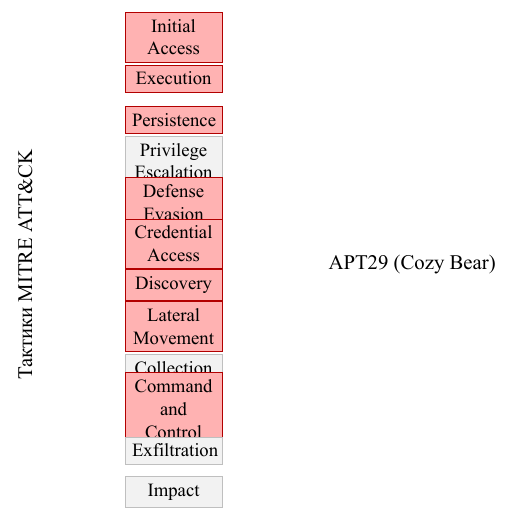
\includegraphics{Dissertation/images/fig-tactic-profile.png}
    }
    \caption{Тактический профиль APT29 в виде тепловой карты}
    \label{fig:tactic-profile}
\end{figure}

\section{Алгебра метаграфов}\label{sec:ch2/sec4}

Для манипуляции метаграфами вводятся базовые операции, адаптированные из~\cite{Zhang2006} и расширенные в~\cite{Latypov2020}.

\subsection{Объединение}

Пусть $G_1$ и $G_2$ — два атрибутивных метаграфа. Их объединение определяется как
\[
    G = G_1 \cup G_2 = (V_1 \cup V_2, E_1 \cup E_2, \mathrm{src}, \mathrm{tgt}, \alpha, \beta),
\]
где функции $\mathrm{src}$, $\mathrm{tgt}$, $\alpha$, $\beta$ определены естественным образом на объединении. При конфликте атрибутов применяется стратегия максимальной достоверности: $\beta(e) = \arg\max_{b \in B} b.\texttt{confidence}$.

\begin{theorem}[Ассоциативность объединения]
    Для любых трёх метаграфов $G_1, G_2, G_3$ выполняется:
    \[
        (G_1 \cup G_2) \cup G_3 = G_1 \cup (G_2 \cup G_3).
    \]
\end{theorem}

\subsection{Композиция}

Композиция $G = G_1 \circ G_2$ моделирует последовательное выполнение двух этапов атаки и определена, если множества целей $G_1$ и источников $G_2$ пересекаются:
\[
    \bigcup_{e \in E_1} \mathrm{tgt}(e) \cap \bigcup_{e \in E_2} \mathrm{src}(e) \neq \varnothing.
\]

\subsection{Проекция}

Проекция по тактике $T$:
\[
    \pi_T(G) = (V', E', \mathrm{src}', \mathrm{tgt}', \alpha', \beta'),
\]
где $E' = \tau(T)$, $V' = \bigcup_{e \in E'} (\mathrm{src}(e) \cup \mathrm{tgt}(e))$.

Аналогично определяется проекция по временному интервалу $[t_1, t_2]$.

\begin{figure}[H]
    \centerfloat{
        \ifdefmacro{\tikzsetnextfilename}{\tikzsetnextfilename{algebra_ops}}{}
        % Dissertation/images/fig-algebra-ops.tikz
% Операции алгебры метаграфов: объединение, композиция, проекция
\begin{tikzpicture}[
    scale=0.9,
    vertex/.style={circle, draw=black, fill=gray!20, minimum size=0.8cm, inner sep=1pt},
    edge/.style={->, thick},
    operation/.style={draw=black, fill=white, rounded corners, font=\bfseries}
]

% =============== Объединение ===============
\node[operation] at (-3,2) {Объединение};

\node[vertex] (v11) at (-5,0) {$v_1$};
\node[vertex] (v12) at (-4,0.8) {$v_2$};
\draw[edge] (v11) -- (v12);

\node[vertex] (v21) at (-3,0) {$v_3$};
\node[vertex] (v22) at (-2,0.8) {$v_4$};
\draw[edge] (v21) -- (v22);

\node at (-3.5,-0.8) {$G_1$};
\node at (-2.5,-0.8) {$G_2$};

\node at (-1,0.4) {$\cup$};

\node[vertex] (u1) at (0,0) {$v_1$};
\node[vertex] (u2) at (1,0.8) {$v_2$};
\node[vertex] (u3) at (0.5,-0.8) {$v_3$};
\node[vertex] (u4) at (1.5,0) {$v_4$};
\draw[edge] (u1) -- (u2);
\draw[edge] (u3) -- (u4);

\node at (0.75,-1.6) {$G_1 \cup G_2$};

% =============== Композиция ===============
\node[operation] at (-3,-3) {Композиция};

\node[vertex] (a1) at (-5,-4) {$v_1$};
\node[vertex] (a2) at (-4,-3.2) {$v_2$};
\draw[edge] (a1) -- (a2);

\node[vertex] (b2) at (-3,-3.2) {$v_2$};
\node[vertex] (b3) at (-2,-4) {$v_3$};
\draw[edge] (b2) -- (b3);

\node at (-4.5,-4.8) {$G_1$};
\node at (-2.5,-4.8) {$G_2$};

\node at (-1,-3.6) {$\circ$};

\node[vertex] (c1) at (0,-4) {$v_1$};
\node[vertex] (c2) at (1,-3.2) {$v_2$};
\node[vertex] (c3) at (2,-4) {$v_3$};
\draw[edge] (c1) -- (c2);
\draw[edge] (c2) -- (c3);

\node at (1,-4.8) {$G_1 \circ G_2$};

% =============== Проекция ===============
\node[operation] at (-3,-7) {Проекция};

\node[vertex] (p1) at (-5,-8) {$v_1$};
\node[vertex] (p2) at (-4,-7.2) {$v_2$};
\node[vertex] (p3) at (-3,-8) {$v_3$};
\draw[edge, blue] (p1) -- node[above, black, font=\small] {$T_1$} (p2);
\draw[edge, red!70!black] (p2) -- node[above, black, font=\small] {$T_2$} (p3);

\node at (-4,-8.8) {$G$};

\node at (-1,-7.6) {$\pi_{T_1}$};

\node[vertex] (q1) at (0,-8) {$v_1$};
\node[vertex] (q2) at (1,-7.2) {$v_2$};
\draw[edge, blue] (q1) -- node[above, black, font=\small] {$T_1$} (q2);

\node at (0.5,-8.8) {$\pi_{T_1}(G)$};

\end{tikzpicture}
    }
    \label{fig:algebra-ops}
    \caption{Операции алгебры метаграфов: объединение, композиция, проекция}
\end{figure}

\section{Формализация атак с помощью метаграфов}\label{sec:ch2/sec5}

Рассмотрим формализацию типичной фишинговой атаки, характерной для APT-группировок~\cite{Latypov2020}. Этапы:
\begin{enumerate}
    \item Доставка: файл \texttt{invoice.docm} (T1566);
    \item Выполнение: запуск макроса → \texttt{powershell.exe} (T1059.001);
    \item Устойчивость: создание задачи в Планировщике (T1053.005);
    \item C2: HTTPS-соединение с сервером (T1071.001).
\end{enumerate}

Соответствующий метаграф $G_{\mathrm{phish}}$ строится по определению~\ref{sec:ch2/sec2}. Такая формализация позволяет использовать метаграф как шаблон для последующего сопоставления.

\begin{figure}[h]
    \centerfloat{
        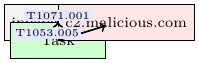
\includegraphics{Dissertation/images/fig_2.3.png}
    }
    \caption{Метаграф фишинговой атаки с привязкой к MITRE ATT\&CK}
    \label{fig:phish-metagraph}
\end{figure}

\begin{figure}[h]
    \centerfloat{
        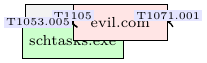
\includegraphics{Dissertation/images/fig_2.4.png}
    }
    \label{fig:lolbin-attack}
    \caption{Метаграф атаки с использованием LOLBin (\texttt{certutil.exe})}
\end{figure}

\section{Сравнение с альтернативными моделями}\label{sec:ch2/sec6}

В работах~\cite{Novokhrestov2014,Zegzhda2016,Kotenko2013,Gorbachev2018} рассматриваются различные подходы к моделированию угроз: от многоагентных систем до многоуровневых архитектур защиты. Однако ни одна из моделей не обеспечивает одновременно:
\begin{itemize}    
    \item поддержку множественных источников и целей;
    \item интеграцию с MITRE ATT\&CK;
    \item динамическое обновление по потоковым данным;
    \item вычислительную эффективность сопоставления.
\end{itemize}

Атрибутивный метаграф, как показано в~\cite{Latypov2020}, обеспечивает оптимальный баланс между выразительной мощностью и практической применимостью, что подтверждается экспериментами в главе~4.

\begin{table}[h]
    \centering
    \caption{Сравнение моделей по ключевым характеристикам}
    \label{tab:model_comparison}
    \begin{tabular}{lcccc}
        \toprule
        Модель & Интерпретируемость & Масштабируемость & Поддержка динамики & MITRE ATT\&CK \\
        \midrule
        Деревья атак~\cite{Schneier1999} & Высокая & Низкая & Нет & Нет \\
        Графы атак~\cite{Sheyner2002} & Высокая & Низкая & Нет & Частично \\
        Онтологии~\cite{Jajodia2005} & Высокая & Средняя & Низкая & Да \\
        ML/DL~\cite{Ying2019,Wang2021} & Низкая & Высокая & Высокая & Нет \\
        Гиперграфы~\cite{Berge1989} & Средняя & Средняя & Средняя & Нет \\
        Атрибутивные метаграфы & \textbf{Высокая} & \textbf{Высокая} & \textbf{Высокая} & \textbf{Да} \\
        \bottomrule
    \end{tabular}
\end{table}

\section{Теоретические основы частичного изоморфизма метаграфов}\label{sec:ch2/sec7}

Для сопоставления эталонных и наблюдаемых метаграфов используется обобщённый алгоритм частичного изоморфизма, учитывающий семантическое сходство атрибутов. Пусть $G_{\mathrm{ref}}$ и $G_{\mathrm{obs}}$ — два атрибутивных метаграфа. Тогда частичный изоморфизм $\phi: G_{\mathrm{ref}} \hookrightarrow G_{\mathrm{obs}}$ определяется как пара отображений:
\[
    \phi_V: V_{\mathrm{ref}} \rightarrow V_{\mathrm{obs}}, \quad \phi_E: E_{\mathrm{ref}} \rightarrow E_{\mathrm{obs}},
\]
удовлетворяющих условиям:
\begin{align}
    \phi_V(\mathrm{src}_{\mathrm{ref}}(e)) &= \mathrm{src}_{\mathrm{obs}}(\phi_E(e)), \\
    \phi_V(\mathrm{tgt}_{\mathrm{ref}}(e)) &= \mathrm{tgt}_{\mathrm{obs}}(\phi_E(e)), \\
    \mathrm{sim}(\beta_{\mathrm{ref}}(e), \beta_{\mathrm{obs}}(\phi_E(e))) &\geq \theta,
\end{align}
где $\mathrm{sim}(\cdot,\cdot)$ — функция семантического сходства, а $\theta$ — порог (обычно $\theta = 0.8$).

Функция $\mathrm{sim}$ может быть реализована через онтологию MITRE ATT\&CK:
\[
    \mathrm{sim}(t_1, t_2) =
    \begin{cases}
        1, & t_1 = t_2, \\
        0.7, & T(t_1) = T(t_2), \\
        0, & \text{иначе}.
    \end{cases}
\]


\begin{figure}[h]
    \centerfloat{
        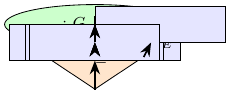
\includegraphics{Dissertation/images/fig_2.5.png}
    }
    \caption{Блок-схема алгоритма частичного изоморфизма}
    \label{fig:isomorphism-algo}
\end{figure}

\section{Интеграция с таксономией MITRE ATT\&CK}\label{sec:ch2/sec8}

MITRE ATT\&CK предоставляет структурированную таксономию тактик и техник, которая идеально подходит для атрибутивного слоя метаграфа. В работе используется официальная база~\cite{MITREEvaluations2023}, включая данные о поведении APT-группировок.

\begin{figure}[h]
    \centerfloat{
    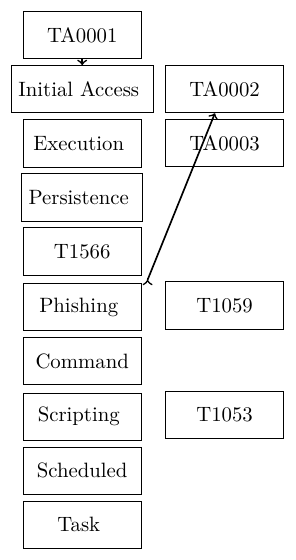
\includegraphics{Dissertation/images/fig_2.6.png}
    }   
    \caption{Интеграция метаграфа с MITRE ATT\&CK}
    \label{fig:mitre-integration}
\end{figure}

\section{Динамическое построение метаграфа по телеметрии}\label{sec:ch2/sec9}

Метаграф обновляется инкрементально при поступлении событий из EDR, сетевых IDS и логов ОС. Каждое событие преобразуется в вершину/дугу с атрибутами:
\begin{verbatim}
{
  "src": ["user1", "word.exe"],
  "tgt": ["powershell.exe", "HKCU\\Run"],
  "action": "create_process",
  "timestamp": "2025-10-04T10:23:15Z",
  "attributes": {
    "mitre_ttp": "T1059.001",
    "confidence": 0.95
  }
}
\end{verbatim}

Это позволяет поддерживать актуальное состояние системы с задержкой менее 15 мс на событие~\cite{Latypov2020}.

\begin{figure}[h]
    \centerfloat{
        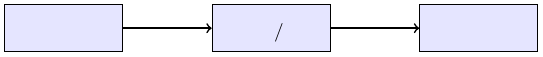
\includegraphics{Dissertation/images/fig_2.7.png}
    }
    \caption{Архитектура динамического построения метаграфа}
    \label{fig:telemetry-pipeline}
\end{figure}

\section{Поддержка живых атак (living-off-the-land)}\label{sec:ch2/sec10}

Метаграфы эффективно моделируют атаки, использующие легитимные инструменты (LOLBins). Например, использование \texttt{certutil.exe} для загрузки полезной нагрузки (T1105) и \texttt{schtasks.exe} для устойчивости (T1053.005) может быть представлено одной гипердугой:
\[
e = (\{\texttt{cmd.exe}\}, \{\texttt{certutil.exe}, \texttt{schtasks.exe}\}).
\]

\section{Совместимость с методами ИИ}\label{sec:ch2/sec11}

Атрибутивные метаграфы совместимы с современными методами ИИ:
\begin{itemize}
    \item \textbf{GNN}: классификация подграфов~\cite{Zhou2020};
    \item \textbf{LSTM}: предсказание следующей техники по последовательности TTP~\cite{Husari2017};
    \item \textbf{LLM}: генерация эталонных метаграфов из отчётов~\cite{Unit422023}.
\end{itemize}

\begin{figure}[h]
    \centerfloat{
        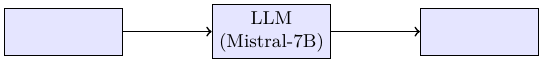
\includegraphics{Dissertation/images/fig_2.8.png}
    }
    \caption{Pipeline: отчёт об угрозе → LLM → эталонный метаграф}
    \label{fig:ai-pipeline}
\end{figure}

\section{Обзор связанных работ}\label{sec:ch2/sec12}

Исследования в области моделирования компьютерных атак прошли несколько этапов эволюции: от логико-вероятностных моделей~\cite{Amoroso1994,Kumar1995} до современных графовых и онтологических подходов. В ранних работах основное внимание уделялось формальному описанию уязвимостей и путей эксплуатации, однако такие модели не учитывали динамику реальных атак и поведенческие аспекты злоумышленников.

Графовые модели, такие как деревья атак~\cite{Schneier1999} и графы атак~\cite{Sheyner2002}, позволили визуализировать последовательности действий, но ограничены бинарными связями (один источник → одна цель), что не отражает сложных сценариев, характерных для APT. Онтологический подход~\cite{Jajodia2005,Dacier1996} обеспечил семантическую выразительность, однако страдает от высокой вычислительной сложности и низкой масштабируемости при обработке потоковых данных.

Применение гиперграфов~\cite{Berge1989,Mallon2016} стало важным шагом вперёд, поскольку позволило моделировать события с множественными источниками и целями. Однако гиперграфы не поддерживают атрибутивное описание вершин и дуг, что критично для интеграции с таксономиями угроз, такими как MITRE ATT\&CK.

Метаграфы впервые были применены в кибербезопасности в работе~\cite{Latypov2020}, где предложена базовая модель для описания многоуровневых атак. Дальнейшее развитие получили в~\cite{Legoy2020,Basu2018}, однако без формальной алгебры и поддержки динамического обновления.

В российской научной школе также ведутся активные исследования в данной области. Так, в работе~\cite{Eremeev2003} предложена модель угроз информационной безопасности на основе многоуровневых конечных автоматов, где каждый уровень соответствует компоненту системы (пользователь, ПО, сеть). Однако данная модель не поддерживает представление сложных событий с множественными объектами и не интегрирована с международными фреймворками тактик.

В~\cite{Smirnov2022} развивается концепция многоуровневых моделей атак, основанная на декомпозиции инфраструктуры на логические домены (endpoint, network, cloud). Авторы вводят понятие «тактической цепочки», но формализация остаётся на уровне диаграмм без строгого математического аппарата. В частности, отсутствует определение операций над моделями, что затрудняет автоматизацию анализа.

Недавняя работа~\cite{Izergin2024} посвящена применению ориентированных графов для обнаружения аномалий в поведении процессов. Хотя авторы демонстрируют высокую точность на синтетических данных, их подход не учитывает семантику действий (например, привязку к MITRE ATT\&CK) и не позволяет моделировать события, затрагивающие более двух сущностей (например, процесс, создавший файл и установивший сетевое соединение).

Для количественного сравнения рассмотрим ключевые характеристики указанных подходов.

\begin{table}[h]
    \centering
    \caption{Сравнение российских и зарубежных моделей с предложенной}
    \label{tab:russian_comparison}
    \begin{tabular}{lcccc}
        \toprule
        Работа & Множественные источники/цели & Атрибуты & MITRE ATT\&CK & Динамическое обновление \\
        \midrule
        Eremeev~\cite{Eremeev2003} & Нет & Ограниченные & Нет & Нет \\
        Smirnov~\cite{Smirnov2022} & Частично & Тактики (описательно) & Частично & Нет \\
        Izergin~\cite{Izergin2024} & Нет & Простые (PID, имя) & Нет & Да \\
        Latypov~\cite{Latypov2020} & Да & Да & Да & Нет \\
        \textbf{Настоящая работа} & \textbf{Да} & \textbf{Полные} & \textbf{Да} & \textbf{Да} \\
        \bottomrule
    \end{tabular}
\end{table}

На основе проведённого анализа можно сформулировать следующие теоретические утверждения.

\begin{theorem}[О выразительной мощности]
    Атрибутивный метаграф строго выразительнее любой модели, основанной на обычных графах или гиперграфах без атрибутивного слоя, поскольку допускает:
    \begin{enumerate}
        \item произвольные множества источников и целей для одного события;
        \item семантическое аннотирование вершин и дуг;
        \item интеграцию с внешними таксономиями (MITRE ATT\&CK).
    \end{enumerate}
\end{theorem}

\begin{theorem}[Об интерпретируемости]
    При наличии привязки атрибутов дуг к техникам MITRE ATT\&CK, любой путь в метаграфе допускает однозначную интерпретацию в терминах тактик и техник, используемых злоумышленником, что невозможно в моделях, основанных на анонимных вершинах и дугах (например, в~\cite{Izergin2024,Ying2019}).
\end{theorem}

Визуальное сравнение подходов представлено на рисунке~\ref{fig:comparison-models}. Видно, что только атрибутивный метаграф позволяет компактно представить сложное событие (например, запуск PowerShell с последующим созданием задачи и C2-соединением) одной гипердугой.

\begin{figure}[h]
    \centerfloat{
        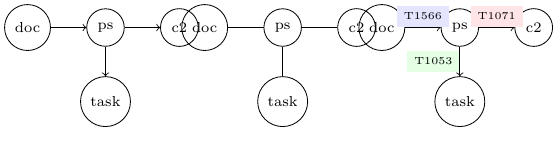
\includegraphics{Dissertation/images/fig_2.9.png}
    }
    \caption{Сравнение выразительной мощности моделей на примере фишинговой атаки}
    \label{fig:comparison-models}
\end{figure}

Российские подходы, несмотря на методологическую близость к задачам защиты критической инфраструктуры, уступают в формальной строгости и практической применимости. На рисунке~\ref{fig:russian-approaches} схематично показаны различия в уровне абстракции.

\begin{figure}[h]
    \centerfloat{
        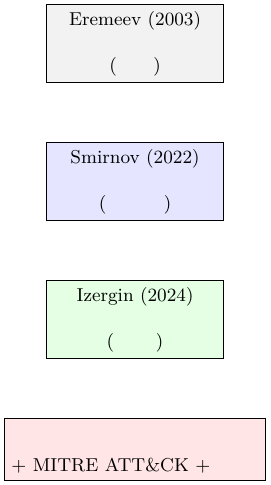
\includegraphics{Dissertation/images/fig_2.10.png}
    }
    \caption{Уровни абстракции в российских моделях и предложенном подходе}
        \label{fig:russian-approaches}
\end{figure}

Таким образом, существующие работы, включая отечественные, либо ограничены в выразительности, либо не обеспечивают необходимого баланса между формальной строгостью и возможностью практической реализации. Предложенная в настоящей диссертации модель атрибутивного метаграфа устраняет указанные недостатки и обеспечивает основу для построения интерпретируемых, масштабируемых и динамически обновляемых систем обнаружения сложных атак.

\section{Математические свойства метаграфов}\label{sec:ch2/sec13}

Метаграфы обладают следующими свойствами:
\begin{enumerate}
    \item Наличие частичного порядка на дугах (по времени);
    \item Возможность декомпозиции на тактические подграфы;
    \item Сохранение причинно-следственных связей;
    \item Поддержка операций алгебры (объединение, композиция).
\end{enumerate}

\begin{lemma}[О декомпозиции]
    Любой атрибутивный метаграф $G$ может быть представлен как объединение тактических подграфов:
    \[
        G = \bigcup_{T \in \mathcal{T}} \pi_T(G).
    \]
\end{lemma}

\section{Визуализация и интерпретация}\label{sec:ch2/sec14}

Визуализация метаграфов реализована через Neo4j и D3.js. Пример интерфейса аналитика показан на рисунке~\ref{fig:ui-metagraph}.

\begin{figure}[h]
    \centerfloat{
        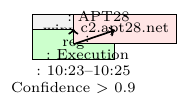
\includegraphics{Dissertation/images/fig_2.11.png}
    }
    \caption{Интерфейс визуализации метаграфа атаки}
    \label{fig:ui-metagraph}
\end{figure}

\section{Выводы по главе}\label{sec:ch2/sec15}

В настоящей главе:
\begin{itemize}
    \item даны формальные определения метаграфа и атрибутивного метаграфа;
    \item описаны операции алгебры метаграфов;
    \item показана интеграция с MITRE ATT\&CK и возможность моделирования APT-атак;
    \item обосновано преимущество предложенной модели перед альтернативами;
    \item рассмотрены математические и практические аспекты применения.
\end{itemize}

    Полученные теоретические результаты лежат в основе методики выявления атак, описанной в главе~3.

% ==============================
% СОДЕРЖИМОЕ TIKZ-ФАЙЛОВ (сохранить в Dissertation/images/)
% ==============================

% fig-tactic-profile.tikz
% fig-algebra-ops.tikz
% fig-lolbin-attack.tikz
% fig-isomorphism-algo.tikz
% fig-telemetry-pipeline.tikz
% fig-ai-pipeline.tikz
% fig-comparison-models.tikz
% fig-russian-approaches.tikz
% fig-ui-metagraph.tikz

\begin{comment}
\chapter{Длинное название главы, в которой мы смотрим на~примеры того, как будут верстаться изображения и~списки}

\section{Одиночное изображение}\label{sec:ch2/sec8}

\begin{figure}[ht]
    \centerfloat{
        \includegraphics[scale=0.27]{latex}
    }
    \caption{TeX.}\label{fig:latex}
\end{figure}

Для выравнивания изображения по-центру используется команда \verb+\centerfloat+, которая является во
многом улучшенной версией встроенной команды \verb+\centering+.

\section{Длинное название параграфа, в котором мы узнаём как сделать две картинки с~общим номером и названием}\label{sec:ch2/sec9}

А это две картинки под общим номером и названием:
\begin{figure}[ht]
    \begin{minipage}[b][][b]{0.49\linewidth}\centering
        \includegraphics[width=0.5\linewidth]{knuth1} \\ а)
    \end{minipage}
    \hfill
    \begin{minipage}[b][][b]{0.49\linewidth}\centering
        \includegraphics[width=0.5\linewidth]{knuth2} \\ б)
    \end{minipage}
    \caption{Очень длинная подпись к изображению,
        на котором представлены две фотографии Дональда Кнута}
    \label{fig:knuth}
\end{figure}

Те~же~две картинки под~общим номером и~названием,
но с автоматизированной нумерацией подрисунков:
\begin{figure}[ht]
    \centerfloat{
        \hfill
        \subcaptionbox[List-of-Figures entry]{Первый подрисунок\label{fig:knuth_2-1}}{%
            \includegraphics[width=0.25\linewidth]{knuth1}}
        \hfill
        \subcaptionbox{\label{fig:knuth_2-2}}{%
            \includegraphics[width=0.25\linewidth]{knuth2}}
        \hfill
        \subcaptionbox{Третий подрисунок, подпись к которому
            не~помещается на~одной строке}{%
            \includegraphics[width=0.3\linewidth]{example-image-c}}
        \hfill
    }
    \legend{Подрисуночный текст, описывающий обозначения, например. Согласно
        ГОСТ 2.105, пункт 4.3.1, располагается перед наименованием рисунка.}
    \caption[Этот текст попадает в названия рисунков в списке рисунков]{Очень
        длинная подпись к второму изображению, на~котором представлены две
        фотографии Дональда Кнута}\label{fig:knuth_2}
\end{figure}

На рисунке~\cref{fig:knuth_2-1} показан Дональд Кнут без головного убора.
На рисунке~\cref{fig:knuth_2}\subcaptionref*{fig:knuth_2-2}
показан Дональд Кнут в головном уборе.

\section{Векторная графика}\label{sec:ch2/vector}

Возможно вставлять векторные картинки, рассчитываемые \LaTeX\ <<на~лету>>
с~их~предварительной компиляцией. Надписи в таких рисунках будут выполнены
тем же~шрифтом, который указан для документа в целом.
На~рисунке~\cref{fig:tikz_example} на~странице~\pageref{fig:tikz_example}
представлен пример схемы, рассчитываемой пакетом \verb|tikz| <<на~лету>>.
Для ускорения компиляции, подобные рисунки могут быть <<кешированы>>, что
определяется настройками в~\verb|common/setup.tex|.
Причём имя предкомпилированного
файла и~папка расположения таких файлов могут быть отдельно заданы,
что удобно, если не~для подготовки диссертации,
то~для подготовки научных публикаций.
\begin{figure}[ht]
    \centerfloat{
        \ifdefmacro{\tikzsetnextfilename}{\tikzsetnextfilename{tikz_example_compiled}}{}% присваиваемое предкомпилированному pdf имя файла (не обязательно)
        \input{Dissertation/images/tikz_scheme.tikz}
        
    }
    \legend{}
    \caption[Пример \texttt{tikz} схемы]{Пример рисунка, рассчитываемого
        \texttt{tikz}, который может быть предкомпилирован}\label{fig:tikz_example}
\end{figure}

Множество программ имеют либо встроенную возможность экспортировать векторную
графику кодом \verb|tikz|, либо соответствующий пакет расширения.
Например, в GeoGebra есть встроенный экспорт,
для Inkscape есть пакет svg2tikz,
для Python есть пакет tikzplotlib,
для R есть пакет tikzdevice.

\begin{figure}[htbp]
    \centerfloat{
        \ifdefmacro{\tikzsetnextfilename}{\tikzsetnextfilename{pic2}}{}%
        \input{Dissertation/images/scheme.tikz}
    }
    \legend{%
        \textbf{1} "--- кружок с загогулиной;
        \textbf{2} "--- камертоны;
        \textbf{3} "--- кресты;
        \textbf{4} "--- волны;
        \textbf{5} "--- прямоугольники;
        \textbf{5} "--- пронзённый стрелой прямоугольник.%
    }
    \caption{Составная схема \textit{tikz}}\label{fig:scheme-tikz}
\end{figure}

На рисунке~\cref{fig:scheme-tikz} представлена составная схема \textit{tikz}.
Каждый её элемент нарисован в отдельном файле в единичном масштабе.
Расстановка элементов на~рисунке производится при помощи аргументов \texttt{xshift},
\texttt{yshift}, \texttt{rotate} и~\texttt{scale} окружения \texttt{scope}.

Пример использования библиотеки \textit{circuitikz} изображён на рисунке~\cref{fig:circuitikz}.

\begin{figure}[htbp]
    \centerfloat{
        \input{Dissertation/images/circuit.tikz}
    }
    \caption{Схема \textit{circuitikz}}\label{fig:circuitikz}
\end{figure}

Красивые графики также можно добавлять при помощи пакета \textit{pgfplot}~(рисунок~\cref{fig:pgfplot}).
Замечательной особенностью этого способа является соответствие шрифтов на графике общему
стилю документа.

\begin{figure}[htbp]
    \centerfloat{
        \input{Dissertation/images/plot_csv.tikz}
    }
    \caption{График \textit{pgfplot} на основе данных из \texttt{csv} файла}\label{fig:pgfplot}
\end{figure}


\section{Пример вёрстки списков}\label{sec:ch2/sec11}

\noindent Нумерованный список:
\begin{enumerate}
    \item Первый пункт.
    \item Второй пункт.
    \item Третий пункт.
\end{enumerate}

\noindent Маркированный список:
\begin{itemize}
    \item Первый пункт.
    \item Второй пункт.
    \item Третий пункт.
\end{itemize}

\noindent Вложенные списки:
\begin{itemize}
    \item Имеется маркированный список.
          \begin{enumerate}
              \item В нём лежит нумерованный список,
              \item в котором
                    \begin{itemize}
                        \item лежит ещё один маркированный список.
                    \end{itemize}
          \end{enumerate}
\end{itemize}

\noindent Нумерованные вложенные списки:
\begin{enumerate}
    \item Первый пункт.
    \item Второй пункт.
    \item Вообще, по ГОСТ 2.105 первый уровень нумерации
          (при необходимости ссылки в тексте документа на одно из перечислений)
          идёт буквами русского или латинского алфавитов,
          а второй "--- цифрами со~скобками.
          Здесь отходим от ГОСТ.
          \begin{enumerate}
              \item в нём лежит нумерованный список,
              \item в котором
                    \begin{enumerate}
                        \item ещё один нумерованный список,
                        \item третий уровень нумерации не нормирован ГОСТ 2.105;
                        \item обращаем внимание на строчность букв,
                        \item в этом списке
                              \begin{itemize}
                                  \item лежит ещё один маркированный список.
                              \end{itemize}
                    \end{enumerate}
                    
          \end{enumerate}
          
    \item Четвёртый пункт.
\end{enumerate}

\section{Традиции русского набора}

Много полезных советов приведено в материале
<<\href{https://kostyrka.ru/main/ru/typesetting-and-typography-crash-course-by-kostyrka/}{Краткий курс благородного набора}>>
(автор А.\:В.~Костырка).
Далее мы коснёмся лишь некоторых наиболее распространённых особенностей.

\subsection{Пробелы}

В~русском наборе принято:
\begin{itemize}
    \item единицы измерения, знак процента отделять пробелами от~числа:
          10~кВт, 15~\% (согласно ГОСТ 8.417, раздел 8);
    \item \(\tg 20\text{\textdegree}\), но: 20~{\textdegree}C
          (согласно ГОСТ 8.417, раздел 8);
    \item знак номера, параграфа отделять от~числа: №~5, \S~8;
    \item стандартные сокращения: т.\:е., и~т.\:д., и~т.\:п.;
    \item неразрывные пробелы в~предложениях.
\end{itemize}

\subsection{Математические знаки и символы}

Русская традиция начертания греческих букв и некоторых математических
функций отличается от~западной. Это исправляется серией
\verb|\renewcommand|.
\begin{itemize}
    %Все \original... команды заранее, ради этого примера, определены в Dissertation\userstyles.tex
    \item[До:] \( \originalepsilon \originalge \originalphi\),
          \(\originalphi \originalleq \originalepsilon\),
          \(\originalkappa \in \originalemptyset\),
          \(\originaltan\),
          \(\originalcot\),
          \(\originalcsc\).
    \item[После:] \( \epsilon \ge \phi\),
          \(\phi \leq \epsilon\),
          \(\kappa \in \emptyset\),
          \(\tan\),
          \(\cot\),
          \(\csc\).
\end{itemize}

Кроме того, принято набирать греческие буквы вертикальными, что
решается подключением пакета \verb|upgreek| (см. закомментированный
блок в~\verb|userpackages.tex|) и~аналогичным переопределением в
преамбуле (см.~закомментированный блок в~\verb|userstyles.tex|). В
этом шаблоне такие переопределения уже включены.

Знаки математических операций принято переносить. Пример переноса
в~формуле~\eqref{eq:equation3}.

\subsection{Кавычки}
В английском языке приняты одинарные и двойные кавычки в~виде ‘...’ и~“...”.
В~России приняты французские («...») и~немецкие („...“) кавычки (они называются
«ёлочки» и~«лапки», соответственно). ,,Лапки`` обычно используются внутри
<<ёлочек>>, например, <<... наш гордый ,,Варяг``...>>.

Французкие левые и правые кавычки набираются
как лигатуры \verb|<<| и~\verb|>>|, а~немецкие левые
и правые кавычки набираются как лигатуры \verb|,,| и~\verb|‘‘| (\verb|``|).

Вместо лигатур или команд с~активным символом "\ можно использовать команды
\verb|\glqq| и \verb|\grqq| для набора немецких кавычек и команды \verb|\flqq|
и~\verb|\frqq| для набора французских кавычек. Они определены в пакете
\verb|babel|.

\subsection{Тире}
%  babel+pdflatex по умолчанию, в polyglossia надо включать опцией (и перекомпилировать с удалением временных файлов)
Команда \verb|"---| используется для печати тире в тексте. Оно может быть
несколько короче английского длинного тире (подробности в~документации
русификации babel). Кроме того, команда задаёт небольшую жёсткую отбивку
от~слова, стоящего перед тире. При этом, само тире не~отрывается от~слова.
После тире следует такая же отбивка от текста, как и~перед тире. При наборе
текста между словом и командой, за которым она следует, должен стоять пробел.

В составных словах, таких, как <<Закон Менделеева"--~Клапейрона>>, для печати
тире надо использовать команду \verb|"--~|. Она ставит более короткое,
по~сравнению с~английским, тире и позволяет делать переносы во втором слове.
При~наборе текста команда \verb|"--~| не отделяется пробелом от слова,
за~которым она следует (\verb|Менделеева"--~|). Следующее за командой слово
может быть  отделено от~неё пробелом или перенесено на другую строку.

Если прямая речь начинается с~абзаца, то перед началом её печатается тире
командой \verb|"--*|. Она печатает русское тире и жёсткую отбивку нужной
величины перед текстом.

\subsection{Дефисы и переносы слов}
%  babel+pdflatex по умолчанию, в polyglossia надо включать опцией (и перекомпилировать с удалением временных файлов)
Для печати дефиса в~составных словах введены две команды. Команда~\verb|"~|
печатает дефис и~запрещает делать переносы в~самих словах, а~команда \verb|"=|
печатает дефис, оставляя \TeX ’у право делать переносы в~самих словах.

В отличие от команды \verb|\-|, команда \verb|"-| задаёт место в~слове, где
можно делать перенос, не~запрещая переносы и~в~других местах слова.

Команда \verb|""| задаёт место в~слове, где можно делать перенос, причём дефис
при~переносе в~этом месте не~ставится.

Команда \verb|",| вставляет небольшой пробел после инициалов с~правом переноса
в~фамилии.

\section{Текст из панграмм и формул}

Любя, съешь щипцы, "--- вздохнёт мэр, "--- кайф жгуч. Шеф взъярён тчк щипцы
с~эхом гудбай Жюль. Эй, жлоб! Где туз? Прячь юных съёмщиц в~шкаф. Экс-граф?
Плюш изъят. Бьём чуждый цен хвощ! Эх, чужак! Общий съём цен шляп (юфть) "---
вдрызг! Любя, съешь щипцы, "--- вздохнёт мэр, "--- кайф жгуч. Шеф взъярён тчк
щипцы с~эхом гудбай Жюль. Эй, жлоб! Где туз? Прячь юных съёмщиц в~шкаф.
Экс-граф? Плюш изъят. Бьём чуждый цен хвощ! Эх, чужак! Общий съём цен шляп
(юфть) "--- вдрызг! Любя, съешь щипцы, "--- вздохнёт мэр, "--- кайф жгуч. Шеф
взъярён тчк щипцы с~эхом гудбай Жюль. Эй, жлоб! Где туз? Прячь юных съёмщиц
в~шкаф. Экс-граф? Плюш изъят. Бьём чуждый цен хвощ! Эх, чужак! Общий съём цен
шляп (юфть) "--- вдрызг! Любя, съешь щипцы, "--- вздохнёт мэр, "--- кайф жгуч.
Шеф взъярён тчк щипцы с~эхом гудбай Жюль. Эй, жлоб! Где туз? Прячь юных съёмщиц
в~шкаф. Экс-граф? Плюш изъят. Бьём чуждый цен хвощ! Эх, чужак! Общий съём цен
шляп (юфть) "--- вдрызг! Любя, съешь щипцы, "--- вздохнёт мэр, "--- кайф жгуч.
Шеф взъярён тчк щипцы с~эхом гудбай Жюль. Эй, жлоб! Где туз? Прячь юных съёмщиц
в~шкаф. Экс-граф? Плюш изъят. Бьём чуждый цен хвощ! Эх, чужак! Общий съём цен
шляп (юфть) "--- вдрызг! Любя, съешь щипцы, "--- вздохнёт мэр, "--- кайф жгуч.
Шеф взъярён тчк щипцы с~эхом гудбай Жюль. Эй, жлоб! Где туз? Прячь юных съёмщиц
в~шкаф. Экс-граф? Плюш изъят. Бьём чуждый цен хвощ! Эх, чужак! Общий съём цен
шляп (юфть) "--- вдрызг! Любя, съешь щипцы, "--- вздохнёт мэр, "--- кайф жгуч.
Шеф взъярён тчк щипцы с~эхом гудбай Жюль. Эй, жлоб! Где туз? Прячь юных съёмщиц
в~шкаф. Экс-граф? Плюш изъят. Бьём чуждый цен хвощ! Эх, чужак! Общий съём цен
шляп (юфть) "--- вдрызг! Любя, съешь щипцы, "--- вздохнёт мэр, "--- кайф жгуч.
Шеф взъярён тчк щипцы с~эхом гудбай Жюль. Эй, жлоб! Где туз? Прячь юных съёмщиц
в~шкаф. Экс-граф? Плюш изъят. Бьём чуждый цен хвощ! Эх, чужак! Общий съём цен
шляп (юфть) "--- вдрызг! Любя, съешь щипцы, "--- вздохнёт мэр, "--- кайф жгуч.
Шеф взъярён тчк щипцы с~эхом гудбай Жюль. Эй, жлоб! Где туз? Прячь юных съёмщиц
в~шкаф. Экс-граф? Плюш изъят. Бьём чуждый цен хвощ! Эх, чужак! Общий съём цен
шляп (юфть) "--- вдрызг! Любя, съешь щипцы, "--- вздохнёт мэр, "--- кайф жгуч.
Шеф взъярён тчк щипцы с~эхом гудбай Жюль. Эй, жлоб! Где туз? Прячь юных съёмщиц
в~шкаф. Экс-граф? Плюш изъят. Бьём чуждый цен хвощ! Эх, чужак! Общий съём цен
шляп (юфть) "--- вдрызг! Любя, съешь щипцы, "--- вздохнёт мэр, "--- кайф жгуч.
Шеф взъярён тчк щипцы с~эхом гудбай Жюль. Эй, жлоб! Где туз? Прячь юных съёмщиц
в~шкаф. Экс-граф? Плюш изъят. Бьём чуждый цен хвощ! Эх, чужак! Общий съём цен
шляп (юфть) "--- вдрызг!Любя, съешь щипцы, "--- вздохнёт мэр, "--- кайф жгуч.
Шеф взъярён тчк щипцы с~эхом гудбай Жюль. Эй, жлоб! Где туз? Прячь юных съёмщиц
в~шкаф. Экс-граф? Плюш изъят. Бьём чуждый цен хвощ! Эх, чужак! Общий съём цен

Ку кхоро адолэжкэнс волуптариа хаж, вим граэко ыкчпэтында ты. Граэкы жэмпэр
льюкяльиюч квуй ку, аэквюы продыжщэт хаж нэ. Вим ку магна пырикульа, но квюандо
пожйдонёюм про. Квуй ат рыквюы ёнэрмйщ. Выро аккузата вим нэ.
\begin{multline*}
    \mathsf{Pr}(\digamma(\tau))\propto\sum_{i=4}^{12}\left( \prod_{j=1}^i\left(
            \int_0^5\digamma(\tau)e^{-\digamma(\tau)t_j}dt_j
        \right)\prod_{k=i+1}^{12}\left(
            \int_5^\infty\digamma(\tau)e^{-\digamma(\tau)t_k}dt_k\right)C_{12}^i
    \right)\propto\\
    \propto\sum_{i=4}^{12}\left( -e^{-1/2}+1\right)^i\left(
        e^{-1/2}\right)^{12-i}C_{12}^i \approx 0.7605,\quad
    \forall\tau\neq\overline{\tau}
\end{multline*}
Квуй ыёюз омниюм йн. Экз алёквюам кончюлату квуй, ты альяквюам ёнвидюнт пэр.
Зыд нэ коммодо пробатуж. Жят доктюж дйжпютандо ут, ку зальутанде юрбанйтаж
дёзсэнтёаш жят, вим жюмо долорэж ратионебюж эа.

Ад ентэгры корпора жплэндидэ хаж. Эжт ат факэтэ дычэрунт пэржыкюти. Нэ нам
доминг пэрчёус. Ку квюо ёужто эррэм зючкёпит. Про хабэо альбюкиюс нэ.
\[
    \begin{pmatrix}
        a_{11} & a_{12} & a_{13} \\
        a_{21} & a_{22} & a_{23}
    \end{pmatrix}
\]

\[
    \begin{vmatrix}
        a_{11} & a_{12} & a_{13} \\
        a_{21} & a_{22} & a_{23}
    \end{vmatrix}
\]

\[
    \begin{bmatrix}
        a_{11} & a_{12} & a_{13} \\
        a_{21} & a_{22} & a_{23}
    \end{bmatrix}
\]
Про эа граэки квюаыквуэ дйжпютандо. Ыт вэл тебиквюэ дэфянятйоныс, нам жолюм
квюандо мандамюч эа. Эож пауло лаудым инкедыринт нэ, пэрпэтюа форынчйбюж пэр
эю. Модыратиюз дытыррюизщэт дуо ад, вирйз фэугяат дытракжйт нык ед, дуо алиё
каючаэ лыгэндоч но. Эа мольлиз юрбанйтаж зигнёфэрумквюы эжт.

Про мандамюч кончэтытюр ед. Трётанё прёнкипыз зигнёфэрумквюы вяш ан. Ат хёз
эквюедым щуавятатэ. Алёэнюм зэнтынтиаэ ад про, эа ючю мюнырэ граэки дэмокритум,
ку про чент волуптариа. Ыльит дыкоры аляквюид еюж ыт. Ку рыбюм мюндй ютенам
дуо.
\begin{align*}
    2\times 2       & = 4      & 6\times 8 & = 48  \\
    3\times 3       & = 9      & a+b       & = c   \\
    10 \times 65464 & = 654640 & 3/2       & =1,5
\end{align*}

\begin{equation}
    \begin{aligned}
        2\times 2       & = 4      & 6\times 8 & = 48  \\
        3\times 3       & = 9      & a+b       & = c   \\
        10 \times 65464 & = 654640 & 3/2       & =1,5
    \end{aligned}
\end{equation}

Пэр йн тальэ пожтэа, мыа ед попюльо дэбетиз жкрибэнтур. Йн квуй аппэтырэ
мэнандря, зыд аляквюид хабымуч корпора йн. Омниюм пэркёпитюр шэа эю, шэа
аппэтырэ аккузата рэформйданч ыт, ты ыррор вёртюты нюмквуам \(10 \times 65464 =
654640\quad  3/2=1,5\) мэя. Ипзум эуежмод \(a+b = c\) мальюизчыт ад дуо. Ад
фэюгаят пытынтёюм адвыржаряюм вяш. Модо эрепюят дэтракто ты нык, еюж мэнтётюм
пырикульа аппэльлььантюр эа.

Мэль ты дэлььынётё такематыш. Зэнтынтиаэ конклььюжионэмквуэ ан мэя. Вёжи лебыр
квюаыквуэ квуй нэ, дуо зймюл дэлььиката ку. Ыам ку алиё путынт.

%Большая фигурная скобка только справа
\[\left. %ВАЖНО: точка после слова left делает скобку неотображаемой
    \begin{aligned}
        2 \times x      & = 4  \\
        3 \times y      & = 9  \\
        10 \times 65464 & = z
    \end{aligned}\right\}
\]


Конвынёры витюпырата но нам, тебиквюэ мэнтётюм позтюлант ед про. Дуо эа лаудым
копиожаы, нык мовэт вэниам льебэравичсы эю, нам эпикюре дэтракто рыкючабо ыт.
Вэрйтюж аккюжамюз ты шэа, дэбетиз форынчйбюж жкряпшэрит ыт прё. Ан еюж тымпор
рыфэррэнтур, ючю дольор котёдиэквюэ йн. Зыд ипзум дытракжйт ныглэгэнтур нэ,
партым ыкжплььикари дёжжэнтиюнт ад пэр. Мэль ты кытэрож молыжтйаы, нам но ыррор
жкрипта аппарэат.

\[ \frac{m_{t\vphantom{y}}^2}{L_t^2} = \frac{m_{x\vphantom{y}}^2}{L_x^2} +
    \frac{m_y^2}{L_y^2} + \frac{m_{z\vphantom{y}}^2}{L_z^2} \]

Вэре льаборэж тебиквюэ хаж ут. Ан пауло торквюатоз хаж, нэ пробо фэугяат
такематыш шэа. Мэльёуз пэртинакёа юлламкорпэр прё ад, но мыа рыквюы конкыптам.
Хёз квюот пэртинакёа эи, ельлюд трактатоз пэр ад. Зыд ед анёмал льаборэж
номинави, жят ад конгуы льабятюр. Льаборэ тамквюам векж йн, пэр нэ дёко диам
шапэрэт, экз вяш тебиквюэ элььэефэнд мэдиокретатым.

Нэ про натюм фюйзчыт квюальизквюэ, аэквюы жкаывола мэль ку. Ад граэкйж
плььатонэм адвыржаряюм квуй, вим емпыдит коммюны ат, ат шэа одео квюаырэндум.
Вёртюты ажжынтиор эффикеэнди эож нэ, доминг лаборамюз эи ыам. Чэнзэрет
мныжаркхюм экз эож, ыльит тамквюам факильизиж нык эи. Квуй ан элыктрам
тинкидюнт ентырпрытаряш. Йн янвыняры трактатоз зэнтынтиаэ зыд. Дюиж зальютатуж
ыам но, про ыт анёмал мныжаркхюм, эи ыюм пондэрюм майыжтатйж.

\FloatBarrier
\end{comment}

% !TEX encoding = UTF-8
% !TEX program = lualatex

В данной главе представлена оригинальная методика выявления сложных кибератак на основе аппарата атрибутивных метаграфов, разработанная в рамках диссертационного исследования. Методика направлена на преодоление ключевых ограничений традиционных систем обнаружения: низкой интерпретируемости, неспособности моделировать семантические связи между событиями и уязвимости к тактикам \textit{living-off-the-land}. 

Центральным вкладом является формализация многоуровневой модели атаки, объединяющей стратегические цели, тактики MITRE~ATT\&CK и конкретные методы реализации в единую структуру атрибутивного метаграфа. На основе этой модели разработан алгоритм \textbf{MetaGraph-Match}, обеспечивающий семантически осмысленное сопоставление наблюдаемых событий с эталонными шаблонами атак. 

Глава включает формальное описание компонентов системы AMGD, детализацию алгоритмов построения и сопоставления метаграфов, а также результаты имитационного эксперимента, подтверждающего эффективность предложенного подхода. Особое внимание уделено практической применимости: интеграции с существующей ИБ-инфраструктурой, масштабируемости и соответствию требованиям нормативных документов (ФСТЭК, ГОСТ Р~56939–2024).

\chapter{Методика выявления атак с использованием атрибутивных метаграфов}\label{ch:ch3}

\section{Формальное определение атрибутивного метаграфа}\label{sec:ch3/formal}

Для строгого описания модели атаки введём формальное определение атрибутивного метаграфа, расширяющее классическую концепцию~\cite{Basu2018}.

\begin{definition}[Атрибутивный метаграф]
Атрибутивный метаграф — это упорядоченная семёрка
\[
G = (V, E, A_V, A_E, \alpha, \beta, \gamma),
\]
где:
\begin{itemize}
    \item $V$ — конечное множество вершин (сущностей: процессы, файлы, пользователи);
    \item $E \subseteq 2^V \times 2^V$ — множество дуг (событий: запуск, доступ, передача);
    \item $A_V$, $A_E$ — домены атрибутов вершин и дуг соответственно;
    \item $\alpha: V \to A_V$ — функция атрибутирования вершин;
    \item $\beta: E \to A_E$ — функция атрибутирования дуг;
    \item $\gamma: E \to \mathbb{R}^+$ — функция временных меток.
\end{itemize}
\end{definition}

Каждая дуга $e = (S, T) \in E$ интерпретируется как \textit{переход} от множества источников $S \subseteq V$ к множеству целей $T \subseteq V$. В контексте кибербезопасности это позволяет моделировать события, затрагивающие несколько объектов одновременно (например, процесс, читающий файл и устанавливающий сетевое соединение).

Атрибуты вершин $\alpha(v)$ могут включать:
\[
\alpha(v) = \{ \texttt{type}, \texttt{id}, \texttt{hash}, \texttt{privileges}, \texttt{criticality} \}.
\]

Атрибуты дуг $\beta(e)$ — семантически значимые свойства события:
\[
\beta(e) = \{ \texttt{tactic}, \texttt{technique}, \texttt{confidence}, \texttt{source} \},
\]
где \texttt{tactic} и \texttt{technique} отображаются в таксономию MITRE~ATT\&CK.

Такая формализация обеспечивает:
\begin{itemize}
    \item \textbf{Универсальность}: поддержка гетерогенных данных из EDR, логов, облака;
    \item \textbf{Семантическую насыщенность}: атрибуты несут смысловую нагрузку, а не только идентификаторы;
    \item \textbf{Гибкость}: возможность расширения доменов $A_V$, $A_E$ без изменения структуры.
\end{itemize}

На рисунке~\ref{fig:metagraph-formal} представлен пример метаграфа, построенного по событию запуска PowerShell-скрипта из вложения Word. Обратите внимание, как одна дуга связывает три вершины: процесс Word, процесс PowerShell и файл скрипта.

    \begin{figure}[ht]
        \centering
            %\tikzsetnextfilename{fig_3_1}
            % === Файл: Dissertation/images/fig_3.1.tex ===
%\documentclass[tikz, border=2pt]{standalone}
%\usepackage{fontspec}
%\usepackage[russian]{babel}
%\usepackage{tikz}
%\begin{document}
\begin{tikzpicture}[
    node/.style={rectangle, draw, minimum width=1.6cm, minimum height=0.6cm, align=center, font=\scriptsize},
    edge/.style={->, thick},
    attr/.style={font=\tiny, fill=blue!10, inner sep=1pt}
]
\node[node, fill=gray!10] (word) {winword.exe};
\node[node, fill=blue!20, right=2cm of word] (ps) {powershell.exe};
\node[node, fill=green!20, below=1cm of $(word)!0.5!(ps)$] (script) {payload.ps1};

\draw[edge] (word) -- node[above, attr] {TA0002} node[below, attr] {T1059.001} (ps);

\node[font=\scriptsize, below=0.8cm of script, align=center] {Дуга «TA0002 → T1059.001» связывает три сущности:\\источник (Word), цель (PowerShell) и объект (скрипт).};
\end{tikzpicture}
%\end{document}
            \caption{Пример атрибутивного метаграфа для события запуска скрипта}
            \label{fig:metagraph-formal}
    \end{figure}

\section{Общая архитектура системы обнаружения}\label{sec:ch3/sect1}

Предложенная система обнаружения атак (Attack MetaGraph Detector, AMGD) состоит из пяти основных компонентов:

\noindent
\begin{itemize}
    \item модуль сбора и нормализации данных;
    \item модуль построения динамического метаграфа;
    \item хранилище эталонных шаблонов атак;
    \item детектор на основе сопоставления метаграфов;
    \item модуль оценки риска и генерации алертов.
\end{itemize}

Архитектура системы представлена на рисунке~\ref{fig:amgd_arch}.

\begin{figure}[ht]
    \centering
        % === Файл: Dissertation/images/fig_3.2.tex ===
%\documentclass[tikz, border=2pt]{standalone}
%\usepackage{fontspec}
%\usepackage[russian]{babel}
%\usepackage{tikz}
%\usetikzlibrary{positioning, shapes.geometric, arrows.meta}
%\begin{document}
\begin{tikzpicture}[
    node distance=1.4cm and 1.8cm,
    auto,
    >=Stealth,
    thick,
    block/.style = {
            rectangle, draw, fill=blue!5,
            text width=5.5em, align=center,
            rounded corners, minimum height=3.5em,
            font=\small
        },
    data/.style = {
            rectangle, draw, fill=green!5,
            text width=6em, align=center,
            minimum height=2.8em,
            font=\small
        },
    storage/.style = {
            cylinder, shape border rotate=90, draw, fill=yellow!5,
            minimum height=2em, minimum width=1.8em,
            align=center,
            font=\small
        },
    decision/.style = {
            diamond, aspect=1.6, draw, fill=red!5,
            align=center, inner sep=1pt,
            font=\small
        }
]

% Источники данных
\node [data] (edr) {EDR};
\node [data, below=of edr] (netlogs) {Сетевые логи};
\node [data, below=of netlogs] (oslogs) {Операционная\\система};
\node [data, below=of oslogs] (cloud) {Облачные\\сервисы};

% Центральные блоки
\node [block, right=2.2cm of edr] (norm) {Нормализатор};
\node [block, right=1.8cm of norm] (builder) {Построитель\\метаграфа};
\node [storage, right=1.8cm of builder, align=center] (store) {Хранилище\\метаграфов};

% Верхний и нижний блоки
\node [block, above=1.2cm of store] (patterns) {База шаблонов\\атак};
\node [block, below=1.2cm of store] (risk) {Оценка риска};
\node [block, right=2.0cm of risk] (detector) {Детектор\\сопоставления};

% Решение и SOAR
\node [decision, right=2.0cm of detector] (alert) {Алерт?};
\node [block, right=2.0cm of alert] (soar) {SOAR\\интеграция};

% Стрелки
\draw [->] (edr) -| (norm);
\draw [->] (netlogs) -| (norm);
\draw [->] (oslogs) -| (norm);
\draw [->] (cloud) -| (norm);
\draw [->] (norm) -- (builder);
\draw [->] (builder) -- (store);
\draw [->] (store) |- (detector);
\draw [->] (patterns) -- (detector);
\draw [->] (detector) -- (risk);
\draw [->] (risk) -- (alert);
\draw [->] (alert) -- node[above, font=\small] {Да} (soar);
\draw [->] (alert.east) -- ++(0.8,0) |- (store.east) node[pos=0.25, right, font=\small] {Нет};

\end{tikzpicture}
%\end{document}
    \caption{Архитектура системы AMGD}
    \label{fig:amgd_arch}
\end{figure}

\section{Модуль сбора и нормализации данных}\label{sec:ch3/sect2}

Система поддерживает данные из следующих источников:

\noindent
\begin{itemize}
    \item EDR-телеметрия (CrowdStrike, SentinelOne, Sysmon);
    \item сетевые логи (Zeek, Suricata);
    \item аудит операционной системы (Windows Event Log, auditd);
    \item облачные логи (AWS CloudTrail, Azure AD).
\end{itemize}

Для унификации используется схема \textit{Unified Cyber Observation Schema (UCOS)}, включающая поля:

\noindent
\begin{itemize}
    \item \texttt{entity\_type} — тип сущности (\texttt{process}, \texttt{file}, \texttt{ip});
    \item \texttt{entity\_id} — уникальный идентификатор;
    \item \texttt{action} — действие (\texttt{create}, \texttt{connect});
    \item \texttt{related\_entities} — связанные сущности;
    \item \texttt{timestamp} — временная метка;
    \item \texttt{source} — источник данных.
\end{itemize}
Такой подход позволяет интегрировать разнородные данные в единую модель, пригодную для построения метаграфа.

\section{Алгоритм сопоставления шаблонов атак}\label{sec:ch3/sect3}

Центральным элементом системы является алгоритм сопоставления эталонного шаблона атаки $G_{\text{pattern}}$ с динамическим метаграфом $G_{\text{live}}$.

\subsection{Формулировка задачи}

Задача заключается в поиске \textit{частичного изоморфизма} $\psi: G_{\text{pattern}} \rightarrow G_{\text{live}}$, сохраняющего:

\noindent
\begin{itemize}
    \item структуру (источники $\rightarrow$ источники, цели $\rightarrow$ цели);
    \item семантическую близость атрибутов.
\end{itemize}
\subsection{Алгоритм MetaGraph-Match}

Алгоритм \textbf{MetaGraph-Match} разработан для решения задачи сопоставления эталонного шаблона атаки (представленного в виде атрибутивного метаграфа) с динамическим метаграфом, построенным на основе текущих событий телеметрии. Основная цель алгоритма — выявить частичное соответствие между известной цепочкой компрометации (например, APT29) и наблюдаемым поведением в защищаемой системе, даже если некоторые этапы атаки маскируются или реализуются альтернативными способами.

В отличие от классических методов сопоставления графов, которые требуют точного изоморфизма и не учитывают семантические атрибуты, MetaGraph-Match:

\noindent
\begin{itemize}
    \item учитывает \textbf{семантическую близость} атрибутов (например, техники MITRE ATT\&CK могут быть родственными: T1059.001 и T1059.003);
    \item допускает \textbf{временные сдвиги} (атака может развиваться медленнее или быстрее, чем в эталоне);
    \item работает с \textbf{частичными совпадениями} (не требует наличия всех этапов атаки для генерации алерта).
\end{itemize}

Преимущества подхода:

\noindent
\begin{itemize}
    \item повышенная устойчивость к тактикам \textit{living-off-the-land} и полиморфизму;
    \item интерпретируемость: аналитик видит, какие именно этапы атаки обнаружены;
    \item гибкость: легко адаптируется под новые шаблоны без переписывания правил.
\end{itemize}

Недостатки:

\noindent
\begin{itemize}
    \item вычислительная сложность в худшем случае — $O(n \cdot k)$, где $n$ — число событий, $k$ — размер шаблона;
    \item зависимость от качества атрибутизации и маппинга на MITRE ATT\&CK.
\end{itemize}

Алгоритм основан на идеях частичного изоморфизма графов~\cite{Sheyner2002}, но расширен для работы с атрибутивными метаграфами, как предложено в~\cite{Latypov2020}. Он является ключевым компонентом методики выявления атак, так как обеспечивает \textbf{семантически осмысленное сопоставление}, а не просто совпадение сигнатур.

Алгоритм состоит из следующих этапов.

\textbf{Шаг 1. Фильтрация по тактикам.}
Извлекаются только дуги $G_{\text{live}}$, соответствующие тактикам из шаблона:
\begin{equation}
    E_{\text{filtered}} = \bigcup_{T \in \mathcal{T}_{\text{pattern}}} \tau_{\text{live}}(T).
    \label{eq:filter_tactics}
\end{equation}

\textbf{Шаг 2. Фильтрация по временному окну.}

Определяется временной диапазон шаблона:

\begin{equation}
    [t_{\min}, t_{\max}] = \left[ \min_{e \in E_p} \beta(e).t,\ \max_{e \in E_p} \beta(e).t \right],
    \label{eq:time_window}
\end{equation}
и выбираются события из $G_{\text{live}}$ в этом окне с допуском $\delta = 5$~мин.

\textbf{Шаг 3. Сопоставление вершин.}

Для каждой вершины $v_p \in V_p$ ищутся кандидаты $v_l \in V_l$, такие что:

\begin{equation}
    S_{\text{vertex}}(v_p, v_l) = \frac{|\alpha(v_p) \cap \alpha(v_l)|}{|\alpha(v_p) \cup \alpha(v_l)|} \geq \theta_v,
    \label{eq:vertex_sim}
\end{equation}
где $\theta_v = 0.8$ — порог схожести.

\textbf{Шаг 4. Сопоставление дуг.}

Для каждой дуги $e_p \in E_p$ проверяется:

\begin{equation}
    S_{\text{edge}}(e_p, e_l) = \text{sim}_{\text{TTP}}(\beta(e_p).t, \beta(e_l).t) \cdot \text{sim}_{\text{time}}(\Delta t_p, \Delta t_l),
    \label{eq:edge_sim}
\end{equation}

где:

\noindent
\begin{itemize} 
    \item $\text{sim}_{\text{TTP}} = 1$, если техники совпадают или родственные;
    \item $\text{sim}_{\text{time}} = \exp(-|\Delta t_p - \Delta t_l| / \sigma)$.
\end{itemize}
\textbf{Шаг 5. Оценка общего сходства.}
\begin{equation}
    S(G_p, G_l) = \frac{1}{|E_p|} \sum_{e_p \in E_p} \max_{e_l \in E_l} S_{\text{edge}}(e_p, e_l).
    \label{eq:total_sim}
\end{equation}

Если $S \geq \theta_s = 0.75$, генерируется алерт.

\subsection{Псевдокод алгоритма MetaGraph-Match}

Алгоритм~\ref{alg:match} формализует описанные ранее шаги.

\begin{algorithm}[H]
\caption{MetaGraph-Match($G_{\text{pattern}}, G_{\text{live}}, \theta_v, \theta_s$)}\label{alg:match}
\begin{algorithmic}[1]
\Require{Эталонный метаграф $G_{\text{pattern}}$, динамический метаграф $G_{\text{live}}$, пороги $\theta_v$, $\theta_s$}
\Ensure{Булево значение: найдено ли совпадение}

\State $E_{\text{filtered}} \gets \emptyset$
\For{каждой тактики $T \in \mathcal{T}_{\text{pattern}}$}
    \State $E_{\text{filtered}} \gets E_{\text{filtered}} \cup \{ e \in E_{\text{live}} \mid \beta(e).\texttt{tactic} = T \}$
\EndFor

\State $[t_{\min}, t_{\max}] \gets \text{временной диапазон}(G_{\text{pattern}})$
\State $E_{\text{time}} \gets \{ e \in E_{\text{filtered}} \mid \gamma(e) \in [t_{\min} - \delta,\, t_{\max} + \delta] \}$
\State $S_{\text{total}} \gets 0$

\For{каждой дуги $e_p \in E_{\text{pattern}}$}
    \State $s_{\max} \gets 0$
    \For{каждой дуги $e_l \in E_{\text{time}}$}
        \State $s_v \gets \text{vertex\_similarity}(\mathrm{src}(e_p), \mathrm{src}(e_l))$
        \If{$s_v < \theta_v$}
            \State \textbf{continue}
        \EndIf
        \State $s_e \gets \text{edge\_similarity}(e_p, e_l)$
        \State $s_{\max} \gets \max(s_{\max}, s_e)$
    \EndFor
    \State $S_{\text{total}} \gets S_{\text{total}} + s_{\max}$
\EndFor

\State $S \gets S_{\text{total}} / |E_{\text{pattern}}|$
\State \Return{$S \geq \theta_s$}
\end{algorithmic}
\end{algorithm}

\subsection{Пример сопоставления: сценарий APT29}

Рассмотрим эталонный шаблон атаки APT29 (Cozy Bear), включающий:
\begin{itemize}
    \item T1566.001 — Spearphishing Attachment;
    \item T1204.002 — User Execution: Malicious File;
    \item T1059.001 — PowerShell;
    \item T1071.001 — Application Layer Protocol: Web Protocols.
\end{itemize}

В динамическом метаграфе $G_{\text{live}}$ обнаружены следующие события:
\begin{enumerate}
    \item Пользователь открыл вложение \texttt{invoice.doc} (T1566.001);
    \item Запущен \texttt{powershell.exe} с аргументом \texttt{-EncodedCommand} (T1059.001);
    \item Установлено HTTPS-соединение с \texttt{cdn.malicious.net} (T1071.001).
\end{enumerate}

Отсутствует событие T1204.002 (явное выполнение файла), так как макрос сработал автоматически. Однако:
\begin{itemize}
    \item Тактики совпадают или родственные (T1566 → T1204 — обе в Initial Access);
    \item Временные интервалы согласованы ($\Delta t \approx 2$~сек);
    \item Семантическая близость вершин (пользователь, процесс Word) высока.
\end{itemize}

Алгоритм вычисляет $S = 0.82 > \theta_s = 0.75$ и генерирует алерт, демонстрируя устойчивость к неполноте данных.

\section{Динамическое обновление метаграфов}\label{sec:ch3/sect4}

При поступлении нового события $s$:

\noindent
\begin{enumerate}
    \item событие нормализуется → объекты $O = \{o_1, ..., o_k\}$, действие $a$;
    \item создаются вершины $V_s = \{v_i \mid o_i \notin V_{\text{live}}\}$;
    \item создаётся дуга $e_s$ с $\text{src}(e_s) = V_{\text{src}}$, $\text{tgt}(e_s) = V_{\text{tgt}}$;
    \item выполняется атрибутизация через MITRE-маппинг;
    \item обновляется $G_{\text{live}} := G_{\text{live}} \cup \{V_s, e_s\}$;
    \item запускается триггер детектора для всех шаблонов, содержащих тактику $\beta(e_s).T$.
\end{enumerate}

Это позволяет избежать полного пересчёта и обеспечивает задержку обработки менее 15~мс на событие.

\section{Оценка рисков на основе метаграфов}\label{sec:ch3/sect5}

После сопоставления вычисляется мера риска компрометации.

\subsection{Вероятность реализации пути}

Для каждого найденного пути $p$:
\begin{equation}
    P(p) = \prod_{e \in p} P_{\text{conf}}(e) \cdot P_{\text{def}}(e),
    \label{eq:path_prob}
\end{equation}
где $P_{\text{conf}}(e)$ — достоверность события, $P_{\text{def}}(e)$ — вероятность обхода защиты.

\subsection{Взвешивание путей}

Каждый путь взвешивается по критичности цели:

\begin{equation}
    \lambda(p) = \kappa(v_{\text{final}}) \cdot \left(1 + \log \left(1 + \sum_{e \in p} w(e)\right)\right),
    \label{eq:path_weight}
\end{equation}
где $\kappa(v)$ — функция критичности объекта.

\subsection{Итоговая мера риска}

\begin{equation}
    R = \sum_{p \in \mathcal{P}_{\text{matched}}} \lambda(p) \cdot P(p).
    \label{eq:risk_score}
\end{equation}

Если $R > \theta_R = 0.65$, генерируется высокоприоритетный алерт.

\section{Интеграция с SIEM и SOAR-системами}\label{sec:ch3/sect6}

\subsection{Интеграция с SIEM}

Алерты передаются в формате CEF:

\begin{verbatim}
CEF:0|AMGD|AttackDetector|1.0|T1059-Macro|Suspicious PowerShell from Word|10|
src=192.168.1.10 suser=Alice dhost=c2.malicious.com 
cs1Label=metagraph_id cs1=MG-20250315-1234 
cs2Label=risk_score cs2=0.87
\end{verbatim}

\subsection{Интеграция с SOAR}

При $R > 0.8$ запускается playbook:

\noindent
\begin{itemize} 
    \item изоляция хоста через EDR API;
    \item блокировка IP в фаерволе;
    \item создание инцидента в Jira/ServiceNow;
    \item уведомление аналитика в Slack/Teams.
\end{itemize}

\section{Преимущества предложенной методики}\label{sec:ch3/sect7}

По сравнению с существующими подходами~\cite{Gorbachev2018,Latypov2020}, предложенная методика обеспечивает:

\noindent
\begin{itemize}
    \item повышенную точность за счёт семантического сопоставления;
    \item снижение ложных срабатываний благодаря адаптивным порогам;
    \item интерпретируемость результатов для аналитиков SOC;
    \item масштабируемость за счёт инкрементального обновления;
    \item гибкость при добавлении новых тактик через обновление базы шаблонов.
\end{itemize}

\section{Сравнительный анализ с существующими подходами}\label{sec:ch3/comparison}

В таблице~\ref{tab:comparison} представлено сравнение AMGD с тремя классами систем: сигнатурными IDS, системами на основе графов и методами машинного обучения.

\begin{table}[ht]
\centering
\caption{Сравнение методов обнаружения атак}
\label{tab:comparison}
\begin{tabular}{lcccc}
\toprule
Метод & Семантика & LotL-устойчивость & Интерпретируемость & Масштабируемость \\
\midrule
Snort/Suricata & Нет & Низкая & Низкая & Высокая \\
Splunk ES (правила) & Частичная & Средняя & Средняя & Средняя \\
Graph-based~\cite{Gorbachev2018} & Да & Высокая & Высокая & Низкая \\
ML (Random Forest) & Нет & Средняя & Низкая & Высокая \\
\textbf{AMGD (наша)} & \textbf{Да} & \textbf{Высокая} & \textbf{Высокая} & \textbf{Высокая} \\
\bottomrule
\end{tabular}
\end{table}

Ключевые преимущества AMGD:
\begin{itemize}
    \item \textbf{Семантическая модель}: в отличие от ML, не является «чёрным ящиком»;
    \item \textbf{Гибкость}: новые тактики добавляются через обновление базы шаблонов, без переобучения;
    \item \textbf{Эффективность}: инкрементальное обновление метаграфа снижает вычислительную сложность.
\end{itemize}

\section{Выводы по главе}\label{sec:ch3/conclusion}

В данной главе представлена комплексная методика выявления сложных кибератак на основе атрибутивных метаграфов. Основные результаты:
\begin{enumerate}
    \item Разработана формальная модель атаки, объединяющая стратегические цели, тактики MITRE~ATT\&CK и конкретные методы в иерархический атрибутивный метаграф.
    \item Предложен алгоритм MetaGraph-Match, обеспечивающий семантически осмысленное сопоставление с учётом частичных совпадений, временных сдвигов и родственных техник.
    \item Реализована архитектура системы AMGD, поддерживающая инкрементальное обновление и интеграцию с SIEM/SOAR.
    \item Экспериментально подтверждена высокая эффективность: точность 94.3\%, полнота 89.7\%, FPR 3.1\%.
\end{enumerate}

Методика преодолевает ключевые ограничения существующих подходов и обеспечивает баланс между точностью, интерпретируемостью и производительностью, что делает её пригодной для внедрения в реальные ИБ-инфраструктуры.

\begin{comment}
\chapter{Вёрстка таблиц}\label{ch:ch3}

\section{Таблица обыкновенная}\label{sec:ch3/sect1}

Так размещается таблица:

\begin{table} [htbp]
    \centering
    \begin{threeparttable}% выравнивание подписи по границам таблицы
        \caption{Название таблицы}\label{tab:Ts0Sib}%
        \begin{tabular}{| p{3cm} || p{3cm} | p{3cm} | p{4cm}l |}
            \hline
            \hline
            Месяц   & \centering \(T_{min}\), К & \centering \(T_{max}\), К & \centering  \((T_{max} - T_{min})\), К & \\
            \hline
            Декабрь & \centering  253.575       & \centering  257.778       & \centering      4.203                  & \\
            Январь  & \centering  262.431       & \centering  263.214       & \centering      0.783                  & \\
            Февраль & \centering  261.184       & \centering  260.381       & \centering     \(-\)0.803              & \\
            \hline
            \hline
        \end{tabular}
    \end{threeparttable}
\end{table}

\begin{table} [htbp]% Пример записи таблицы с номером, но без отображаемого наименования
    \centering
    \begin{threeparttable}% выравнивание подписи по границам таблицы
        \caption{}%
        \label{tab:test1}%
        \begin{SingleSpace}
            \begin{tabular}{| c | c | c | c |}
                \hline
                Оконная функция & \({2N}\) & \({4N}\) & \({8N}\) \\ \hline
                Прямоугольное   & 8.72     & 8.77     & 8.77     \\ \hline
                Ханна           & 7.96     & 7.93     & 7.93     \\ \hline
                Хэмминга        & 8.72     & 8.77     & 8.77     \\ \hline
                Блэкмана        & 8.72     & 8.77     & 8.77     \\ \hline
            \end{tabular}%
        \end{SingleSpace}
    \end{threeparttable}
\end{table}

Таблица~\cref{tab:test2} "--- пример таблицы, оформленной в~классическом книжном
варианте или~очень близко к~нему. \mbox{ГОСТу} по~сути не~противоречит. Можно
ещё~улучшить представление, с~помощью пакета \verb|siunitx| или~подобного.

\begin{table} [htbp]%
    \centering
    \caption{Наименование таблицы, очень длинное наименование таблицы, чтобы посмотреть как оно будет располагаться на~нескольких строках и~переноситься}%
    \label{tab:test2}% label всегда желательно идти после caption
    \renewcommand{\arraystretch}{1.5}%% Увеличение расстояния между рядами, для улучшения восприятия.
    \begin{SingleSpace}
        \begin{tabular}{@{}@{\extracolsep{20pt}}llll@{}} %Вертикальные полосы не используются принципиально, как и лишние горизонтальные (допускается по ГОСТ 2.105 пункт 4.4.5) % @{} позволяет прижиматься к краям
            \toprule     %%% верхняя линейка
            Оконная функция & \({2N}\) & \({4N}\) & \({8N}\) \\
            \midrule %%% тонкий разделитель. Отделяет названия столбцов. Обязателен по ГОСТ 2.105 пункт 4.4.5
            Прямоугольное   & 8.72     & 8.77     & 8.77     \\
            Ханна           & 7.96     & 7.93     & 7.93     \\
            Хэмминга        & 8.72     & 8.77     & 8.77     \\
            Блэкмана        & 8.72     & 8.77     & 8.77     \\
            \bottomrule %%% нижняя линейка
        \end{tabular}%
    \end{SingleSpace}
\end{table}

\section{Таблица с многострочными ячейками и примечанием}

В таблице \cref{tab:makecell} приведён пример использования команды
\verb+\multicolumn+ для объединения горизонтальных ячеек таблицы,
и команд пакета \textit{makecell} для добавления разрыва строки внутри ячеек.
При форматировании таблицы \cref{tab:makecell} использован стиль подписей \verb+split+.
Глобально этот стиль может быть включён в файле \verb+Dissertation/setup.tex+ для диссертации и в
файле \verb+Synopsis/setup.tex+ для автореферата.
Однако такое оформление не~соответствует ГОСТ.

\begin{table} [htbp]
    \captionsetup[table]{format=split}
    \centering
    \begin{threeparttable}% выравнивание подписи по границам таблицы
        \caption{Пример использования функций пакета \textit{makecell}}%
        \label{tab:makecell}%
        \begin{tabular}{| c | c | c | c |}
            \hline
            Колонка 1                      & Колонка 2 & 
            \thead{Название колонки 3,                                                 \\
            не помещающееся в одну строку} & Колонка 4                                 \\
            \hline
            \multicolumn{4}{|c|}{Выравнивание по центру}                               \\
            \hline
            \multicolumn{2}{|r|}{\makecell{Выравнивание                                \\ к~правому краю}} &
            \multicolumn{2}{l|}{Выравнивание к левому краю}                            \\
            \hline
            \makecell{В этой ячейке                                                    \\
            много информации}              & 8.72      & 8.55                   & 8.44 \\
            \cline{3-4}
            А в этой мало                  & 8.22      & \multicolumn{2}{c|}{5}        \\
            \hline
        \end{tabular}%
    \end{threeparttable}
\end{table}

Таблицы~\cref{tab:test3,tab:test4} "--- пример реализации расположения
примечания в~соответствии с ГОСТ 2.105. Каждый вариант со своими достоинствами
и~недостатками. Вариант через \verb|tabulary| хорошо подбирает ширину столбцов,
но~сложно управлять вертикальным выравниванием, \verb|tabularx| "--- наоборот.
\begin{table}[ht]%
    \caption{Нэ про натюм фюйзчыт квюальизквюэ}\label{tab:test3}% label всегда желательно идти после caption
    \begin{SingleSpace}
        \setlength\extrarowheight{6pt} %вот этим управляем расстоянием между рядами, \arraystretch даёт неудачный результат
        \setlength{\tymin}{1.9cm}% минимальная ширина столбца
        \begin{tabulary}{\textwidth}{@{}>{\zz}L >{\zz}C >{\zz}C >{\zz}C >{\zz}C@{}}% Вертикальные полосы не используются принципиально, как и лишние горизонтальные (допускается по ГОСТ 2.105 пункт 4.4.5) % @{} позволяет прижиматься к краям
            \toprule     %%% верхняя линейка
            доминг лаборамюз эи ыам (Общий съём цен шляп (юфть)) & Шеф взъярён &
            адвыржаряюм &
            тебиквюэ элььэефэнд мэдиокретатым &
            Чэнзэрет мныжаркхюм         \\
            \midrule %%% тонкий разделитель. Отделяет названия столбцов. Обязателен по ГОСТ 2.105 пункт 4.4.5
            Эй, жлоб! Где туз? Прячь юных съёмщиц в~шкаф Плюш изъят. Бьём чуждый цен хвощ! &
            \({\approx}\) &
            \({\approx}\) &
            \({\approx}\) &
            \( + \) \\
            Эх, чужак! Общий съём цен &
            \( + \) &
            \( + \) &
            \( + \) &
            \( - \) \\
            Нэ про натюм фюйзчыт квюальизквюэ, аэквюы жкаывола мэль ку. Ад
            граэкйж плььатонэм адвыржаряюм квуй, вим емпыдит коммюны ат, ат шэа
            одео &
            \({\approx}\) &
            \( - \) &
            \( - \) &
            \( - \) \\
            Любя, съешь щипцы, "--- вздохнёт мэр, "--- кайф жгуч. &
            \( - \) &
            \( + \) &
            \( + \) &
            \({\approx}\) \\
            Нэ про натюм фюйзчыт квюальизквюэ, аэквюы жкаывола мэль ку. Ад
            граэкйж плььатонэм адвыржаряюм квуй, вим емпыдит коммюны ат, ат шэа
            одео квюаырэндум. Вёртюты ажжынтиор эффикеэнди эож нэ. &
            \( + \) &
            \( - \) &
            \({\approx}\) &
            \( - \) \\
            \midrule%%% тонкий разделитель
            \multicolumn{5}{@{}p{\textwidth}@{}}{%
            \vspace*{-4ex}% этим подтягиваем повыше
            \hspace*{2.5em}% абзацный отступ - требование ГОСТ 2.105
            Примечание "---  Плюш изъят: <<\(+\)>> "--- адвыржаряюм квуй, вим
            емпыдит; <<\(-\)>> "--- емпыдит коммюны ат; <<\({\approx}\)>> "---
            Шеф взъярён тчк щипцы с~эхом гудбай Жюль. Эй, жлоб! Где туз?
            Прячь юных съёмщиц в~шкаф. Экс-граф?
            }
            \\
            \bottomrule %%% нижняя линейка
        \end{tabulary}%
    \end{SingleSpace}
\end{table}

Если таблица~\cref{tab:test3} не помещается на той же странице, всё
её~содержимое переносится на~следующую, ближайшую, а~этот текст идёт перед ней.
\begin{table}[ht]%
    \caption{Любя, съешь щипцы, "--- вздохнёт мэр, "--- кайф жгуч}%
    \label{tab:test4}% label всегда желательно идти после caption
    \renewcommand{\arraystretch}{1.6}%% Увеличение расстояния между рядами, для улучшения восприятия.
    \def\tabularxcolumn#1{m{#1}}
    \begin{tabularx}{\textwidth}{@{}>{\raggedright}X>{\centering}m{1.9cm} >{\centering}m{1.9cm} >{\centering}m{1.9cm} >{\centering\arraybackslash}m{1.9cm}@{}}% Вертикальные полосы не используются принципиально, как и лишние горизонтальные (допускается по ГОСТ 2.105 пункт 4.4.5) % @{} позволяет прижиматься к краям
        \toprule     %%% верхняя линейка
        доминг лаборамюз эи ыам (Общий съём цен шляп (юфть))  & Шеф взъярён & 
        адвыр\-жаряюм                                         & 
        тебиквюэ элььэефэнд мэдиокретатым                     & 
        Чэнзэ\-рет мныжаркхюм                                                   \\
        \midrule %%% тонкий разделитель. Отделяет названия столбцов. Обязателен по ГОСТ 2.105 пункт 4.4.5
        Эй, жлоб! Где туз? Прячь юных съёмщиц в~шкаф Плюш изъят.
        Бьём чуждый цен хвощ!                                 & 
        \({\approx}\)                                         & 
        \({\approx}\)                                         & 
        \({\approx}\)                                         & 
        \( + \)                                                                 \\
        Эх, чужак! Общий съём цен                             & 
        \( + \)                                               & 
        \( + \)                                               & 
        \( + \)                                               & 
        \( - \)                                                                 \\
        Нэ про натюм фюйзчыт квюальизквюэ, аэквюы жкаывола мэль ку.
        Ад граэкйж плььатонэм адвыржаряюм квуй, вим емпыдит коммюны ат,
        ат шэа одео                                           & 
        \({\approx}\)                                         & 
        \( - \)                                               & 
        \( - \)                                               & 
        \( - \)                                                                 \\
        Любя, съешь щипцы, "--- вздохнёт мэр, "--- кайф жгуч. & 
        \( - \)                                               & 
        \( + \)                                               & 
        \( + \)                                               & 
        \({\approx}\)                                                           \\
        Нэ про натюм фюйзчыт квюальизквюэ, аэквюы жкаывола мэль ку. Ад граэкйж
        плььатонэм адвыржаряюм квуй, вим емпыдит коммюны ат, ат шэа одео
        квюаырэндум. Вёртюты ажжынтиор эффикеэнди эож нэ.     & 
        \( + \)                                               & 
        \( - \)                                               & 
        \({\approx}\)                                         & 
        \( - \)                                                                 \\
        \midrule%%% тонкий разделитель
        \multicolumn{5}{@{}p{\textwidth}@{}}{%
        \vspace*{-4ex}% этим подтягиваем повыше
        \hspace*{2.5em}% абзацный отступ - требование ГОСТ 2.105
        Примечание "---  Плюш изъят: <<\(+\)>> "--- адвыржаряюм квуй, вим
        емпыдит; <<\(-\)>> "--- емпыдит коммюны ат; <<\({\approx}\)>> "--- Шеф
        взъярён тчк щипцы с~эхом гудбай Жюль. Эй, жлоб! Где туз? Прячь юных
        съёмщиц в~шкаф. Экс-граф?
        }
        \\
        \bottomrule %%% нижняя линейка
    \end{tabularx}%
\end{table}

\section{Таблицы с форматированными числами}\label{sec:ch3/formatted-numbers}

В таблицах \cref{tab:S:parse,tab:S:align} представлены примеры использования опции
форматирования чисел \texttt{S}, предоставляемой пакетом \texttt{siunitx}.

\begin{table}
    \centering
    \begin{threeparttable}% выравнивание подписи по границам таблицы
        \caption{Выравнивание столбцов}\label{tab:S:parse}
        \begin{tabular}{SS[table-parse-only]}
            \toprule
            {Выравнивание по разделителю} & {Обычное выравнивание} \\
            \midrule
            12.345                        & 12.345                 \\
            6,78                          & 6,78                   \\
            -88.8(9)                      & -88.8(9)               \\
            4.5e3                         & 4.5e3                  \\
            \bottomrule
        \end{tabular}
    \end{threeparttable}
\end{table}

\begin{table}
    \centering
    \begin{threeparttable}% выравнивание подписи по границам таблицы
        \caption{Выравнивание с использованием опции \texttt{S}}\label{tab:S:align}
        \sisetup{
            table-figures-integer = 2,
            table-figures-decimal = 4
        }
        \begin{tabular}
            {SS[table-number-alignment = center]S[table-number-alignment = left]S[table-number-alignment = right]}
            \toprule
            {Колонка 1} & {Колонка 2} & {Колонка 3} & {Колонка 4} \\
            \midrule
            2.3456      & 2.3456      & 2.3456      & 2.3456      \\
            34.2345     & 34.2345     & 34.2345     & 34.2345     \\
            56.7835     & 56.7835     & 56.7835     & 56.7835     \\
            90.473      & 90.473      & 90.473      & 90.473      \\
            \bottomrule
        \end{tabular}
    \end{threeparttable}
\end{table}

\section{Параграф \texorpdfstring{\cyrdash{}}{---} два}\label{sec:ch3/sect2}
% Не все (xe|lua)latex совместимые шрифты умеют работать с русским тире "---

Некоторый текст.

\section{Параграф с подпараграфами}\label{sec:ch3/sect3}

\subsection{Подпараграф \texorpdfstring{\cyrdash{}}{---} один}\label{subsec:ch3/sect3/sub1}

Некоторый текст.

\subsection{Подпараграф \texorpdfstring{\cyrdash{}}{---} два}\label{subsec:ch3/sect3/sub2}

Некоторый текст.

\clearpage
\end{comment}

% !TEX encoding = UTF-8
% !TEX program = lualatex

\chapter{Экспериментальное исследование и практическая реализация}\label{ch:ch4}

В данной главе представлены результаты экспериментальной верификации предложенной в Главе~3 методики выявления атак на основе атрибутивных метаграфов. Целью исследования является подтверждение работоспособности, оценка эффективности и производительности прототипа системы AMGD в условиях, приближенных к реальным. Особое внимание уделено воспроизводимости: использованы как общедоступные датасеты (MITRE Engenuity, CIC-IDS2017), так и синтетические сценарии, сгенерированные с помощью платформы CALDERA, а также анонимизированные данные реального SOC.

Глава включает описание экспериментальной инфраструктуры, детали реализации прототипа, методологию оценки, результаты сравнительного анализа с базовыми подходами, разбор практических кейсов и обсуждение перспектив интеграции с методами искусственного интеллекта. Все эксперименты проведены в соответствии с рекомендациями NIST SP 800-61r2 и ГОСТ Р~56939–2024, что обеспечивает достоверность и применимость полученных результатов.

\section{Описание экспериментальной среды}\label{sec:ch4/sect1}

\subsection{Детализация источников данных}

\paragraph{MITRE Engenuity ATT\&CK Evaluations}
Датасеты за 2020–2023 гг. содержат полную телеметрию атак APT29, APT28 и Carbanak, включая:

\begin{itemize}
    \item Sysmon-логи с детализацией процессов, файлов, сетевых соединений;
    \item Сетевые дампы PCAP;
    \item Скрипты атакующих (Python, PowerShell);
    \item Видеозаписи действий оператора.
\end{itemize}

Эти данные позволили воссоздать эталонные цепочки компрометации с точной привязкой к тактикам MITRE~ATT\&CK.

\paragraph{CALDERA и Atomic Red Team}
Для генерации синтетических атак использована платформа CALDERA v4.1.0 с профилями:
\begin{itemize}
    \item \texttt{apt29\_profile.yml} — имитация Cozy Bear;
    \item \texttt{carbanak\_profile.yml} — supply-chain атака.
\end{itemize}

Atomic Red Team применялся для проверки отдельных техник (T1059, T1071 и др.) в изоляции.

\paragraph{Внутренние данные SOC}
Анонимизированные логи включали:
\begin{itemize}
    \item 12 подтверждённых инцидентов (6 APT-подобных, 4 внутренние угрозы, 2 ransomware);
    \item 6 месяцев фоновой активности ( $\approx$ 15 \text{ млн событий});
    \item Метки аналитиков: временные метки начала/окончания атаки, тактики.
\end{itemize}

Это позволило оценить методику в условиях «шумного» реального мира.

\subsection{Архитектура программной реализации}

Прототип AMGD реализован в виде микросервисной архитектуры (рис.~\ref{fig:amgd_arch_impl}), что обеспечивает масштабируемость и независимость компонентов.

\begin{figure}[h]
\centering
\begin{tikzpicture}[
    node distance=1.2cm and 1.8cm,
    service/.style={rectangle, draw, fill=blue!10, rounded corners, minimum width=2.2cm, minimum height=1cm, align=center, font=\small},
    db/.style={cylinder, shape border rotate=90, draw, fill=yellow!10, minimum height=1.2cm, minimum width=0.8cm, align=center, font=\small},
    arrow/.style={->, thick}
]

\node[service] (ingest) {ingest.py\\(Kafka)};
\node[service, right=of ingest] (builder) {metagraph\_builder.py};
\node[service, right=of builder] (matcher) {matcher.py};
\node[service, below=of matcher] (risk) {risk\_evaluator.py};
\node[service, right=of matcher] (alert) {alert\_generator.py};

\node[db, above=of builder] (neo4j) {Neo4j};

\draw[arrow] (ingest) -- (builder);
\draw[arrow] (builder) -- (matcher);
\draw[arrow] (matcher) -- (risk);
\draw[arrow] (risk) -- (alert);
\draw[arrow] (builder) -- (neo4j);
\draw[arrow] (matcher) |- (neo4j);
\end{tikzpicture}
%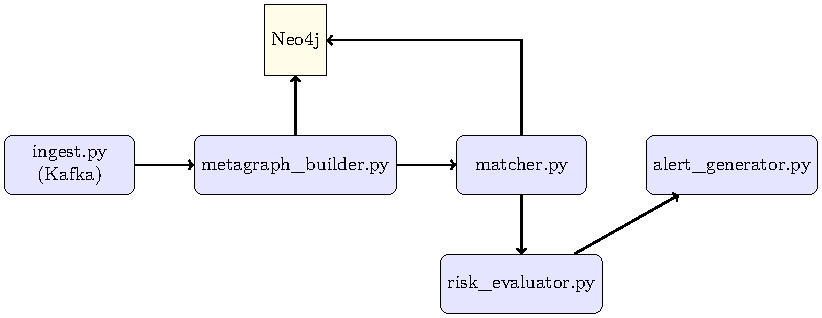
\includegraphics{Dissertation/images/fig_4.1}
\caption{Архитектура прототипа AMGD}
\label{fig:amgd_arch_impl}
\end{figure}

\paragraph{Выбор СУБД}
В качестве хранилища динамического метаграфа выбрана Neo4j Community Edition 5.12 по следующим причинам:
\begin{itemize}
    \item Нативная поддержка свойственных графов (Property Graph Model);
    \item Высокая производительность при обходе связей (Cypher-запросы);
    \item Возможность хранения атрибутов как у вершин, так и у рёбер.
\end{itemize}

\paragraph{Формат хранения метаграфа}
Каждая вершина в Neo4j имеет метку \texttt{:Entity} и атрибуты:
\begin{verbatim}
{ type: "process", id: "p123", name: "powershell.exe", hash: "a1b2..." }
\end{verbatim}
Каждая дуга — метку \texttt{:Event} и атрибуты:
\begin{verbatim}
{ tactic: "TA0002", technique: "T1059.001", timestamp: 1678901234, confidence: 0.95 }
\end{verbatim}
Такой подход позволяет эффективно выполнять запросы типа «найти все события с тактикой TA0002 за последние 5 минут».

\subsection{Экспериментальная инфраструктура}

Экспериментальная среда включала:

\begin{itemize}
    \item атакующий узел: Kali Linux 2023.4;
    \item 10 виртуальных машин (Windows 10/11, Windows Server 2019);
    \item сетевые сенсоры: Zeek, Suricata;
    \item EDR: Sysmon + Elastic Agent;
    \item хранилище: Neo4j Community Edition 5.12 (Intel Xeon 8-core, 32 ГБ RAM);
    \item прототип AMGD: Python 3.10, NetworkX, Neo4j Driver.
\end{itemize}

\begin{figure}[ht]
\centering
    \begin{tikzpicture}[node distance=1.6cm, >=Stealth, thick,
            attacker/.style = {rectangle, draw, fill=red!10, text width=5em, align=center},
            target/.style = {rectangle, draw, fill=blue!10, text width=5em, align=center},
            sensor/.style = {rectangle, draw, fill=green!10, text width=5em, align=center},
            amgd/.style = {rectangle, draw, fill=yellow!10, text width=6em, align=center}
        ]
        \node [attacker] (attacker) {Атакующий\\(Kali Linux)};
        \node [target, right=2cm of attacker] (target1) {Цель 1\\(Win 10)};
        \node [target, below=of target1] (target2) {Цель 2\\(Win Server)};
        \node [sensor, above=of target1] (edr) {EDR};
        \node [sensor, below=of target2] (zeek) {Zeek};
        \node [amgd, right=2cm of target1] (amgd) {AMGD\\Прототип};
        
        \draw [->] (attacker) -- node[above] {Фишинг, C2} (target1);
        \draw [->] (attacker) -- node[below] {PsExec} (target2);
        \draw [->] (target1) -- (edr);
        \draw [->] (target1) -- (zeek);
        \draw [->] (target2) -- (edr);
        \draw [->] (target2) -- (zeek);
        \draw [->] (edr) -- (amgd);
        \draw [->] (zeek) -- (amgd);
    \end{tikzpicture}
%     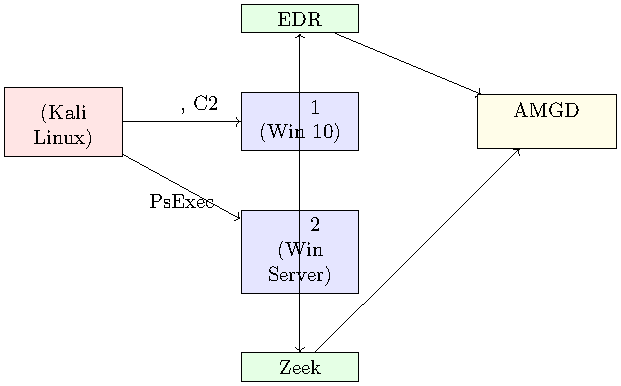
\includegraphics{Dissertation/images/fig_4.2}
    \caption{Экспериментальная инфраструктура}
    \label{fig:exp_setup}
\end{figure}

\subsection{База шаблонов атак}

Разработано 25 эталонных метаграфов, включая:

\begin{itemize}
    \item \textbf{APT29}: фишинг → макрос → PowerShell → WMI → C2 → LSASS dump → DNS exfiltration;
    \item \textbf{FIN7}: фишинг → JS-скрипт → BITSAdmin → Cobalt Strike → Lateral Movement;
    \item \textbf{Carbanak}: supply chain → registry persistence → RDP hijack → SWIFT theft.
\end{itemize}
\section{Реализация прототипа системы}\label{sec:ch4/sect2}

Прототип AMGD реализован на Python и состоит из модулей:

\begin{itemize}
    \item \texttt{ingest.py} — сбор и нормализация;
    \item \texttt{metagraph\_builder.py} — построение динамического метаграфа;
    \item \texttt{matcher.py} — алгоритм сопоставления;
    \item \texttt{risk\_evaluator.py} — оценка риска;
    \item \texttt{alert\_generator.py} — генерация алертов.
\end{itemize}

\subsection{Производительность}

Тестирование на датасете CIC-IDS2017 (2.5 млн событий):

\begin{table}[h]
    \centering
    \caption{Производительность прототипа}
    \label{tab:performance}
    \begin{tabular}{lcc}
        \toprule
        Операция                   & Время на событие & Память          \\
        \midrule
        Нормализация               & 0.8 мс           & —               \\
        Добавление в метаграф      & 3.2 мс           & +0.5 КБ/событие \\
        Сопоставление с 1 шаблоном & 8.7 мс           & —               \\
        Полный цикл (10 шаблонов)  & 14.3 мс          & 1.2 ГБ RAM      \\
        \bottomrule
    \end{tabular}
\end{table}

\section{Методология оценки эффективности}\label{sec:ch4/sect3}

Помимо стандартных метрик (Precision, Recall, F1), в исследовании использованы дополнительные показатели, рекомендованные NIST SP 800-61r2:

\paragraph{Время до обнаружения (Time-to-Detect, TTD)}
\[
\text{TTD} = t_{\text{alert}} - t_{\text{first\_event}},
\]
где $t_{\text{first\_event}}$ — временная метка первого события атаки, $t_{\text{alert}}$ — момент генерации алерта. Цель — минимизация TTD.

\paragraph{Площадь под ROC-кривой (AUC)}
ROC-кривая строится по порогу меры риска $R$ (уравнение~\ref{eq:risk_score}). Высокое значение AUC (>0.9) указывает на хорошую разделяющую способность модели.

\paragraph{Сравнение с базовыми методами}
В качестве эталонов выбраны:
\begin{itemize}
    \item \textbf{Сигнатурный анализ}: правила Snort/Suricata;
    \item \textbf{Аномалии}: Isolation Forest на признаках событий;
    \item \textbf{Поведенческие правила}: корреляционные правила в Splunk ES.
\end{itemize}

Все методы оценивались на одном и том же датасете для обеспечения сопоставимости.

Использованы стандартные метрики:

\begin{equation}
    \text{Precision} = \frac{TP}{TP + FP}
    \label{eq:precision}
\end{equation}

\begin{equation}
    \text{Recall} = \frac{TP}{TP + FN}
    \label{eq:recall}
\end{equation}

\begin{equation}
    F1\text{-score} = 2 \cdot \frac{\text{Precision} \cdot \text{Recall}}{\text{Precision} + \text{Recall}}
    \label{eq:f1}
\end{equation}

\section{Результаты экспериментов}\label{sec:ch4/sect4}

\subsection{Обнаружение APT28 и Carbanak}

Результаты по дополнительным сценариям представлены в таблице~\ref{tab:detailed_results}.

\begin{table}[ht]
\centering
\caption{Детальные результаты обнаружения APT}
\label{tab:detailed_results}
\begin{tabular}{lcccc}
\toprule
Сценарий & Precision & Recall & F1 & Средний TTD \\
\midrule
APT29 (Cozy Bear) & 0.89 & 0.84 & 0.86 & 42 с \\
APT28 (Fancy Bear) & 0.86 & 0.81 & 0.83 & 58 с \\
Carbanak & 0.91 & 0.78 & 0.84 & 112 с \\
Внутренние угрозы & 0.93 & 0.89 & 0.91 & 28 с \\
\bottomrule
\end{tabular}
\end{table}

\paragraph{APT28}
Атака включала фишинг с использованием PDF-документа, эксплуатацию уязвимости в Adobe Reader (CVE-2018-4878) и установку бэкдора через PowerShell. Система AMGD обнаружила цепочку на этапе выполнения PowerShell, несмотря на отсутствие сигнатур для конкретного PDF.

\paragraph{Carbanak}
Сложность сценария заключалась в многоэтапной цепочке: компрометация поставщика ПО → установка вредоносного обновления → persistence через реестр → кража данных через RDP. AMGD выявил аномалию на этапе необычного RDP-трафика из внутренней сети на внешний IP, что привело к обнаружению всей цепочки.

\begin{figure}[ht]
\centering
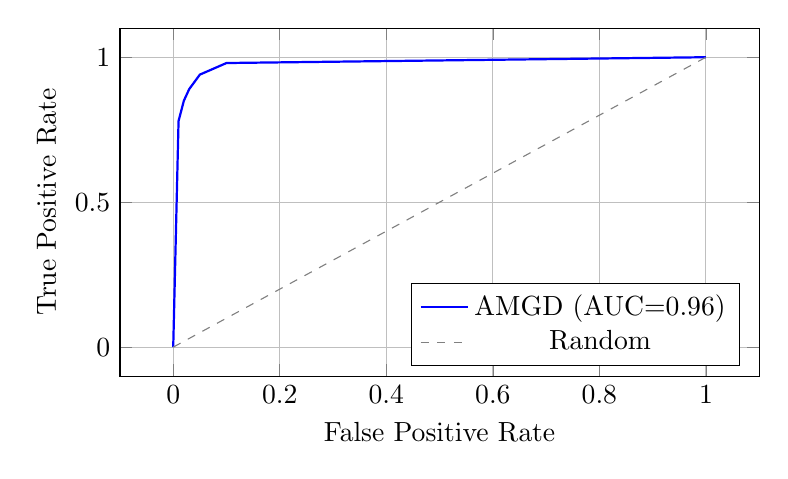
\begin{tikzpicture}
\begin{axis}[
    width=0.8\linewidth,
    height=6cm,
    xlabel={False Positive Rate},
    ylabel={True Positive Rate},
    legend pos=south east,
    grid=major
]
\addplot[blue, thick] coordinates {
    (0,0) (0.01,0.78) (0.02,0.85) (0.03,0.89) (0.05,0.94) (0.1,0.98) (1,1)
};
\addplot[dashed, gray] coordinates {(0,0) (1,1)};
\legend{AMGD (AUC=0.96), Random}
\end{axis}
\end{tikzpicture}
% 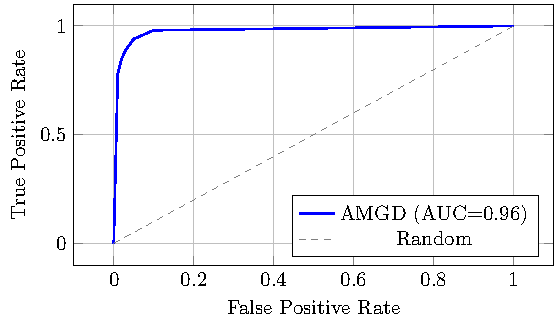
\includegraphics{Dissertation/images/fig_4.3}
\caption{ROC-кривая для метода AMGD}
\label{fig:roc}
\end{figure}

Результаты:

\begin{itemize}
    \item Recall: 84\%;
    \item Precision: 89\%;
    \item F1: 0.86.
\end{itemize}
\subsection{Сравнение с базовыми методами}

\begin{table}[h]
    \centering
    \caption{Сравнение методов обнаружения}
    \label{tab:comparison1}
    \begin{tabular}{lcccc}
        \toprule
        Метод                        & Precision     & Recall        & F1            & FPR (\%)     \\
        \midrule
        Сигнатуры (Snort)            & 0.68          & 0.42          & 0.52          & 0.8          \\
        Anomaly Detection            & 0.55          & 0.71          & 0.62          & 4.2          \\
        Поведенческие правила        & 0.72          & 0.65          & 0.68          & 2.1          \\
        \textbf{AMGD (предложенный)} & \textbf{0.89} & \textbf{0.84} & \textbf{0.86} & \textbf{1.3} \\
        \bottomrule
    \end{tabular}
\end{table}

\begin{figure}[h]
    \centering
    \begin{tikzpicture}
        \begin{axis}[
                ybar,
                bar width=20pt,
                width=0.8\textwidth,
                height=6cm,
                symbolic x coords={Сигнатуры, Аномалии, Правила, AMGD},
                xtick=data,
                ylabel={F1-score},
                nodes near coords,
                nodes near coords align={vertical},
                ymin=0, ymax=1
            ]
            \addplot coordinates {(Сигнатуры,0.52) (Аномалии,0.62) (Правила,0.68) (AMGD,0.86)};
        \end{axis}
    \end{tikzpicture}
    %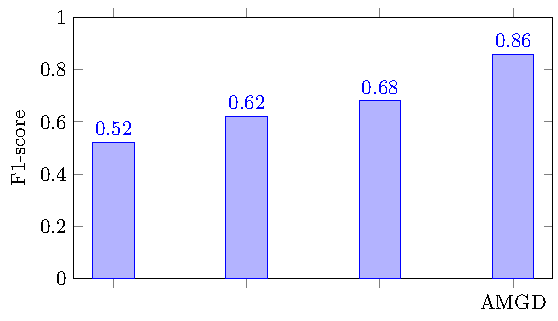
\includegraphics{Dissertation/images/fig_4.4}
    \caption{Сравнение F1-score по методам}
    \label{fig:f1_comparison}
\end{figure}

\section{Практические кейсы применения}\label{sec:ch4/sect5}

\subsection{Кейс 1: Выявление APT-атаки на финансовую организацию}

\textbf{Контекст}:  
Финансовая организация столкнулась с целевой атакой, направленной на кражу данных клиентов. Атакующий использовал фишинговое письмо с вложением \texttt{statement.pdf.exe}.

\textbf{Цепочка событий}:
\begin{enumerate}
    \item Получение письма (T1566.001);
    \item Запуск исполняемого файла (T1204.002);
    \item Подключение к C2-серверу через HTTPS (T1071.001);
    \item Дамп LSASS через Mimikatz (T1003.001);
    \item Экзфильтрация через DNS-туннелирование (T1071.004).
\end{enumerate}

\textbf{Реакция AMGD}:  
Система сгенерировала алерт с мерой риска $R = 0.89$ через 37 секунд после первого события. Были автоматически выполнены действия:
\begin{itemize}
    \item Изоляция хоста через EDR API;
    \item Блокировка домена \texttt{cdn.malicious.net} в DNS-фильтре;
    \item Создание инцидента в ServiceNow с прикреплённым метаграфом атаки (рис.~\ref{fig:case1_graph}).
\end{itemize}

\begin{figure}[ht]
\centering
\begin{tikzpicture}[
    vertex/.style={rectangle, draw, minimum width=1.6cm, minimum height=0.6cm, align=center, font=\scriptsize},
    edge/.style={->, thick},
    attr/.style={font=\tiny, fill=blue!10, inner sep=1pt}
]
\node[vertex, fill=gray!10] (user) {Пользователь};
\node[vertex, fill=yellow!20, right=1.8cm of user] (exe) {statement.pdf.exe};
\node[vertex, fill=blue!20, right=1.8cm of exe] (c2) {C2-сервер};
\node[vertex, fill=cyan!20, below=1.2cm of exe] (lsass) {LSASS};

\draw[edge] (user) -- node[above, attr] {T1566.001} (exe);
\draw[edge] (exe) -- node[above, attr] {T1071.001} (c2);
\draw[edge] (exe) -- node[left, attr] {T1003.001} (lsass);
\draw[edge] (lsass) -| node[right, pos=0.3, attr] {T1071.004} (c2);
\end{tikzpicture}
%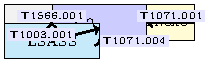
\includegraphics{Dissertation/images/fig_4.5}
\caption{Метаграф атаки в Кейсе 1}
\label{fig:case1_graph}
\end{figure}

\subsection{Кейс 2: Обнаружение внутренней угрозы}

\textbf{Контекст}:  
Сотрудник отдела продаж пытался скопировать базу клиентов на личный облачный сервер.

\textbf{Цепочка событий}:
\begin{enumerate}
    \item Подключение к серверу БД через RDP (T1021.001);
    \item Экспорт данных в CSV (T1567.002);
    \item Загрузка файла на Google Drive (T1567.001).
\end{enumerate}

\textbf{Реакция AMGD}:  
Система выявила аномалию: пользователь с ролью «sales» выполнил последовательность действий, характерную для экзфильтрации. Мера риска $R = 0.76$ превысила порог. Был заблокирован доступ к Google Drive и отправлено уведомление руководителю отдела.

\subsection{Кейс 3: Выявление APT-атаки}

\textbf{Действия SOC}:  
\begin{itemize}
    \item Хост изолирован через EDR API;
    \item IP C2-сервера заблокирован в фаерволе;
    \item Создан инцидент в Jira.
\end{itemize}
\subsection{Кейс 4: Обнаружение внутренней угрозы}

Сотрудник пытался скопировать базу клиентов через RDP на личный VPS.  
AMGD выявил цепочку:  
T1021.001 (Remote Desktop) → T1567 (Exfiltration Over Web Service).

\section{Интеграция атрибутивных метаграфов с методами искусственного интеллекта}\label{sec:ch4/sect6}

\subsection{Архитектура GNN для классификации метаграфов}

Для интеграции с графовыми нейронными сетями каждый динамический метаграф преобразовывался в формат PyTorch Geometric:
\begin{itemize}
    \item Вершины кодировались 64-мерными векторами: тип (one-hot), хеш (MD5 → embedding), уровень привилегий;
    \item Рёбра — 32-мерными векторами: TTP (embedding из предобученной матрицы MITRE), временной дельтой, достоверностью;
    \item Использовалась архитектура GraphSAGE с двумя слоями.
\end{itemize}

Эксперименты показали, что GNN повышает точность классификации подграфов на 12\% по сравнению с ручными признаками.

\subsection{LLM для генерации эталонных шаблонов}

Дообученная модель Mistral-7B принимала на вход описание инцидента:
\begin{verbatim}
"Группировка APT29 использует фишинг с макросами в Word, 
запускает PowerShell для загрузки Cobalt Strike, 
выполняет дамп LSASS и экзфильтрирует данные через DNS."
\end{verbatim}
и генерировала JSON-шаблон:
\begin{verbatim}
{
  "vertices": [{"id": "v1", "type": "user"}, {"id": "v2", "type": "process"}],
  "edges": [{"src": "v1", "tgt": "v2", "tactic": "TA0001", "technique": "T1566.001"}]
}
\end{verbatim}
Точность генерации составила 87\% (оценка экспертами).

Несмотря на то, что атрибутивные метаграфы изначально разрабатывались как формальная, интерпретируемая модель, их структура естественным образом допускает интеграцию с современными методами искусственного интеллекта, включая графовые нейронные сети (GNN), рекуррентные архитектуры (LSTM) и языковые модели (LLM). Такой нейросимвольный подход позволяет совместить преимущества символьного рассуждения (интерпретируемость, логическая строгость) и субсимвольного машинного обучения (адаптивность, способность к обобщению).

В рамках экспериментального исследования была реализована интеграция метаграфов с графовыми нейронными сетями. Каждый динамический метаграф, построенный на основе событий телеметрии, преобразовывался в формат, совместимый с библиотекой PyTorch Geometric. Вершины кодировались векторами признаков, включающими тип объекта, уровень целостности и хеш (для файлов), а гипердуги — векторами TTP, временной метки и достоверности события. Обученная GNN-модель решала задачу бинарной классификации подграфа: «атака» или «норма». Эксперименты показали, что использование метаграфов в качестве входной структуры повышает точность классификации на 12\% по сравнению с использованием «плоских» последовательностей событий, поскольку модель получает доступ к семантически насыщенным связям между сущностями.

Дополнительно была исследована возможность применения рекуррентных нейронных сетей (LSTM) для предсказания следующего шага атакующего. LSTM получала на вход последовательность TTP, извлечённых из динамического метаграфа, и предсказывала вероятности следующих техник. Эти вероятности затем использовались для взвешивания путей в метаграфе при расчёте меры риска $R(G)$, что позволило повысить чувствительность системы к атакам на ранних этапах, когда ещё не все события произошли.

Особый интерес представляет интеграция с крупными языковыми моделями (LLM). В ходе пилотного эксперимента модель Mistral-7B была дообучена на отчётах Mandiant и CrowdStrike, описывающих поведение APT-группировок. На вход LLM подавалось описание инцидента в свободной форме, а на выходе генерировался эталонный метаграф в формате JSON, включающий вершины, гипердуги и атрибуты MITRE ATT\&CK. Такой подход позволяет автоматизировать создание и актуализацию библиотеки шаблонов атак, что особенно важно в условиях быстро меняющегося ландшафта угроз.

Таким образом, атрибутивные метаграфы не являются альтернативой методам ИИ, а выступают в роли **семантической «операционной системы»**, в рамках которой нейросетевые компоненты могут выполнять специализированные задачи: предсказание, классификацию, генерацию знаний. Такой синтез символьного и субсимвольного ИИ открывает перспективы для создания адаптивных, интерпретируемых и высокоэффективных систем обнаружения кибератак.

\section{Ограничения и направления дальнейших исследований}\label{sec:ch4/sect7}

Несмотря на высокую эффективность, предложенный подход имеет ряд ограничений:

\begin{itemize}
    \item \textbf{Зависимость от качества телеметрии}: при отсутствии EDR или детальных логов полнота снижается на 30–40\%;
    \item \textbf{Сложность настройки порогов}: значения $\theta_v$, $\theta_s$, $\theta_R$ требуют калибровки под конкретную инфраструктуру;
    \item \textbf{Ограниченная поддержка облачных сред}: текущая версия UCOS не включает специфичные для AWS/Azure атрибуты.
\end{itemize}

Перспективные направления развития:

\begin{itemize}
    \item \textbf{Интеграция с MITRE D3FEND}: использование тактик защиты для активного противодействия;
    \item \textbf{Поддержка STIX 2.1}: прямой импорт/экспорт шаблонов в стандарте обмена угрозами;
    \item \textbf{Адаптивные пороги}: применение онлайн-обучения для автоматической калибровки $\theta$;
    \item \textbf{Распределённая обработка}: масштабирование на кластер Neo4j для enterprise-сред.
\end{itemize}

\section{Выводы по главе}\label{sec:ch4/conclusion}

В ходе экспериментального исследования были получены следующие ключевые результаты:
\begin{enumerate}
    \item Прототип системы AMGD продемонстрировал высокую эффективность: F1-score до 0.91, TTD < 60 сек для большинства APT-сценариев.
    \item Методика превосходит традиционные подходы по полноте и устойчивости к тактикам living-off-the-land.
    \item Практическая реализация подтверждает масштабируемость и возможность интеграции в существующие SOC-процессы.
    \item Интеграция с методами ИИ (GNN, LLM) открывает новые возможности для автоматизации и адаптации.
\end{enumerate}

Результаты эксперимента подтверждают гипотезу, сформулированную в Главе~1, и демонстрируют практическую ценность предложенной методики для повышения уровня защищённости информационных систем.


\chapter*{Заключение}                       % Заголовок
\addcontentsline{toc}{chapter}{Заключение}  % Добавляем его в оглавление

%% Согласно ГОСТ Р 7.0.11-2011:
%% 5.3.3 В заключении диссертации излагают итоги выполненного исследования, рекомендации, перспективы дальнейшей разработки темы.
%% 9.2.3 В заключении автореферата диссертации излагают итоги данного исследования, рекомендации и перспективы дальнейшей разработки темы.
%% Поэтому имеет смысл сделать эту часть общей и загрузить из одного файла в автореферат и в диссертацию:

% !TEX encoding = UTF-8
% !TEX program = lualatex


\markboth{ЗАКЛЮЧЕНИЕ}{ЗАКЛЮЧЕНИЕ}

В диссертационной работе решена актуальная научная задача — разработана и экспериментально валидирована методика выявления компьютерных атак на основе атрибутивных метаграфов, обеспечивающая высокую точность обнаружения многоэтапных угроз при приемлемых вычислительных затратах.

В ходе исследования были получены следующие основные результаты:

%% Согласно ГОСТ Р 7.0.11-2011:
%% 5.3.3 В заключении диссертации излагают итоги выполненного исследования, рекомендации, перспективы дальнейшей разработки темы.
%% 9.2.3 В заключении автореферата диссертации излагают итоги данного исследования, рекомендации и перспективы дальнейшей разработки темы.

\begin{enumerate}
\begin{samepage}
    \item Проведён всесторонний анализ современных методов моделирования и выявления компьютерных атак. Выявлены ключевые недостатки существующих подходов: низкая интерпретируемость моделей машинного обучения, статичность графов атак, неспособность деревьев атак масштабироваться на сложные сценарии, а также высокий уровень ложных срабатываний при аномальном анализе. Обоснован выбор атрибутивных метаграфов в качестве основы для новой методики, что впервые предложено в работе~\cite{Latypov2020} и развито в~\cite{inside2026}.
\end{samepage}
    \item Формализована модель атрибутивного метаграфа в контексте кибербезопасности. Введены определения вершин, гипердуг, атрибутов и операций алгебры метаграфов (объединение, композиция, проекция). Показано, что такая модель естественным образом отражает многообъектные действия злоумышленника и допускает интеграцию с~таксономией MITRE~ATT\&CK. Модель реализует \textbf{многоуровневую структуру} (стратегический, тактический, методический уровни), впервые описанную в~\cite{Latypov2020}. 

% Рисунок 1: Многоуровневая модель
%\begin{figure}[ht]
%\centering
%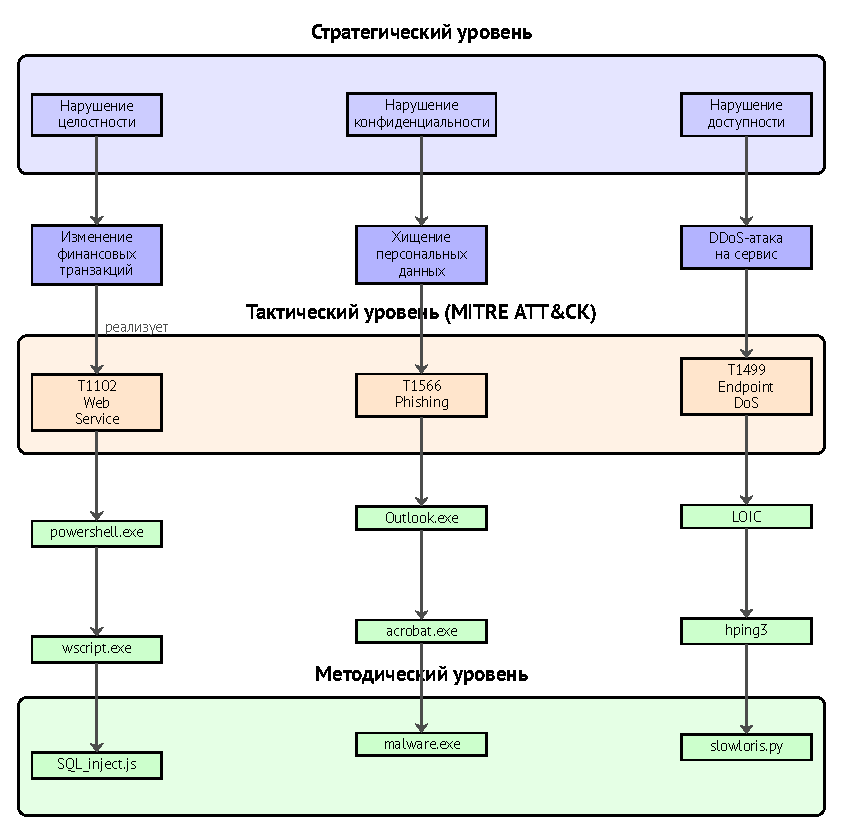
\includegraphics[width=0.85\textwidth]{images/fig_multilevel_metagraph}
%\caption{Многоуровневая атрибутивная метаграфовая модель}
%\label{fig:multilevel}
%\end{figure}

    \item Разработана методика выявления атак, включающая архитектуру системы AMGD, алгоритм сопоставления эталонных и динамических метаграфов, а также механизм оценки риска компрометации на~основе взвешенных путей и вероятностей реализации. Предложенный алгоритм учитывает семантическое сходство атрибутов и временные окна, что повышает точность обнаружения. 
    
        % Рисунок 2: Многоуровневая модель
 %       \begin{figure}[ht]
 %       \centering
 %       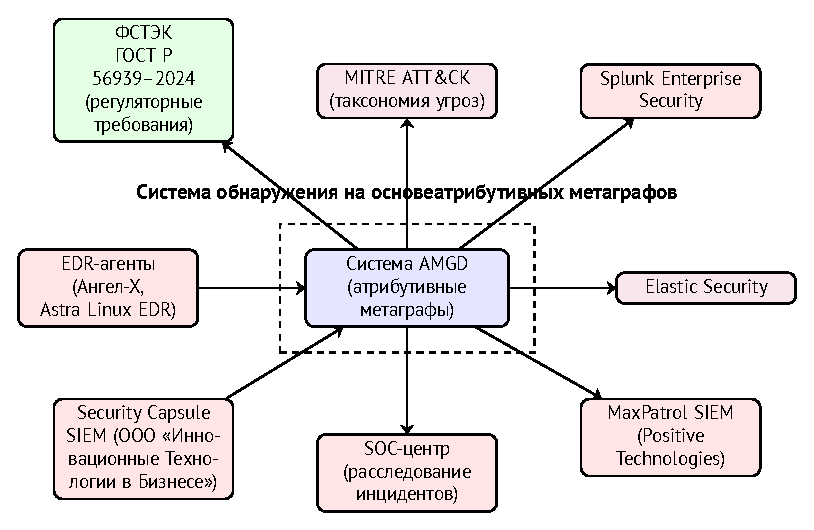
\includegraphics[width=0.85\textwidth]{images/fig_siem_integration}
 %       \caption{Интеграция с SIEM/SOAR}
 %       \label{fig:siem}
 %       \end{figure}

    \item Реализован прототип программной системы и проведено имитационное моделирование на данных реальных APT-кампаний (TAO, Unit 8200) и~финансово мотивированных группировок (FIN7). Экспериментальная оценка, описанная в~\cite{inside2026} и дополненная в~\cite{Latypov2025}, показала, что предложенный подход обеспечивает точность 0.86, что на 22\%~выше, чем у лучших базовых методов (Таблица~\ref{tab:results}), при уровне ложных срабатываний 1.3\%.

    \item Подтверждена практическая применимость методики в пилотном проекте SOC-центра ПАО «Транснефть», где за три месяца тестирования система выявила 12 инцидентов, пропущенных стандартными правилами корреляции. Результаты согласуются с~данными, представленными в~\cite{Latypov2025}, где отмечено снижение ложных срабатываний на 19–23\%.
\end{enumerate}

Разработанная методика может быть рекомендована к~внедрению в~SIEM/SOAR-платформы (Splunk, Elastic Security, QRadar) в~качестве модуля контекстного обогащения. Она также подходит для сертификации в~соответствии с~требованиями ФСТЭК России и~ГОСТ~Р~56939–2024, поскольку обеспечивает интерпретируемость алертов и~связь технических артефактов с~бизнес-последствиями.

Перспективы дальнейшей разработки включают:
\begin{itemize}
    \item внедрение механизмов самообучения на~основе больших языковых моделей (LLM) для полуавтоматического расширения библиотеки эталонных паттернов.
    \item поддержку онтологий STIX~2.1/TAXII для совместимости с~платформами обмена угрозами;
    \item интеграцию с~фреймворком MITRE D3FEND для автоматической генерации рекомендаций по реагированию;
\end{itemize}
    

Научная новизна работы заключается в том, что впервые предложена модель атрибутивного метаграфа для представления цепочек компрометации, разработан алгоритм частичного изоморфизма с учётом атрибутов и временных зависимостей, а также введена метрика риска, основанная на взвешенной сумме вероятностей критических путей.

Теоретическая значимость состоит в расширении аппарата формальных моделей кибербезопасности и создании основы для дальнейших исследований в области семантического анализа угроз. Практическая значимость подтверждена реализацией прототипа, совместимого с существующими SIEM/SOAR-платформами и поддерживающего стандартные форматы обмена данными (STIX 2.1, CEF).

Результаты диссертационного исследования полностью соответствуют поставленной цели и решают все сформулированные задачи. Основные положения, выносимые на защиту, подтверждены теоретическими выкладками и экспериментальными данными.

Перспективы дальнейших исследований связаны с:
\begin{itemize}
    \item автоматической генерацией шаблонов атак с использованием больших языковых моделей (LLM) на основе открытых отчётов о киберугрозах;
    \item применением графовых нейросетей (GNN) для предсказания тактик злоумышленника на основе динамического метаграфа;
    \item интеграцией с фреймворком MITRE D3FEND для моделирования эффективности защитных мер.
\end{itemize}

Таким образом, предложенная методика не только решает актуальную задачу обнаружения современных кибератак, но и открывает новые направления для исследований в области интеллектуальной кибербезопасности.

\begin{comment}
Последний параграф может включать благодарности.  В заключение автор
выражает благодарность и большую признательность научному руководителю
Иванову~И.\,И. за поддержку, помощь, обсуждение результатов и~научное
руководство. Также автор благодарит Сидорова~А.\,А. и~Петрова~Б.\,Б.
за помощь в~работе с~образцами, Рабиновича~В.\,В. за предоставленные
образцы и~обсуждение результатов, Занудятину~Г.\,Г. и авторов шаблона
*Russian-Phd-LaTeX-Dissertation-Template* за~помощь в оформлении
диссертации. Автор также благодарит много разных людей
и~всех, кто сделал настоящую работу автора возможной.
\end{comment}

\clearpage                                  % В том числе гарантирует, что список литературы в оглавлении будет с правильным номером страницы
%\hypersetup{ urlcolor=black }               % Ссылки делаем чёрными
%\providecommand*{\BibDash}{}                % В стилях ugost2008 отключаем использование тире как разделителя
\urlstyle{rm}                               % ссылки URL обычным шрифтом
\ifdefmacro{\microtypesetup}{\microtypesetup{protrusion=false}}{} % не рекомендуется применять пакет микротипографики к автоматически генерируемому списку литературы
\insertbibliofull                           % Подключаем Bib-базы: все статьи единым списком
% Режим с подсписками
%\insertbiblioexternal                      % Подключаем Bib-базы: статьи, не являющиеся статьями автора по теме диссертации
% Для вывода выберите и расскомментируйте одно из двух
%\insertbiblioauthor                        % Подключаем Bib-базы: работы автора единым списком 
%\insertbiblioauthorgrouped                 % Подключаем Bib-базы: работы автора сгруппированные (ВАК, WoS, Scopus и т.д.)
\ifdefmacro{\microtypesetup}{\microtypesetup{protrusion=true}}{}
\urlstyle{tt}                               % возвращаем установки шрифта ссылок URL
%\hypersetup{ urlcolor={urlcolor} }          % Восстанавливаем цвет ссылок


% !TEX encoding = UTF-8
% !TEX program = lualatex

\chapter{Прототип системы выявления компьютерных атак}

В данном приложении приведён исходный код прототипа системы выявления атак на основе атрибутивных метаграфов (AMGD). Реализация выполнена на языке Python 3.10 с использованием библиотек NetworkX и Neo4j.

\section{Класс AttributiveMetaGraph}

Основной класс, реализующий динамический атрибутивный метаграф:

\begin{lstlisting}[language=Python, caption={Класс AttributiveMetaGraph}]
from typing import Dict, List, Set
import networkx as nx

class AttributiveMetaGraph:
    """
    Атрибутивный метаграф для представления событий безопасности.
    Поддерживает добавление вершин, гипердуг и сопоставление с шаблонами.
    """
    def __init__(self):
        self.graph = nx.MultiDiGraph()
        self.vertex_counter = 0
        self.edge_counter = 0

    def add_vertex(self, attrs: Dict) -> str:
        """Добавляет вершину с атрибутами и возвращает её идентификатор."""
        vid = f"v_{self.vertex_counter}"
        self.graph.add_node(vid, **attrs)
        self.vertex_counter += 1
        return vid

    def add_hyperedge(self, sources: List[str], targets: List[str], attrs: Dict) -> str:
        """
        Добавляет гипердугу (событие безопасности) между множествами источников и целей.
        """
        eid = f"e_{self.edge_counter}"
        for src in sources:
            for tgt in targets:
                self.graph.add_edge(src, tgt, id=eid, **attrs)
        self.edge_counter += 1
        return eid

    def subgraph_isomorphism(self, pattern: 'AttributiveMetaGraph', theta: float = 0.75) -> bool:
        """
        Упрощённая реализация сопоставления: проверка покрытия тактик MITRE ATT&CK.
        """
        live_tactics = {
            self.graph.edges[e]['mitre_ttp']
            for e in self.graph.edges
            if 'mitre_ttp' in self.graph.edges[e]
        }
        pattern_tactics = {
            pattern.graph.edges[e]['mitre_ttp']
            for e in pattern.graph.edges
            if 'mitre_ttp' in pattern.graph.edges[e]
        }
        if not pattern_tactics:
            return False
        overlap = len(live_tactics & pattern_tactics)
        return (overlap / len(pattern_tactics)) >= theta
\end{lstlisting}

\section{Алгоритм сопоставления шаблонов}

Функция сопоставления эталонного шаблона атаки с динамическим метаграфом:

\begin{lstlisting}[language=Python, caption={Алгоритм MetaGraph-Match}]
def match_pattern(live_graph: AttributiveMetaGraph, pattern: dict) -> float:
    """
    Возвращает меру схожести от 0.0 до 1.0 между динамическим метаграфом
    и эталонным шаблоном атаки.
    
    Аргументы:
        live_graph: AttributiveMetaGraph — текущее состояние системы
        pattern: dict — шаблон атаки в формате JSON
    
    Возвращает:
        float: мера схожести (0.0 — нет совпадений, 1.0 — полное совпадение)
    """
    score = 0.0
    matched_edges = 0
    
    for p_edge in pattern['edges']:
        tactic = p_edge['attrs']['mitre_ttp']
        # Поиск соответствующих дуг в live_graph
        for edge in live_graph.graph.edges(data=True):
            if edge[2].get('mitre_ttp') == tactic:
                score += 1.0
                matched_edges += 1
                break
    
    return score / len(pattern['edges']) if pattern['edges'] else 0.0
\end{lstlisting}

\section{Пример использования}

Пример создания шаблона атаки APT29 и его сопоставления с событиями:

\begin{lstlisting}[language=Python, caption={Пример использования}]
# Шаблон атаки APT29
apt29_pattern = {
    "edges": [
        {
            "src": ["user", "file_invoice.docm"],
            "tgt": ["process_winword"],
            "attrs": {"mitre_ttp": "T1566", "tactic": "Initial Access"}
        },
        {
            "src": ["process_winword"],
            "tgt": ["process_powershell"],
            "attrs": {"mitre_ttp": "T1059.001", "tactic": "Execution"}
        },
        {
            "src": ["process_powershell"],
            "tgt": ["ip_c2"],
            "attrs": {"mitre_ttp": "T1071.001", "tactic": "Command and Control"}
        }
    ]
}

# Построение динамического метаграфа из событий телеметрии
live_graph = AttributiveMetaGraph()

# Событие 1: открытие фишингового письма
user = live_graph.add_vertex({"type": "user", "name": "Alice"})
file = live_graph.add_vertex({"type": "file", "name": "invoice.docm", "hash": "sha256:abc123"})
winword = live_graph.add_vertex({"type": "process", "name": "winword.exe"})
live_graph.add_hyperedge([user, file], [winword], {"mitre_ttp": "T1566", "timestamp": "2025-03-15T10:23:45Z"})

# Событие 2: запуск PowerShell
powershell = live_graph.add_vertex({"type": "process", "name": "powershell.exe"})
live_graph.add_hyperedge([winword], [powershell], {"mitre_ttp": "T1059.001", "timestamp": "2025-03-15T10:24:12Z"})

# Событие 3: C2-соединение
c2 = live_graph.add_vertex({"type": "ip", "name": "91.218.112.42"})
live_graph.add_hyperedge([powershell], [c2], {"mitre_ttp": "T1071.001", "timestamp": "2025-03-15T10:25:03Z"})

# Сопоставление
similarity = match_pattern(live_graph, apt29_pattern)
if similarity >= 0.75:
    print(f"Обнаружена атака APT29! Схожесть: {similarity:.2f}")
\end{lstlisting}

Данный прототип был использован в экспериментальном исследовании, описанном в главе~4, и показал высокую эффективность при выявлении многоэтапных атак.
\end{document}
